\documentclass{ldbc}

\usepackage{multirow}
\usepackage{float}
\usepackage{amsfonts}
\usepackage{bbding}
\usepackage{rotating}
\usepackage{pifont}
\usepackage{rotating}
\usepackage{subfigure}
\usepackage{amsmath}
\usepackage{longtable}
\usepackage{tabularx}
\usepackage{hyperref}
\usepackage{xspace}
\usepackage[table]{xcolor}
\usepackage{listings}
\providecommand{\tightlist}{%
	\setlength{\itemsep}{0pt}\setlength{\parskip}{0pt}}
\usepackage[export]{adjustbox}

\newcommand{\asc}{\uparrow}
\newcommand{\desc}{\downarrow}

\newcommand{\patternscale}{0.43}
\newcommand{\varname}[1]{\texttt{#1}}
\newcommand{\vartype}[1]{\footnotesize \textsf{#1}}
\newcommand{\variable}[2]{
	\renewcommand*{\arraystretch}{1}
	\begin{tabular}{|c|c|}\hline \varname{#1} & \cellcolor{gray!20} \vartype{#2}\\\hline\end{tabular}
	\renewcommand*{\arraystretch}{1.95}
}
\newcommand{\sortentry}[2]{
	\renewcommand*{\arraystretch}{1}
	\begin{tabular}{|c|c|}\hline \varname{#1} & $#2$\\\hline\end{tabular}
	\renewcommand*{\arraystretch}{1.95}
}
\newcommand{\chokepoint}[1]{\hyperref[choke_point_#1]{#1}}

\newcommand{\cmark}{\ding{51}}%
\newcommand{\xmark}{\ding{55}}%
\newcommand{\yes}{\color{green}\ding{51}\color{black}}
\newcommand{\no}{\color{red}\ding{55}\color{black}}

\newcommand{\cref}[1]{Chapter~\ref{#1}}
\newcommand{\sref}[1]{Section~\ref{#1}}
\newcommand{\tref}[1]{Table~\ref{#1}}
\newcommand{\fref}[1]{Figure~\ref{#1}}
\newcommand{\eref}[1]{Equation~\ref{#1}}
\newcommand{\aref}[1]{Appendix~\ref{#1}}

% Alex Averbuch: used internally only, to make missing/erroneous sections stand out
\newcommand{\alert}[1]{\textit{\textbf{{\color{red}#1}}}}

% todo change the following information as appropriate
%\WP{N/A}
\renewcommand{\wpIDText}{N/A}
\WPTitle{Social Network Benchmark Task Force}

%\delID{}
\renewcommand{\delIDText}{}
\delName{LDBC Social Network Benchmark (SNB) - v0.2.4 }

\dueDate{M12}
\submissionDate{M13}

%dissemination level
\dissPU % Public
%\dissRE % Restricted to group
%\dissPP % Restricted to programme
%\dissCO % Consortium-only

%nature
\natR % Report
%\natP % Prototype
%\natD % Demonstrator
%\natO % Other

%\author{[Arnau Prat (UPC)]}
%\authorPartner{Arnau Prat (UPC)}
%\responsibleAuthor{Arnau Prat}
%\responsiblePartner{UPC}
%\responsiblePhone{+34934054032}
%\responsibleEmail{aprat@ac.upc.edu}

% comment the following out if there are no contributors beside the main authors
%\contributor{[Peter Boncz (VUA), Josep Llu\'is Larriba (UPC), Renzo
%Angles (TALCA), Alex Averbuch (NEO), Orri Erling (OGL), Andrey
%Gubichev (TUM), Mirko Spasi\'c (OGL)], Minh-Duc Pham (VUA), Norbert Mart\'inez (SPARSITY)}

\reviewerOne{\alert{???}}
\reviewerTwo{\alert{???}}

\keywords{benchmark, choke points, dataset generator, graph database, query set, RDF, workload, auditing rules, publication rules, scale factors}

% for version numbers, use 2 digits separated by a dot (First digit is
% 0 for ``draft'', 1 for ``project approved'', 2 for ``further revisions''
% such as when the EC rejected version 1
\versionLog{
    \versionLogEntry{19/05/2014}{0.1}{Arnau Prat}{First draft}
}
\lastVersion{0.1}

% uncomment the following for final version
%\final

\documentUrl{\url{https://svn.sti2.at/ldbc/trunk/sib_spec/sib_spec.tex/}}
%\rhead{
\includegraphics[width=0.2\linewidth]{./figures/ldbc-logo.png}}

\abstract{
LDBC's Social Network Benchmark (\ldbcsnb) is an effort intended to test
various functionalities of systems used for graph-like data management. For this,
\ldbcsnb uses the recognizable scenario of operating a social network, characterized by
its graph-shaped data.

\ldbcsnb consists of two workloads that focus on different
functionalities: the Interactive workload (interactive transactional queries)
and the Business Intelligence workload (analytical queries). 

This document contains the definition of both workloads. This includes a detailed
explanation of the data used in the \ldbcsnb benchmark, a detailed description
for all queries, and instructions on how to generate the data and run the
benchmark with the provided software.
}

\execSummary{

The new data economy era, based on complexly structured, distributed and large
datasets, has brought on new demands on data management and analytics.  As a
consequence, new industry actors have appeared, offering technologies specially
built for the management of graph-like data. Also, traditional database
technologies, such as relational databases, are being adapted to the new
demands to remain competitive.

LDBC's Social Network Benchmark (\ldbcsnb) is an industrial and academic
initiative, formed by principal actors in the field of graph-like data
management. Its goal is to define a framework where different graph based
technologies can be fairly tested and compared, that can drive the
identification of systems' bottlenecks and required functionalities, and can
help researchers to open new research frontiers.

The philosophy around which \ldbcsnb is designed is to be easy to
understand, flexible and cheap to adopt. For all these reasons,
\ldbcsnb will propose different workloads representing all the usage scenarios
of graph-like database technologies, hence, targeting systems of different
nature and characteristics.  In order increase its adoption by industry and
research institutions, \ldbcsnb provides all necessary software, which are
designed to be easy to use and deploy at a small cost.

This document contains:
\begin{itemize}
\item A detailed specification of the data used in the whole \ldbcsnb benchmark.
\item A detailed specification of the workloads.
\item A detailed specification of the execution rules of the benchmark.
\item A detailed specification of the auditing rules and the full disclosure
  report's required contents.
\end{itemize}
}


\begin{document}

\maketitle

%\include{glossary}

\chapter*{Special thanks}
Special thanks to all the people that have contributed to the development of
this benchmark:
\begin{itemize}
  \item Renzo Angles (Universidad de Talca)
  \item Alex Averbuch (Neo Technologies)
  \item Peter Boncz (Vrije Universiteit Amsterdam)
  \item Orri Erling (Google)
  \item Andrey Gubichev (Google)
  \item Moritz Kaufmann (Technische Universit\"at M\"unchen)
  \item Josep Llu\'is Larriba Pey (Universitat Polit\`ecnica de Catalunya)
  \item Minh-Duc Pham (Altran)
  \item Marcus Paradies (SAP)
  \item Arnau Prat (Sparsity Technologies)
  \item Mirko Spasi\'c (Openlink Software)
  \item Norbert Mart\'inez (Huawei Technologies)
\end{itemize}

\listoffigures
\listoftables
\chapter*{Definitions}
\chapter*{Definitions}

This section defines fundamental concepts used in the LDBC benchmark terminology. Part of the definitions below are repeated from the LDBC benchmark specification document.

\begin{description}
    \item[\ldbcsnb] The Linked Data Benchmark Council's Social Network Benchmark suite which currently consists of the Interactive workload and a preliminary version of the Business Intelligence workload.
    
    \item[System Under Test (SUT)] This is the totality of the hardware and software that participates in a benchmark run, excluding parts that are exclusively used for driving the workload. If the parts driving the workload are collocated on the same operating system instance as the SUT, then this is also considered a part of the SUT. In client-server configurations where the test driver is not on a machine hosting any DBMS function the SUT is not considered to encompass the hardware or software which exclusively serves to drive the test workload.
    
    \item[\datagen] This module is provided by LDBC SNB and produces the standard benchmark datasets to be loaded into the SUT for the benchmark. The data generation phase is not part of running the benchmark.
 
    \item[Test Driver (Benchmark Driver, Driver)] The test driver refers to the parts of the benchmark run that coordinate query execution and, if prescribed by a given benchmark, data loading.
    
    \item[Workload (Benchmark)] This is the totality of the tasks a particular benchmark performs against an SUT. This includes data loading as well as the query/update workload. This does not include preparatory stages such as generating benchmark data with a data generator or transferring the data to the platform constituting the SUT. 
    The terms workload and benchmark are synonyms in this context. 

    \item[Time Compression Ratio (TCR)]
    This parameter of the Interactive workload compresses (or stretches) durations between operation start times to increase (or decrease) operation rate, thereby allowing systems to reach their maximum throughput for a given workload. The smaller this number is, the higher compression ratio it represents (\eg 2.0 means run benchmark 2x slower, while 0.1 = run benchmark 10x faster). Systems are expected to compete on achieving high $\text{TCR}^{-1}=\frac{1}{\text{TCR}}$.
    
    \item[Query mix] The ratio of read and update queries of a workload, and the frequency at which they are issued.
    
    \item[Scale Factor (SF)] The \ldbcsnb is designed to target systems of different size and scale. The scale factor determines the size of the data used to run the benchmark. The scale factor refers to the measured size of the data in Gigabytes when serialised in CsvSingularProjectedFK.

    \item[Validation Step] The benchmark specifies a scale factor for which ACID test cases are executed and the query results are compared to a reference result set (\ie expected output). This step is required to use the very same set of queries and data structures (this includes both PDS, IADS and EADS -- defined below) that are used in the actual benchmark runs. 
    
    \item[Schema (Database Schema)] A schema is the totality of the non-built-in declarations which are fed into the SUT prior to running a workload. For a relational system, the schema consists of tables, indices, views, materialised views and declarative constraints (\eg foreign key and not null constraints). An ontology for an RDF system counts as a schema if it is loaded on the SUT. An RDF SUT may have no schema at all and still run the workload. However, any declaration or setting (\eg indices) that is not on by default in the SUT, but is used in at least one case of the benchmark run counts as part of the schema.
    The schema does not include stored procedures, triggers, or other imperative (procedural) application specific code that may reside on the SUT and could impact the benchmark results. The schema is required to be the same across all benchmark runs using the same scale factor for a given workload.

    \item[Primary Data Structure (PDS)] 
    This is anything that may influence the result of a database query or may be changed by an update of the database. These may be resident in RAM or durable media or both. Examples of data structures are database base tables and adjacency lists.

    \item[Implicit Auxiliary Data Structure (IADS)] This is a data structure for providing more efficient access to all or parts of the primary data structure. IADS are created by the DBMS automatically and the system may allow them to be turned off. 
    \begin{quote}
        Some systems, such as many RDF stores have multiple covering indices on the primary data structure. The definition in this case is that the primary data structure consists of all the differently ordered full copies of the base table; a table of subject predicate object graph (SPOG) in the RDF case. In this same instance, Auxiliary data structures comprise any data structure which materialise a subset of the SPOG.    
    \end{quote}
    
    \item[Explicit Auxiliary Data Structure (EADS)] These are any application or workload profile specific structures that are declared in addition to the PDSs and IADSs managed by the SUT. These duplicate the data and are created with explicit statements. Secondary indices, materialised views, with or without aggregates, are all examples of this in a relational context. 
    %In an RDF context an EADS is a data structure which holds some of the triples/quads in whole or in part but does not hold some others. 
    The decision about the used EADS is always part of the schema declaration.
    \begin{quote}
        In the case of relational systems, an ADS may be an index from primary key values to a heap table, if the system in question has such concepts. 
        A secondary index of a relational table, in its memory based and durable media based manifestations is an example for EADS. Such a secondary index is not considered an ADS since it must be declared, which makes its creation explicit. An ADS must be implicit and not created by any specific DDL statement or directive. In the case of RDF systems, if the implementation supports user definable index schemes, as long as these are defined once and apply to all triples/quads, such structures are designated as ADS. If an RDF system selectively makes data structures which apply to some quads but not to others, then such structures are designated as EADS.
    \end{quote}

    \item[SUT-Resident Logic] This is any application specific code that is resident on the SUT, whether by static linking, dynamic loading, JIT, interpretation or any other means of embedding application specific logic into a generic DBMS. Examples of this are stored procedures, hosting Java, CLR or other run times in the SUT process (or processes), loading application specific libraries to extend native functions or data structures etc. A special case is that of a database exclusively accessed via an in-process API. In these cases, any code that is not the test driver or a workload implementation expressed against a generally supported API of the DBMS is deemed SUT resident logic in addition to any other code which may fit the above definitions.

    \item[Test Sponsor] The party which initiates an audit of a benchmark implementation over an SUT. This is typically the vendor of a key component of the SUT, \eg DBMS or hardware.

    \item[Full Disclosure Report (FDR)] This is a document which allows reproduction of any audited benchmark result by a third party. It contains complete description of the circumstances of the benchmark run, including version and configuration of SUT, dataset and test driver.
    
\end{description}


\chapter{Introduction}
\chapter{Introduction}
\label{sec:introduction}

%%%%%%%%%%%%%%%%%%%%%%%%%%%%%%%%%%%%%%%%%%%%%%%%%%%%%%%%%%%%%%%%%%%%%%%%%%%%%%
%%%%%%%%%%%%%%%%%%%%%%%%%%%%%%%%%%%%%%%%%%%%%%%%%%%%%%%%%%%%%%%%%%%%%%%%%%%%%%
%%%%%%%%%%%%%%%%%%%%%%%%%%%%%%%%%%%%%%%%%%%%%%%%%%%%%%%%%%%%%%%%%%%%%%%%%%%%%%

\section{Motivation for the Benchmark}

The new era of data economy, based on large, distributed, and complexly
structured datasets, has brought on new and complex challenges in the field of
data management and analytics. These datasets, usually modeled as large
graphs, have attracted both industry and academia, due to new
opportunities in research and innovation they offer. This situation has also
opened the door for new companies to emerge, offering new non-relational and
graph-like technologies that are called to play a significant role in upcoming
years.

The change in the data paradigm calls for new benchmarks to test these new
emerging technologies, as they set a framework where different systems can
compete and be compared in a fair way, they let technology providers identify
the bottlenecks and gaps of their systems and, in general, drive the research
and development of new information technology solutions. Without them, the
uptake of these technologies is at risk by not providing the industry with
clear, user-driven targets for performance and functionality.

The LDBC Social Network Benchmark (\ldbcsnb) aims at being a comprehensive
benchmark by setting the rules for the evaluation of graph-like data management
technologies.  \ldbcsnb is designed to be a plausible look-alike of all the
aspects of operating a social network site, as one of the most representative
and relevant use cases of modern graph-like applications.

\ldbcsnb includes the Interactive
Workload~\cite{DBLP:conf/sigmod/ErlingALCGPPB15}, which consists of user-centric
transactional-like interactive queries, and the Business Intelligence Workload,
which includes analytic queries to respond to business-critical questions.
Initially, a graph analytics workload was also included in the roadmap of
\ldbcsnb, but this was finally delegated to the Graphalytics benchmark
project~\cite{DBLP:journals/pvldb/IosupHNHPMCCSAT16,DBLP:journals/corr/abs-2011-15028}, which was adopted as an official LDBC graph
analytics benchmark. \ldbcsnb and Graphalytics combined target a broad range of
systems with different nature and characteristics.  \ldbcsnb and Graphalytics
aim at capturing the essential features of these scenarios while
abstracting away details of specific business deployments.

This document contains the definition of the Interactive Workload and the first
draft of the Business Intelligence Workload. This includes a detailed
explanation of the data used in the \ldbcsnb benchmark, a detailed description
for all queries, and instructions on how to generate the data and run the
benchmark with the provided software.

%%%%%%%%%%%%%%%%%%%%%%%%%%%%%%%%%%%%%%%%%%%%%%%%%%%%%%%%%%%%%%%%%%%%%%%%%%%%%%
%%%%%%%%%%%%%%%%%%%%%%%%%%%%%%%%%%%%%%%%%%%%%%%%%%%%%%%%%%%%%%%%%%%%%%%%%%%%%%
%%%%%%%%%%%%%%%%%%%%%%%%%%%%%%%%%%%%%%%%%%%%%%%%%%%%%%%%%%%%%%%%%%%%%%%%%%%%%%

\section{Relevance to the Industry}

\ldbcsnb is intended to provide the following value to different stakeholders:

\begin{itemize}
 \item For \textbf{end users} facing graph processing tasks, \ldbcsnb provides
     a recognizable scenario against which it is possible to compare merits of
     different products and technologies.  By covering a wide variety of scales
     and price points, \ldbcsnb can serve as an aid to technology selection.
 \item For \textbf{vendors} of graph database technology, \ldbcsnb provides a
     checklist of features and performance characteristics that helps in
     product positioning and can serve to guide new development.
 \item For \textbf{researchers}, both industrial and academic, the \ldbcsnb
     dataset and workload provide interesting challenges in multiple
     choke point areas, such as query optimization, (distributed) graph
     analysis, transactional throughput, and provides a way to objectively
     compare the effectiveness and efficiency of new and existing technology in
     these areas.
\end{itemize}

The technological scope of \ldbcsnb comprises all systems that one might
conceivably use to perform social network data management tasks:

\begin{itemize}
 \item \textbf{Graph database systems} (\eg Neo4j, InfiniteGraph, Sparksee,
     Titan/JanusGraph) are novel technologies aimed at storing directed and labeled
     graphs. They support graph traverals, typically by means of APIs, though
     some of them also support dedicated graph-oriented query languages (\eg
     Neo4j's Cypher). These systems' internal structures are typically designed
     to store dynamic graphs that change over time.  They offer support for
     transactional queries with some degree of consistency, and value-based
     indices to quickly locate nodes and edges. Finally, their architecture is
     typically single-machine (non-cluster). These systems can
     potentially implement all three workloads, though Interactive and Business Intelligence
     workloads are where they will presumably be more competitive.\todo{mention property graphs}
 \item \textbf{Graph processing frameworks} (\eg Giraph, Signal/Collect,
     GraphLab, Green Marl) are designed to perform global graph
     computations, executed in parallel or in a lockstep fashion. These computations are typically
     long latency, involving many nodes and edges and often consist of approximation
     answers to NP-complete problems. These systems expose an API, sometimes following
     a vertex-centric paradigm, and their architecture targets both single-machine and
     cluster systems. These systems will likely implement the Graph Analytics workload.
 \item \textbf{RDF database systems} (\eg OWLIM, Virtuoso, BigData, Jena TDB,
     Stardog, AllegroGraph) are systems that implement the SPARQL~1.1 query
     language, similar in complexity to \mbox{SQL-92}, which allows for structured
     queries, and simple traversals. RDF database systems often come with
     additional support for simple reasoning (sameAs, subClass), text search, and
     geospatial predicates.  RDF database systems generally support
     transactions, but not always with full concurrency and serializability and
     their supposed strength is integrating multiple data sources (\eg
     DBpedia). Their architecture is both single-machine and clustered, and
     they will likely target Interactive and Business Intelligence workloads.
\item \textbf{Relational database systems} (\eg Postgres, MySQL, Oracle, IBM DB2,
     Microsoft SQL Server, Virtuoso, MonetDB, Vectorwise, Vertica, but also Hive and
     Impala) treat graph data relationally, and queries are formulated in SQL and/or
     PL/SQL. Both single-machine and cluster systems exist. They do not
     normally support recursion or stateful recursive algorithms, which makes     them not at home in the Graph Analytics workloads.
 \item \textbf{NoSQL database systems} (\eg key-value stores such as HBase,
     Redis, MongoDB, CouchDB, or even MapReduce systems like Hadoop and Pig)
     are cluster-based and scalable. Key-value stores could possibly implement
     the Interactive Workload, though its navigational aspects would pose some
     problems as potentially many key-value lookups are needed. MapReduce
     systems could be suited for the Graph Analytics workload, but their query
     latency would presumably be so high that the Business Intelligence
     workload would not make sense, though we note that some of the key-value
     stores (\eg MongoDB) provide a MapReduce query functionality on the data
     that it stores which could make it suited for the Business Intelligence workload.
\end{itemize}

%%%%%%%%%%%%%%%%%%%%%%%%%%%%%%%%%%%%%%%%%%%%%%%%%%%%%%%%%%%%%%%%%%%%%%%%%%%%%%
%%%%%%%%%%%%%%%%%%%%%%%%%%%%%%%%%%%%%%%%%%%%%%%%%%%%%%%%%%%%%%%%%%%%%%%%%%%%%%
%%%%%%%%%%%%%%%%%%%%%%%%%%%%%%%%%%%%%%%%%%%%%%%%%%%%%%%%%%%%%%%%%%%%%%%%%%%%%%

\section{General Benchmark Overview}

\ldbcsnb aims at being a complete benchmark, designed with the following goals in mind:

\begin{itemize}
 \item \textbf{Rich coverage.} \ldbcsnb is intended to cover most demands
     encountered in the management of complexly structured data.
 \item \textbf{Modularity.} \ldbcsnb is broken into parts that can be
     individually addressed. In this manner \ldbcsnb
     stimulates innovation without imposing an overly high threshold for
     participation.
 \item \textbf{Reasonable implementation cost.} For a product offering relevant
     functionality, the effort for obtaining initial results with SNB should be
     small, in the order of days.
 \item \textbf{Relevant selection of challenges.} Benchmarks are known to
     direct product development in certain directions. \ldbcsnb is informed by
     the state-of-the-art in database research so as to offer optimization
     challenges for years to come while not having a prohibitively high
     threshold for entry.
 \item \textbf{Reproducibility and documentation of results.} \ldbcsnb
     will specify the rules for full disclosure of benchmark execution and for
     auditing of benchmark runs in accordance with the LDBC Byelaws~\cite{ldbc_byelaws}.
     The workloads may be run on any equipment
     but the exact configuration and price of the hardware and software must be
     disclosed.
\end{itemize}

\ldbcsnb benchmark is modeled around the operation of a real social network
site. A social network site represents a relevant use case for the following
reasons:

\begin{itemize}
    \item It is simple to understand for a large audience, as it is
        arguably present in our every-day life in different shapes and forms.
    \item It allows testing a complete range of interesting
        challenges, by means of different workloads targeting systems of
        different nature and characteristics.
    \item A social network can be scaled, allowing the design of a
        scalable benchmark targeting systems of different sizes and budgets.
\end{itemize}

In \autoref{sec:data}, \ldbcsnb defines the schema of the data used in
the benchmark. The schema represents a realistic social network, including
people and their activities in the social network during a period of time.
Personal information of each person, such as name, birthday, interests
or places where people work or study, is included. A person's activity is
represented in the form of friendship relationships and content sharing (\ie
messages and pictures). \ldbcsnb provides a scalable synthetic data generator
based on the MapReduce paradigm, which produces networks with the
described schema with distributions and correlations similar to those expected
in a real social network. Furthermore, the data generator is designed to be
user-friendly. The proposed data schema is shared by all the different proposed
workloads, those we currently have, and those that will be proposed in the future.

In \autoref{sec:workloads}, the Interactive Workload and the first draft of
the Business Intelligence workload are proposed. Workloads are designed to mimic
the different usage scenarios found in operating a real social network site, and
each of them targets one or more types of systems.  Each workload defines a set
of queries and query mixes, designed to stress the SUTs in different choke point
areas, while being credible and realistic. The Interactive workload reproduces the
interaction between the users of the social network by including lookups and
transactions, which update small portions of the database. These queries are
designed to be interactive and target systems capable of responding to such queries
with low latency for multiple concurrent users. The Business Intelligence workload
represents analytic queries a social network company would
like to perform in the social network, to take advantage of the data and to
discover new business opportunities. This workload explores moderate to large
portions of the graph from different entities, and performs more resource-intensive
operations.

\ldbcsnb provides an execution test driver, which is responsible for executing
the workloads and gathering the results. The driver is designed with simplicity
and portability in mind to ease the implementation on systems with different
nature and characteristics at a low implementation cost. Furthermore, it
automatically handles the validation of the queries by means of a validation
dataset provided by LDBC.  The overall philosophy of \ldbcsnb is to provide
the necessary software tools to run the benchmark, and therefore to reduce the
benchmark's entry point as much as possible.

%%%%%%%%%%%%%%%%%%%%%%%%%%%%%%%%%%%%%%%%%%%%%%%%%%%%%%%%%%%%%%%%%%%%%%%%%%%%%%
%%%%%%%%%%%%%%%%%%%%%%%%%%%%%%%%%%%%%%%%%%%%%%%%%%%%%%%%%%%%%%%%%%%%%%%%%%%%%%
%%%%%%%%%%%%%%%%%%%%%%%%%%%%%%%%%%%%%%%%%%%%%%%%%%%%%%%%%%%%%%%%%%%%%%%%%%%%%%

\section{Related Projects}

Along the Social Network Benchmark, LDBC~\cite{DBLP:journals/sigmod/AnglesBLF0ENMKT14} provides other benchmarks as well:

\begin{itemize}
	\item The Semantic Publishing Benchmark (SPB)~\cite{DBLP:conf/semweb/SpasicJP16} measures the performance of \emph{semantic databases} operating on RDF datasets.
	\item The Graphalytics benchmark~\cite{DBLP:journals/pvldb/IosupHNHPMCCSAT16} measures the performance of \emph{graph analysis} operations (\eg PageRank, local clustering coefficient).
\end{itemize}

%%%%%%%%%%%%%%%%%%%%%%%%%%%%%%%%%%%%%%%%%%%%%%%%%%%%%%%%%%%%%%%%%%%%%%%%%%%%%%
%%%%%%%%%%%%%%%%%%%%%%%%%%%%%%%%%%%%%%%%%%%%%%%%%%%%%%%%%%%%%%%%%%%%%%%%%%%%%%
%%%%%%%%%%%%%%%%%%%%%%%%%%%%%%%%%%%%%%%%%%%%%%%%%%%%%%%%%%%%%%%%%%%%%%%%%%%%%%

\section{Participation of Industry and Academia}

The list of institutions that take part in the definition and development
of \ldbcsnb is formed by relevant actors from both the industry and academia in
the field of linked data management. All the participants have contributed with
their experience and expertise in the field, making a credible and relevant
benchmark, which meets all the desired needs. The list of participants is the
following:

\begin{itemize}
    \item FOUNDATION FOR RESEARCH AND TECHNOLOGY HELLAS
    \item MTA-BME LENDUELET RESEARCH GROUP ON CYBER-PHYSICAL SYSTEMS
    \item NEO4J
    \item ONTOTEXT
    \item OPENLINK
    \item TECHNISCHE UNIVERSITAET MUENCHEN
    \item UNIVERSITAET INNSBRUCK
    \item UNIVERSITAT POLITECNICA DE CATALUNYA
    \item VRIJE UNIVERSITEIT AMSTERDAM
\end{itemize}

\begin{figure}
\end{figure}

Besides the aforementioned institutions, during the development of the
benchmark several meetings with the technical and users community have been
conducted, receiving an invaluable feedback that has contributed to the whole
development of the benchmark in every of its aspects.

%%%%%%%%%%%%%%%%%%%%%%%%%%%%%%%%%%%%%%%%%%%%%%%%%%%%%%%%%%%%%%%%%%%%%%%%%%%%%%
%%%%%%%%%%%%%%%%%%%%%%%%%%%%%%%%%%%%%%%%%%%%%%%%%%%%%%%%%%%%%%%%%%%%%%%%%%%%%%
%%%%%%%%%%%%%%%%%%%%%%%%%%%%%%%%%%%%%%%%%%%%%%%%%%%%%%%%%%%%%%%%%%%%%%%%%%%%%%

\section{Software components}

The source code of this specification and the software components discussed here are available open-source:

\begin{itemize}
    \item Specification: \url{https://github.com/ldbc/ldbc_snb_docs}
    \item Interactive workload:
        \begin{itemize}
            \item Datagen (Hadoop-based): \url{https://github.com/ldbc/ldbc_snb_datagen_hadoop}
            \item Driver: \url{https://github.com/ldbc/ldbc_snb_interactive_driver}
            \item Reference implementations (in Cypher and SQL): \url{https://github.com/ldbc/ldbc_snb_interactive_impls}
        \end{itemize}
    \item Business Intelligence (BI) workload:
        \begin{itemize}
            \item Datagen (Spark-based): \url{https://github.com/ldbc/ldbc_snb_datagen_spark}
            \item Driver and reference implementations (in Cypher and SQL): \url{https://github.com/ldbc/ldbc_snb_bi}
        \end{itemize}
\end{itemize}

Repositories have two distinguished branches:
\texttt{stable} contains the code for the v0.3 benchmark, while
\texttt{dev} contains the code for the v0.4 (work-in-progress) benchmark.

%%%%%%%%%%%%%%%%%%%%%%%%%%%%%%%%%%%%%%%%%%%%%%%%%%%%%%%%%%%%%%%%%%%%%%%%%%%%%%
%%%%%%%%%%%%%%%%%%%%%%%%%%%%%%%%%%%%%%%%%%%%%%%%%%%%%%%%%%%%%%%%%%%%%%%%%%%%%%
%%%%%%%%%%%%%%%%%%%%%%%%%%%%%%%%%%%%%%%%%%%%%%%%%%%%%%%%%%%%%%%%%%%%%%%%%%%%%%

\section{Technical report}

This technical report is available on arXiv~\cite{DBLP:journals/corr/abs-2001-02299} and is updated upon new releases of the SNB.


\chapter{Benchmark Specification}
%%% FORMAL DEFINITION %%%

%%%%%%%%%%%%%%%%%%%%%%%%%%%%%%%%%%%%%%%%%%%%%%%%%%%%%%%%%%%%%%%%%%%%%%%%%%%%%%
%%%%%%%%%%%%%%%%%%%%%%%%%%%%%%%%%%%%%%%%%%%%%%%%%%%%%%%%%%%%%%%%%%%%%%%%%%%%%%
%%%%%%%%%%%%%%%%%%%%%%%%%%%%%%%%%%%%%%%%%%%%%%%%%%%%%%%%%%%%%%%%%%%%%%%%%%%%%%

\section{Requirements}

LDBC-SNB is designed to be flexible and to have an affordable entry point.
From small single node and in memory systems to large distributed multi-node
clusters have its own place in LDBC-SNB.  Therefore, the requirements to
fulfill for executing LDBC-SNB are limited to pure software requirements to be
able to run the tools. All the software provided by LDBC-SNB have been
developed and tested under Linux-based operating systems.

LDBC-SNB does not impose the usage of any specific type of system, as it
targets systems of different nature and characteristics, from graph databases,
graph processing frameworks and RDF systems, to traditional relational database
management systems. Consequently, any language or API capable of expressing the
proposed queries can be used. Similarly, data can be stored in the most
convenient manner the test sponsor may decide.

%, as long as it conforms with the
%execution rules. Finally, in order to have an official benchmark execution, the
%results will have to be audited and all the required information disclosed.

\section{Software and Useful links} 

\begin{itemize}
    \item \textbf{LDBC Driver 0.3 -- \url{https://github.com/ldbc/ldbc_driver}}: The driver
    responsible for executing the LDBC SNB workload.
    \item \textbf{Datagen 0.2.5 -- \url{https://github.com/ldbc/ldbc_snb_datagen}}: The data
    generator used to generate the datasets of the benchmark.
\end{itemize}
%%%%%%%%%%%%%%%%%%%%%%%%%%%%%%%%%%%%%%%%%%%%%%%%%%%%%%%%%%%%%%%%%%%%%%%%%%%%%%
%%%%%%%%%%%%%%%%%%%%%%%%%%%%%%%%%%%%%%%%%%%%%%%%%%%%%%%%%%%%%%%%%%%%%%%%%%%%%%
%%%%%%%%%%%%%%%%%%%%%%%%%%%%%%%%%%%%%%%%%%%%%%%%%%%%%%%%%%%%%%%%%%%%%%%%%%%%%%
\chapter{Data sets and data generation}
\label{sec:data}

This chapter introduces the data used by \ldbcsnb. This includes the different
data types, the data schema, how it is generated and the different scale
factors.

\textbf{Warning.} This chapter describes the latest variant of the data set.
If you are looking for information on the Interactive workload, please also check 
\autoref{sec:legacy-data-sets}.

\section{Data Types}
\autoref{table:types} describes the different data types used in the benchmark.

\begin{table}[h]
    \centering
    \begin{tabular}{|>{\typeCell}p{\attributeColumnWidth}|p{\largeDescriptionColumnWidth}|}
        \hline
        \tableHeaderFirst{Type} & \tableHeader{Description} \\
        \hline
        ID &  integer type with 64-bit precision. All IDs within a single entity type (\eg Person, Message) are unique, but different entity types (\eg a Forum and a Tag) might have the same ID.\\
        \hline
        32-bit Integer &  integer type with 32-bit precision\\
        \hline
        64-bit Integer &  integer type with 64-bit precision\\
        \hline
        String & variable length text of size 40 Unicode characters\\
        \hline
        Long String & variable length text of size 256 Unicode characters\\
        \hline
        Text &  variable length text of size 2000 Unicode characters\\
        \hline
        Date &  date with a precision of a day, encoded as a string with the following format: \texttt{yyyy-mm-dd}, where \texttt{yyyy} is a four-digit integer representing the year,
        the year, \texttt{mm} is a two-digit integer representing the month and \texttt{dd} is a two-digit integer representing the day. \\
        \hline
        DateTime &  date with a precision of milliseconds, encoded as a string with the following format: \texttt{yyyy-mm-ddTHH:MM:ss.sss+00:00}, where \texttt{yyyy} is a four-digit integer representing the year,
        the year, \texttt{mm} is a two-digit integer representing the month and \texttt{dd} is a two-digit integer representing the day, \texttt{HH} is a two-digit integer representing the hour, \texttt{MM} is a two
        digit integer representing the minute and \texttt{ss.sss} is a five digit fixed point real number representing the seconds up to millisecond precision. Finally, the \texttt{+00:00} of the end represents the
        timezone, which in this case is always GMT.\\
        \hline
        Boolean &  logical type, taking the value of either True of False\\
        \hline
    \end{tabular}
    \caption{Description of the data types.}
    \label{table:types}
\end{table}


\section{Data Schema}

\autoref{fig:schema} shows the data schema in UML. The schema defines the
structure of the data used in the benchmark in terms of entities and their
relations. Data represents a snapshot of the activity of a social network
during a period of time. Data includes entities such as Persons, Organisations,
and Places. The schema also models the way persons interact, by means of the
friendship relations established with other persons, and the sharing of content
such as Messages (both textual and images), replies to Messages and likes to
Messages.  People form groups to talk about specific topics, which are
represented as Tags\footnote{Tags are basically equivalent to \emph{hashtags}
on contemporary social media sites. In this document, we occasionally use the term
\emph{topic} to refer to tags}. An example graph conforming the SNB schema is shown in \autoref{sec:example-graph}.

\ldbcsnb has been designed to be flexible and to target systems of different
nature and characteristics. As such, it does not force any particular internal
representation of the schema. The \datagen component
% described in \autoref{sec:data_generation}
supports multiple output data formats to
fit the needs of different types of systems, including RDF, relational DBMS and
graph DBMS.

\begin{figure}[htbp]
    \centering
    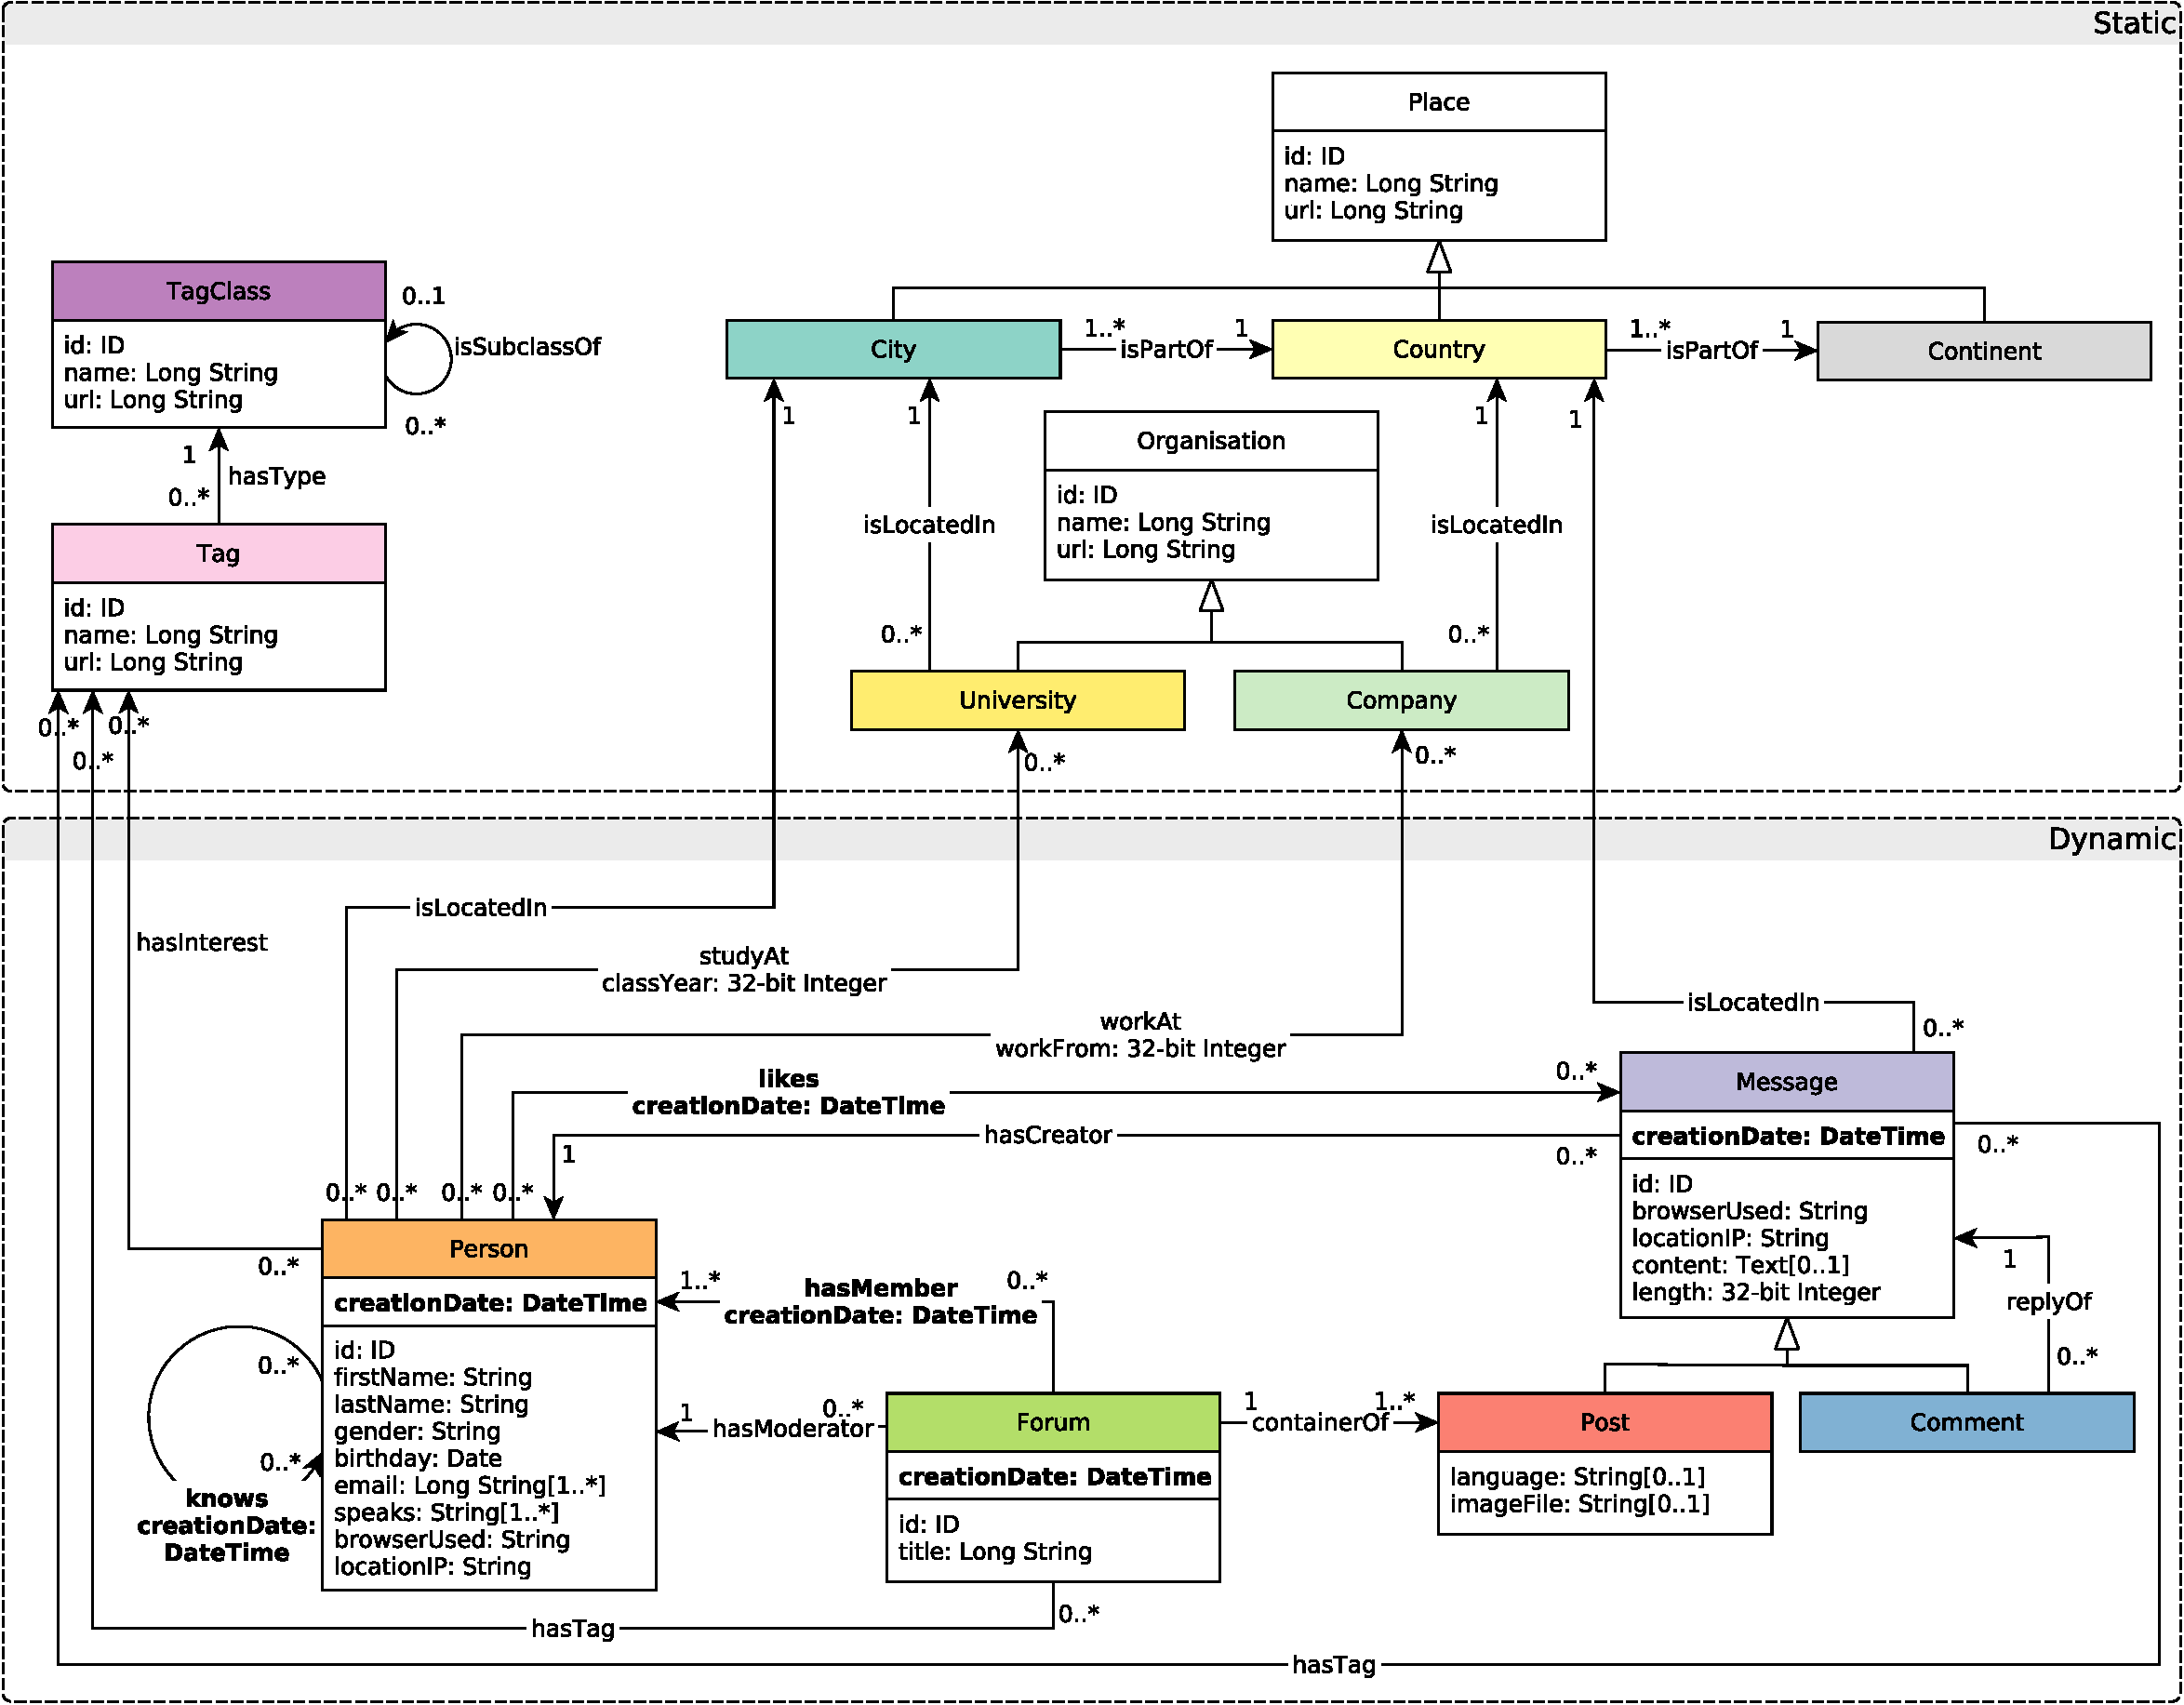
\includegraphics[scale=\yedscale]{figures/schema-comfortable}
    \caption{UML class diagram-style depiction of the \ldbcsnb graph schema. Note that the \textsf{knows} edges should be treated as undirected (but are serialized only in a single direction). The cardinality of the \textsf{hasModerator} edge has changed between version 0.3.x (where it was exactly 1) and version 0.4.x (where it is 0..1).}
    \label{fig:schema}
\end{figure}

The schema specifies different entities, their attributes and their relations.
All of them are described in the following sections.

\subsubsection*{Textual Restrictions and Notes}
\begin{itemize}
    \item Messageas always have a non-empty \texttt{content} attribute.
    \item Posts have either a \texttt{content} or an \texttt{imageFile} attribute (\ie they always have exactly one of them.) The one they do not have is represented with an empty string or with \texttt{NULL}.
    \item Posts in a forum can be created by a non-member person if and only if that person is the moderator of the Forum.
\end{itemize}

\subsection{Entities (nodes)}

{\flushleft \textbf{City:}} a sub-class of a Place, and represents a
city of the real world. City entities are used to specify where persons live,
as well as where universities operate.

{\flushleft \textbf{Comment:}} a sub-class of a Message, and represents a
comment made by a person to an existing message (either a Post or a Comment).

{\flushleft \textbf{Company:}} a sub-class of an Organisation, and represents a company where persons work.

{\flushleft \textbf{Continent:}} a sub-class of a Place, and represents a continent of the real world.

{\flushleft \textbf{Country:}} a sub-class of a Place, and represents a country of the real world.
Countries are selected as the place of operation for Companies as well as the location of Messages.

{\flushleft \textbf{Forum:}} a meeting point where people
post messages. Forums are characterized by the topics (represented as tags)
people in the forum are talking about. Although from the schema's perspective
it is not evident, there exist three different types of
forums.  They are distinguished by their titles:

\begin{itemize}
    \item personal walls: ``Wall of \ldots''
    \item image albums: ``Album $k$ of \ldots''
    \item groups: ``Group for \ldots''
\end{itemize}

\autoref{table:forum} shows the attributes of the Forum entity.

\begin{table}[H]
    \begin{tabular}{|>{\varNameCell}p{\attributeColumnWidth}|>{\typeCell}p{\typeColumnWidth}|p{\descriptionColumnWidth}|}
        \hline
        \tableHeaderFirst{Attribute} & \tableHeader{Type} & \tableHeader{Description} \\
        \hline
        id & ID  & The identifier of the forum.\\
        \hline
        title & Long String  & The title of the forum.\\
        \hline
        creationDate & DateTime  & The date the forum was created.\\
        \hline
    \end{tabular}
    \caption{Attributes of the Forum entity.}
    \label{table:forum}
\end{table}


{\flushleft \textbf{Message:}} an abstract entity that represents a message
created by a person. \autoref{table:message} shows the attributes of the Message
abstract entity.

\begin{table}[H]
    \begin{tabular}{|>{\varNameCell}p{\attributeColumnWidth}|>{\typeCell}p{\typeColumnWidth}|p{\descriptionColumnWidth}|}
        \hline
        \tableHeaderFirst{Attribute} & \tableHeader{Type} & \tableHeader{Description} \\
        \hline
        id & ID  & The identifier of the message.\\
        \hline
        browserUsed & String  & The browser used by the Person to create the message.\\
        \hline
        creationDate & DateTime  & The date the message was created.\\
        \hline
        locationIP & String  & The IP of the location from which the message was created.\\
        \hline
        content & Text (optional)  & The content of the message.\\
        \hline
        length & 32-bit Integer  & The length of the content.\\
        \hline
    \end{tabular}
    \caption{Attributes of the Message interface.}
    \label{table:message}
\end{table}


{\flushleft \textbf{Organisation:}} an institution of the real
world. \autoref{table:organisation} shows the attributes of the Organisation
entity.

\begin{table}[H]
    \begin{tabular}{|>{\varNameCell}p{\attributeColumnWidth}|>{\typeCell}p{\typeColumnWidth}|p{\descriptionColumnWidth}|}
        \hline
        \tableHeaderFirst{Attribute} & \tableHeader{Type} & \tableHeader{Description} \\
        \hline
        id & ID  & The identifier of the organisation.\\
        \hline
        name & Long String  & The name of the organisation.\\
        \hline
        url & Long String  & The URL of the organisation.\\
        \hline
    \end{tabular}
    \caption{Attributes of the Organisation entity.}
    \label{table:organisation}
\end{table}


{\flushleft \textbf{Person:}} the avatar a real world person creates
when he/she joins the network, and contains various information about the
person as well as network related information. \autoref{table:person} shows
the attributes of the Person entity.

\begin{table}[H]
    \begin{tabular}{|>{\varNameCell}p{\attributeColumnWidth}|>{\typeCell}p{\typeColumnWidth}|p{\descriptionColumnWidth}|}
        \hline
        \tableHeaderFirst{Attribute} & \tableHeader{Type} & \tableHeader{Description} \\
        \hline
        id & ID  & The identifier of the person.\\
        \hline
        firstName & String  & The first name of the person.\\
        \hline
        lastName & String  & The last name of the person.\\
        \hline
        gender & String  & The gender of the person.\\
        \hline
        birthday & Date  & The birthday of the person.\\
        \hline
        email & \{Long String\}  & The set of emails the person has (cardinality: at least one).\\
        \hline
        speaks & \{String\}  & The set of languages the person speaks (cardinality: at least one).\\
        \hline
        browserUsed & String  & The browser used by the person when he/she registered to the social network.\\
        \hline
        locationIP & String  & The IP of the location from which the person was registered to the social network.\\
        \hline
        creationDate & DateTime  & The date the person joined the social network.\\
        \hline
    \end{tabular}
    \caption{Attributes of the Person entity.}
    \label{table:person}
\end{table}


{\flushleft \textbf{Place:}} a place in the world.
\autoref{table:place} shows the attributes of the Place entity. Note, each Place has additional parameters: longitude and latitude, which are not exposed. These are used internally for sorting places.

\begin{table}[H]
    \begin{tabular}{|>{\varNameCell}p{\attributeColumnWidth}|>{\typeCell}p{\typeColumnWidth}|p{\descriptionColumnWidth}|}
        \hline
        \tableHeaderFirst{Attribute} & \tableHeader{Type} & \tableHeader{Description} \\
        \hline
        id & ID  & The identifier of the place.\\
        \hline
        name & Long String  & The name of the place.\\
        \hline
        url & Long String  & The URL of the place.\\
        \hline
    \end{tabular}
    \caption{Attributes of the Place entity.}
    \label{table:place}
\end{table}


{\flushleft \textbf{Post:}} a sub-class of Message, that is posted in a
forum. Posts are created by persons into the forums where they belong.
Posts contain either content or imageFile, always one of them but never both.
The one they do not have is an empty string.
\autoref{table:post} shows the attributes of the Post entity.

\begin{table}[H]
    \begin{tabular}{|>{\varNameCell}p{\attributeColumnWidth}|>{\typeCell}p{\typeColumnWidth}|p{\descriptionColumnWidth}|}
        \hline
        \tableHeaderFirst{Attribute} & \tableHeader{Type} & \tableHeader{Description} \\
        \hline
        language & String (optional) & The language of the post. Mutually exclusive with \texttt{imageFile}. \\
        \hline
        imageFile & String (optional) & The image file of the post. Mutually exclusive with \texttt{language}.\\
        \hline
    \end{tabular}
    \caption{Attributes of the Post entity.}
    \label{table:post}
\end{table}


{\flushleft \textbf{Tag:}} a topic or a concept. Tags are used to
specify the topics of forums and posts, as well as the topics a person is
interested in. \autoref{table:tag} shows the atltributes of the Tag entity.

\begin{table}[H]
    \begin{tabular}{|>{\varNameCell}p{\attributeColumnWidth}|>{\typeCell}p{\typeColumnWidth}|p{\descriptionColumnWidth}|}
        \hline
        \tableHeaderFirst{Attribute} & \tableHeader{Type} & \tableHeader{Description} \\
        \hline
        id & ID  & The identifier of the tag.\\
        \hline
        name & Long String  &  The name of the tag.\\
        \hline
        url & Long String  &  The URL of the tag.\\
        \hline
    \end{tabular}
    \caption{Attributes of the Tag entity.}
    \label{table:tag}
\end{table}


{\flushleft \textbf{TagClass:}} a class used to build a hierarchy of tags. \autoref{table:tagclass} shows the attributes of the TagClass entity.

\begin{table}[H]
    \begin{tabular}{|>{\varNameCell}p{\attributeColumnWidth}|>{\typeCell}p{\typeColumnWidth}|p{\descriptionColumnWidth}|}
        \hline
        \tableHeaderFirst{Attribute} & \tableHeader{Type} & \tableHeader{Description} \\
        \hline
        id & ID  & The identifier of the tagclass.\\
        \hline
        name & Long String  &  The name of the tagclass.\\
        \hline
        url & Long String  &  The URL of the tagclass.\\
        \hline
    \end{tabular}
    \caption{Attributes of the TagClass entity.}
    \label{table:tagclass}
\end{table}


{\flushleft \textbf{University:}} a sub-class of Organisation,
and represents an institution where persons study.

\subsection{Relations (edges)}

Relations (edges) connect entities of different types. The endpoint entities are defined by their ``id'' attribute.
Edge instances starting from or ending in a given node are treated as a set, \ie no ordering is defined on the edges.
Multiple edges (\ie edges of the same type between two entity instances) are not allowed in SNB graphs.

\begin{longtable}{|>{\varNameCell}p{2.5cm}|>{\typeCell}p{2.5cm}|>{\typeCell}p{2.5cm}|>{\edgeDirectionCell}c|p{6.5cm}|}
    \hline
     \tableHeaderFirst{Name} & \tableHeader{Source} & \tableHeader{Destination} & \tableHeader{Type} & \tableHeader{Description} \\
     \hline
     containerOf & Forum[1] & Post[0..*] & D & A Forum and a Post contained in it\\
     \hline
     hasCreator & Message[0..*] & Person[1] & D & A Message and its creator (Person)\\
     \hline
     hasInterest & Person[0..*] & Tag[1..*] & D & A Person and a Tag representing a topic the person is interested in\\
     \hline
     hasMember & Forum[0..*] &  Person[1..*] & D & A Forum and its member (Person)

     In version 0.3.x:

     \attributeTable{joinDate}{DateTime}{The Date the person joined the Forum}

     In version 0.4.0+:

     \attributeTable{creationDate}{DateTime}{The Date the person joined the Forum}

     \\
     \hline
     hasModerator & Forum[0..*] &
     \textrm{In version 0.3.x:}
     
     Person[1]
     
     \textrm{In version 0.4.0+:}

     Person[0..1]
     & D & A Forum and its moderator (Person) \\
     \hline
     hasTag & Message[0..*] & Tag[0..*] & D & A Message and a Tag representing the message's topic \\
     \hline
     hasTag & Forum[0..*] & Tag[1..*] & D & A Forum and a Tag representing the forum's topic \\
     \hline
     hasType & Tag[0..*] & TagClass[1] & D & A Tag and a TagClass the tag belongs to \\
     \hline
     isLocatedIn & Company[0..*] & Country[1] & D & A Company and its home Country \\
     \hline
     isLocatedIn & Message[0..*] & Country[1] & D & A Message and the Country from which it was issued \\
     \hline
     isLocatedIn & Person[0..*] & City[1] & D & A Person and their home City \\
     \hline
     isLocatedIn & University[0..*] & City[1] & D &  A University and the City where the university is \\
     \hline
     isPartOf & City[1..*] & Country[1] & D & A City and the Country it is part of \\
     \hline
     isPartOf & Country[1..*] & Continent[1] & D & A Country and the Continent it is part of \\
     \hline
     isSubclassOf & TagClass[0..*] & TagClass[0..1] & D & A TagClass and its parent TagClass \\
     \hline
     knows & Person[0..*] & Person[0..*] & U & Two Persons that know each other.
     Note that
     (1)~the knows edges are undirected (all other edge types are directed and
     (2)~to avoid duplications, these edges are only serialized to one direction and it is the responsibility of the loader/implementation component to treat them as undirected.

     \attributeTable{creationDate}{DateTime}{The date the knows relation was established}

     \\
     \hline
     likes & Person[0..*] & Message[0..*] & D & A Person that likes a Message

     \attributeTable{creationDate}{DateTime}{The date the like was issued}

     \\
     \hline
     replyOf & Comment[0..*] & Message[1] & D & A Comment and the Message it replies \\
     \hline
     studyAt & Person[0..*] & University[0..*] & D & A Person and a University it has studied

     \attributeTable{classYear}{32-bit Integer}{The year the person graduated}

     \\
     \hline
     workAt & Person[0..*] & Company[0..*] & D & A Person and a Company it works

     \attributeTable{workFrom}{32-bit Integer}{The year the person started to work at that Company}

     \\
     \hline
 \caption{Description of the data relations. Type -- \texttt{D}: directed edge, \texttt{U}: undirected edge.}
 \label{table:relations}
\end{longtable}


\subsection{Domain Concepts}

A \emph{thread} consists of Messages, starting with a single Post and the Comments that -- either directly or transitively -- reply to that Post.

\section{Data Generation}
\label{sec:data_generation}

\ldbcsnb provides \datagen (Data Generator), which produces synthetic
datasets following the schema described above. Data
produced mimics a social network's activity during a period of time. Three
parameters determine the generated data: the number of persons, the number of
years simulated, and the starting year of simulation. \datagen is defined by the
following characteristics:

\begin{itemize}
    \item \textbf{Realism.} Data generated by \datagen mimics the
        characteristics of those found in a real social network. In \datagen,
        output attributes, cardinalities, correlations and distributions have
        been finely tuned to reproduce a real social network in each of its
        aspects. On the one hand, it is aware of the  data and link distributions
        found in a real social network such as Facebook. On the other hand, it
        uses real data from DBpedia, such as property dictionaries, which are
        used to ensure that attribute values are realistic and correlated.
    \item \textbf{Scalability.} Since \ldbcsnb targets systems of different
        scales and budgets, \datagen is capable of generating datasets of
        different sizes, from a few Gigabytes to Terabytes. \datagen is
        implemented following the MapReduce parallel paradigm, allowing the
        generation of small datasets in single node machines, as well as large
        datasets on commodity clusters.
    \item \textbf{Determinism.} \datagen is deterministic regardless of the number
        of cores/machines used to produce the data. This important feature
        guarantees that all Test Sponsors will face the same dataset,
        thus, making the comparisons between different systems fair and the
        benchmarks' results reproducible.
    \item \textbf{Usability.} \ldbcsnb is designed to have an affordable entry
        point. As such, \datagen's design is  severely influenced by this
        philosophy, and therefore it is designed to be as easy to use as
        possible.
\end{itemize}


\subsection{Resource Files}

\datagen uses a set of resource files with data
extracted from DBpedia. Conceptually, \datagen generates attribute's
values following a property dictionary model that is defined by

\begin{itemize}
    \item a dictionary $D$
    \item a ranking function $R$
    \item a probability function $F$
\end{itemize}

Dictionary $D$ is a fixed set of values. The ranking function $R$ is a bijection
that assigns to each value in a dictionary a unique rank between 1 and $|D|$.
The probability density function $F$ specifies how the data generator chooses
values from dictionary $D$ using the rank for each term in the dictionary. The
idea to have a separate ranking and probability function is motivated by the
need of generating correlated values: in particular, the ranking function is
typically parameterized by some parameters: different parameter values result
in different rankings. For example, in the case of a dictionary of property
firstName, the popularity of first names might depend on the gender, country
and birthday properties. Thus, the fact that the popularity of first names in
different countries and times is different, is reflected by the different ranks
produced by function $R$ over the full dictionary of names.  \datagen uses a
dictionary for each literal property, as well as ranking functions for all
literal properties. These are materialized in a set of resource files, which
are described in \autoref{table:property_dictionaries}.

\begin{table}[htb]
\begin{tabular}{|p{4cm}|p{12cm}|}
    \hline
    \tableHeaderFirst{Resource Name} & \tableHeader{Description} \\
    \hline
    Browsers & Contains a list of web browsers and their probability to be used. It is used to set the browsers used by the users.\\
    \hline
    Cities by Country & Contains a list of cites and the country they belong. It is used to assign cities to users and universities.\\
    \hline
    Companies by Country & Contains the set of companies per country. It is used to set the countries where companies operate.\\
    \hline
    Countries & Contains a list of countries and their populations. It is used to obtain the amount of people generated for each country.\\
    \hline
    Emails & Contains the set of email providers. It is used to generate the email accounts of persons.\\
    \hline
    IP Zones & Contains the set of IP ranges assigned to each country. It is used to assign the IP addresses to users.\\
    \hline
    Languages by Country & Contains the set of languages spoken in each country. It is used to set the languages spoken by each user.\\
    \hline
    Name by Country & Contains the set of names and the probability to appear in each country. It is used to assign names to persons, correlated with their countries.\\
    \hline
    Popular places by Country & Contains the set of popular places per country. These are used to set where images attached to posts are taken from.\\
    \hline
    Surnames' by Country & Contains the set of surnames and the probability to appear in each country. It is used to assign surnames to persons, correlated with their countries.\\
    \hline
    Tags by Country & Contains a set of tags and their probability to appear in each country. It is used to assign the interests to persons and forums.\\
    \hline
    Tag Classes & Contains, for each tag, the classes it belongs to.\\
    \hline
    Tag Hierarchies & Contains, for each tagClass, their parent tagClass.\\
    \hline
    Tag Matrix & Contains, for each tag, the correlation probability with the other tags. It is used enrich the tags associated to messages.\\
    \hline
    Tag Text & Contains, for each tag, a text. This is used to generate the text for messages.\\
    \hline
    Universities by City & Contains the set of universities per city. It is used to set the cities where universities operate.\\
    \hline
\end{tabular}
\caption{Resource files.}
\label{table:property_dictionaries}
\end{table}


\subsection{Graph Generation}

\autoref{fig:generation_process} conceptually depicts the full data
generation process. The first step loads all the dictionaries and resource
files, and initializes the \datagen parameters.  Second, it generates all the
Persons in the graph, and the minimum necessary information to operate. Part of
this information are the interests of the persons, and the number of knows
relationships of every person, which is guided by a degree distribution
function similar to that found in Facebook~\cite{facebook_anatomy}.

The next three steps are devoted to the creation of knows relationships.  An
important aspect of real social networks, is the fact that similar persons
(with similar interests and behaviors) tend to be connected. This is known as
the Homophily principle~\cite{mcpherson2001birds,DBLP:journals/socnet/BaroneC18}, and implies the presence of
a larger amount of triangles than that expected in a random network. In order
to reproduce this characteristic, \datagen generates the edges by means of
correlation dimensions.  Given a person, the probability to be connected to
another person is typically skewed with respect to some similarity between the
persons. That is, for a person $p$ and for a small set of persons that are
somehow similar to it, there is a high connectivity probability, whereas for
most other persons, this probability is quite low. This knowledge is
exploited by \datagen to reproduce correlations.

\begin{figure}[H]
    \centering
    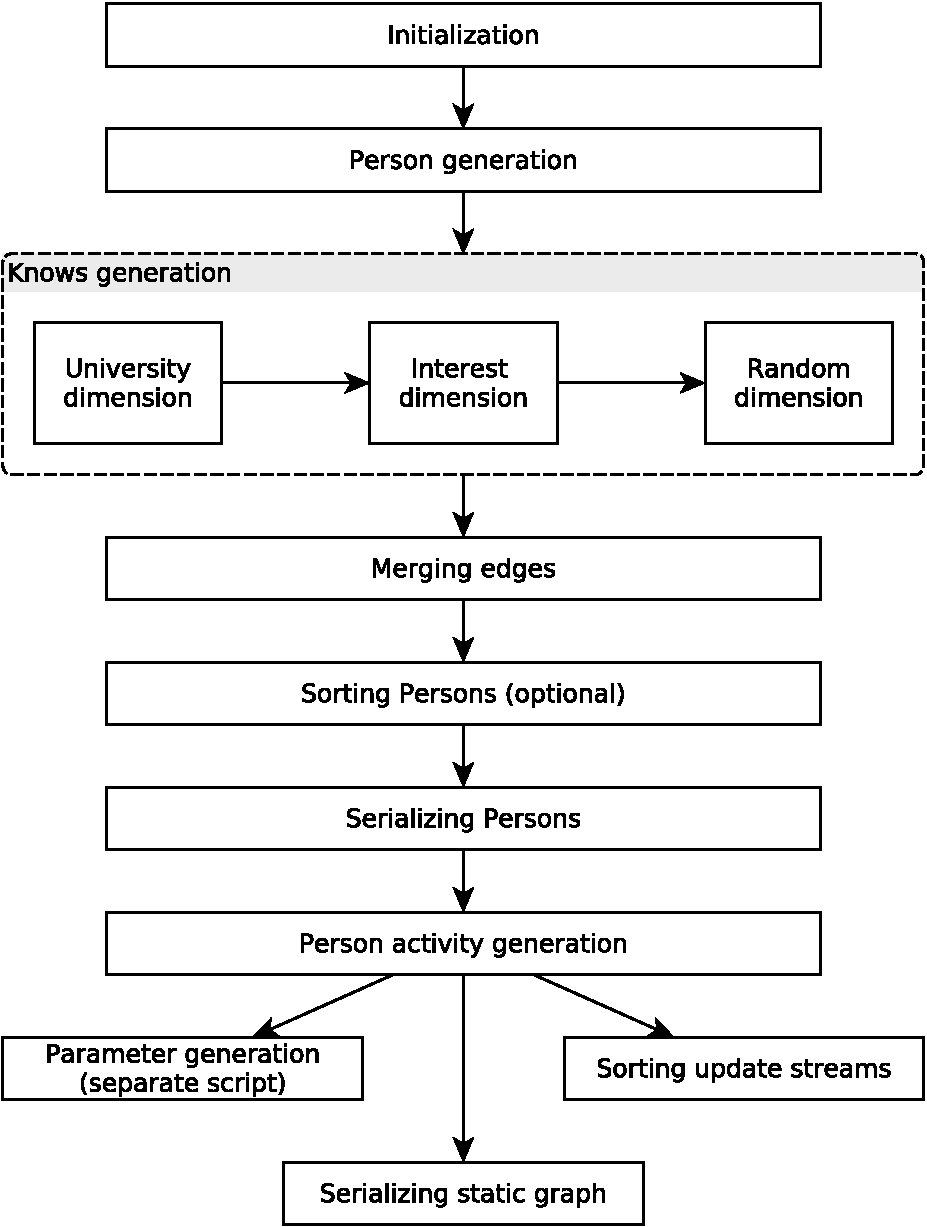
\includegraphics[scale=\yedscale]{figures/datagen-workflow}
    \caption{The \datagen generation process.}
    \label{fig:generation_process}
\end{figure}

Given a similarity function $M(p) : p \rightarrow [0, \infty)$ that gives a score to a person,
with the characteristic that two similar persons will have similar scores, we
can sort all the persons by function $M$ and compare a person $p$ against only the
$K$ neighbouring persons in the sorted array. The consequence of this approach is
that similar persons are grouped together, and the larger the
distance between two persons indicates a monotonic increase in their similarity
difference. In order to choose the persons to connect, \datagen uses a geometric
probability distribution that provides a probability for picking persons to
connect, that are between 1 and $K$ positions apart in the similarity
ranking.

Similarity functions and probability distribution functions over ranked
distance drive what kind of persons will be connected with an edge, not how
many. As stated above, the number of friends of a person is determined by a
Facebook-like distribution. The edges that will be connected to a person $p$,
are selected by randomly picking the required number of edges according to the
correlated probability distributions as discussed before. In the case that
multiple correlations exist, another probability function is used to divide the
intended number of edges between the various correlation dimensions. In \datagen,
three correlated dimensions are chosen: the first one depends on where the
person studied and when, and the second correlation dimension depends on the
interests of the person, and the third one is random (to reproduce the random
noise present in real data). Thus, \datagen has a Facebook-like distributed node
degree, and a predictable (but not fixed) average split between the reasons for
creating edges.

In the next step, a person's activity, in the form of forums, posts and comments
is created. \datagen reproduces the fact that people with a larger number of
friends have a higher activity, and hence post more photos and comments to a
larger number of posts. Another important characteristic of real persons'
activity in social network, are time correlations.  Usually, person' posts
creation in a social network is driven by real world events.  For
instance, one may think about an important event such as the elections in a
country, or a natural disaster. Around the time these events occur, network
activity about these events' topics sees an increase in volume. \datagen
reproduces these characteristics with the simulation of what we name as
flashmob events.  Several events are generated randomly at the beginning of the
generation process, which are assigned a random tag, and are given a time and
an intensity which represents the repercussion of the event in the real world.
When persons' posts are created, some of them are classified as flashmob posts,
and their topics and dates are assigned based on the generated flashmob events.
The volume of activity around this events is modeled following a model similar
to that described in~\cite{DBLP:conf/kdd/LeskovecBKT08}. Furthermore, in order to reproduce the
more uniform every day person activity, \datagen also generates posts uniformly
distributed along all the simulated time.

Finally, in the last step the data is serialized into the output files.

\subsection{Distributions, Parameters and Quirks}
\label{sec:distr-param}

Interesting quirks:
\begin{itemize}
\item A Person is not a member of their Wall but they are its moderator, they do not have a hasMember edge.
\item Each Album generated for Person will have approximately 70\% of their friends as members.
\item A given Person has a 5\% chance of being a moderator of a set of groups.
\item Group membership is composed of 30\% from the moderator's friends and the remainder is chosen randomly (from the block the person is in).
\item Comments are only made in Walls and Groups.
\item Messages can only receive likes during a 7-day window after their creation.
\item Comments always occur within one day of Message they are replying to. The creation date is generated following the power-law distribution in Figure \ref{fig:comments_dist}. The mean delay between Comments and their parent Message is 6.85 hours.
\item Flashmob events span a 72-hour time window with a specific event time in the middle of the window; there are 36 hours each side of the specific event time. Following the distribution in Figure \ref{fig:flashmob_dist} posts are generated either side of flashmob event time, posts are clustered around the specific event time.
\end{itemize}

\begin{figure}[H]
  \centering
  \includegraphics[scale=\yedscale]{figures/comments_power_law}
  \caption{The power-law used to generate comments.}
  \label{fig:comments_dist}
\end{figure}

\begin{figure}[H]
  \centering
  \includegraphics[scale=\yedscale]{figures/flashmob_dist}
  \caption{The distribution used to generate posts during flashmob events.}
  \label{fig:flashmob_dist}
\end{figure}

\subsection{Implementation Details}

\datagen is implemented using the MapReduce parallel paradigm. In MapReduce, a
Map function runs on different parts of the input data, in parallel and on many
node clusters. This function processes the input data and produces for each
result a key. Reduce functions then obtain this data and Reducers run in
parallel on many cluster nodes. The produced key simply determines the Reducer
to which the results are sent. The use of the MapReduce paradigm allows the
generator to scale considerably, allowing the generation of huge datasets by
using clusters of machines.

In the case of \datagen, the overall process is divided into three MapReduce jobs.
In the first job, each mapper generates a subset of the persons of the graph. A
key is assigned to each person using one of the similarity functions described
above. Then, reducers receive the key-value pairs sorted by the key,
generate the knows relations following the described windowing process, and
assign to each person a new key based on another similarity function, for the
next MapReduce pass.  This process can be successively repeated for additional
correlation dimension.  Finally, the last reducer generates the remaining
information such as forums, posts and comments.

\section{Output Data}

For each scale factor, \datagen produces three different artefacts:
\begin{itemize}
  \item \textbf{Dataset:} The dataset to be bulk loaded by the SUT. In the Interactive workload, it corresponds to roughly the 90\% of the total generated network.
  \item \textbf{Update Streams:} A set of update streams containing update
    queries, which are used by the driver to generate the update queries of the
    workloads. This update
    streams correspond to the remaining 10\% of the generated dataset.
  \item \textbf{Substitution Parameters:} A set of files containing the
    different parameter bindings that will be used by the driver to generate the
    read queries of the workloads.
\end{itemize}

\subsection{Scale Factors}
\label{sec:scale-factors}

\ldbcsnb defines a set of scale factors (SFs), targeting systems of different sizes and budgets.
SFs are computed based on the ASCII size \emph{in Gibibytes} of the generated output files using the \textsf{csv-singular-merged-fk} serializer (see \autoref{sec:serializers}).\footnote{This way of characterizing the size of the data set is identical to the scaling of TPC-H and TPC-DS.}
For both workloads, the SF1 data set is 1~GiB, the SF100 is 100~GiB, and the SF\numprint{10000} data set is \numprint{10000} GiB (not 10 TiB).

However, \textbf{note that the two SNB workloads have different data sets} due with different folder structures.

The data sets sizes are established as follows:
For both workloads, we use the default settings for the splitting the data into an intial (bulk-loaded) data set and the later update operations (``streams'').
For Interactive, both the 90\% initial data and the 10\% update streams count towards the total size and the \textsf{csv-singular-merged-fk} serializer is used.
For BI, the sum of the initial snapshot (97\%) and the refresh operations (daily inserts and deletes) are measured and the default CSV serializers (\textsf{composite-merged-fk}) is used.

It is important to note that for a given workload and scale factor, data sets generated using different serializers contain exactly the same data, the only difference is in how they are represented.%
%\footnote{Naturally, there are slight differences in the disk usage of the data sets created with different serializers. For example, for a given scale factor, the disk usage of the data set serialized with the \textsf{csv-singular-projected-fk} serializer is expected to be higher, while with the \textsf{csv-composite-merged-fk}, it is expected to be lower.}

The proposed SFs are the following: 1, 3, 10, 30, 100, 300, \numprint{1000}, \numprint{3000}, \numprint{10000}, \numprint{30000}.
Additionally, three small SFs, 0.003 (for quick tests of data loader components), 0.1, and 0.3 are provided to help initial validation efforts.

The Test Sponsor may select the SF that better fits their needs, by properly configuring the \datagen, as described in \autoref{sec:data_generation}.
The size of the resulting dataset is mainly affected by the following configuration parameters: the number of persons and the number of years simulated.
By default, all SFs are defined over a period of three years, starting from 2010, and SFs are computed by scaling the number of Persons in the network.
\autoref{tab:snsize-bi} shows some metrics of SFs 0.1, \ldots, \numprint{1000} data sets.

\begin{table}[H]
    \small
    \setlength{\tabcolsep}{.5em}
    \centering
    \begin{tabular}{|l||r|r|r|r|r|r|r|r|r|r|r|r|r|r|}
        \hline
        \bf Scale Factor & \bf 0.1 & \bf 0.3 & \bf 1 & \bf 3 & \bf 10 & \bf 30 & \bf 100 & \bf 300 & \bf \numprint{1000} & \bf \numprint{3000} & \bf \numprint{10000} & \bf \numprint{30000} \\ \hline\hline
    \end{tabular}
    \centering
    \caption{Properties of data sets for each scale factor in the BI workload produced by the Spark-based generator. TODO.
        For detailed statistics, see \autoref{tab:number-of-entries-bi}}
    \label{tab:snsize-bi}
\end{table}


%In \autoref{appendix:scale_factors}, we show the statistics of each of the
%proposed SFs in detail, including distributions for some of the relations.

\begin{table}
    \footnotesize
    \centering
    \begin{tabular}{|l|l|c|C{1.2cm}C{1.2cm}|C{1.2cm}C{1.2cm}|}
        \hline
        \multicolumn{1}{|c|}{\multirow{2}{*}{\bf Serializer name (v0.4+)}} & \multicolumn{1}{c|}{\multirow{2}{*}{\bf Legacy serializer name (v0.3)}} & \multirow{2}{*}{\bf Nodes} & \multicolumn{2}{c|}{\bf Attributes} & \multicolumn{2}{c|}{\bf Edges}                                        \\
                                                                           &                                                                         &                            & \bf single-valued                   & \bf multi-valued               & \bf one- to-many & \bf many- to-many \\ \hline
        \texttt{csv-singular-projected-fk}                                 & CsvBasic                                                                & \yes                       & \no                                 & \yes                           & \yes             & \yes              \\
        \texttt{csv-composite-projected-fk}                                & CsvComposite                                                            & \yes                       & \no                                 & \no                            & \yes             & \yes              \\
        \texttt{csv-singular-merged-fk}                                    & CsvMergeForeign                                                         & \yes                       & \no                                 & \yes                           & \no              & \yes              \\
        \texttt{csv-composite-merged-fk}                                   & CsvCompositeMergeForeign                                                & \yes                       & \no                                 & \no                            & \no              & \yes              \\ \hline
    \end{tabular}
    \caption{Attributes and edges serialized to separate files the different CSV serializers.}
    \label{tab:csv-serializers}
\end{table}


\autoref{tab:csv-serializers} shows how each CSV serializer handles attributes/edges of different cardinalities, demonstrating why \textsf{csv-singular-projected-fk} has the most files and \textsf{csv-composite-merged-fk} has the least number of files.

\begin{table}[htb]
    \scriptsize
    \setlength{\tabcolsep}{.5em}
    \centering
    \begin{tabularx}{\linewidth}{|>{\sffamily}c|>{\tt}l|>{\tt}X|}
        \hline
        \tableHeaderFirst{C} & \tableHeader{File}                      & \tableHeader{Content}                                                                                      \\
        \hline\hline
        N                    & static/Organisation/part-*.csv                      & id | type | name | url \\
        E                    & static/Organisation\_isLocatedIn\_Place/part-*.csv  & OrganisationId | PlaceId \\
        \hline
        N                    & static/Place/part-*.csv                             & id | name | url | type \\
        E                    & static/Place\_isPartOf\_Place/part-*.csv            & Place1Id | Place2Id \\
        \hline
        N                    & static/Tag/part-*.csv                               & id | name | url \\
        E                    & static/Tag\_hasType\_TagClass/part-*.csv            & TagId | TagClassId \\
        \hline
        N                    & static/TagClass/part-*.csv                          & id | name | url \\
        E                    & static/TagClass\_isSubclassOf\_TagClass/part-*.csv  & TagClass1Id | TagClass2Id \\
        \hline\hline
        N                    & dynamic/Comment/part-*.csv                          & creationDate | id | locationIP | browserUsed | content | length \\
        E                    & dynamic/Comment\_hasCreator\_Person/part-*.csv      & creationDate | CommentId | PersonId \\
        E                    & dynamic/Comment\_hasTag\_Tag/part-*.csv             & creationDate | CommentId | TagId \\
        E                    & dynamic/Comment\_isLocatedIn\_Country/part-*.csv    & creationDate | CommentId | CountryId \\
        E                    & dynamic/Comment\_replyOf\_Comment/part-*.csv        & creationDate | Comment1Id | Comment2Id \\
        E                    & dynamic/Comment\_replyOf\_Post/part-*.csv           & creationDate | CommentId | PostId \\
        \hline
        N                    & dynamic/Forum/part-*.csv                            & creationDate | id | title \\
        E                    & dynamic/Forum\_containerOf\_Post/part-*.csv         & creationDate | ForumId | PostId \\
        E                    & dynamic/Forum\_hasMember\_Person/part-*.csv         & creationDate | ForumId | PersonId \\
        E                    & dynamic/Forum\_hasModerator\_Person/part-*.csv      & creationDate | ForumId | PersonId \\
        E                    & dynamic/Forum\_hasTag\_Tag/part-*.csv               & creationDate | ForumId | TagId \\
        \hline
        N                    & dynamic/Person/part-*.csv                           & creationDate | id | firstName | lastName | gender | birthday | locationIP | browserUsed | language | email \\
        E                    & dynamic/Person\_hasInterest\_Tag/part-*.csv         & creationDate | personId | interestId \\
        E                    & dynamic/Person\_isLocatedIn\_City/part-*.csv        & creationDate | PersonId | CityId \\
        E                    & dynamic/Person\_knows\_Person/part-*.csv            & creationDate | Person1Id | Person2Id \\
        E                    & dynamic/Person\_likes\_Comment/part-*.csv           & creationDate | PersonId | CommentId \\
        E                    & dynamic/Person\_likes\_Post/part-*.csv              & creationDate | PersonId | PostId \\
        E                    & dynamic/Person\_studyAt\_University/part-*.csv      & creationDate | PersonId | UniversityId | classYear \\
        E                    & dynamic/Person\_workAt\_Company/part-*.csv          & creationDate | PersonId | CompanyId | workFrom \\
        \hline
        N                    & dynamic/Post/part-*.csv                             & creationDate | id | imageFile | locationIP | browserUsed | language | content | length \\
        E                    & dynamic/Post\_hasCreator\_Person/part-*.csv         & creationDate | PostId | PersonId \\
        E                    & dynamic/Post\_hasTag\_Tag/part-*.csv                & creationDate | PostId | TagId \\
        E                    & dynamic/Post\_isLocatedIn\_Country.csv              & creationDate | PostId | CountryId \\
        \hline
    \end{tabularx}
    \caption{Files output by the \texttt{csv-composite-projected-fk} serializer (31 in total). The first part of the table contains the static entites, the second part contains the dynamic ones.
        Notation -- \textsf{C}: entity category, \textsf{N}: node, \textsf{E}: edge.}
    \label{table:csv-composite-projected-fk}
\end{table}


\begin{table}[htb]
    \scriptsize
    \centering
    \begin{tabularx}{\linewidth}{|>{\sffamily}c|>{\tt}l|>{\tt}X|}
        \hline
        \tableHeaderFirst{C} & \tableHeader{File}                   & \tableHeader{Content}                                                                                               \\
        \hline\hline
        N                    & static/Organisation/part-*.csv                   & id | type | name | url | LocationPlaceId \\
        \hline
        N                    & static/Place/part-*.csv                          & id | name | url | type | PartOfPlaceId \\
        \hline
        N                    & static/Tag/part-*.csv                            & id | name | url | TypeTagClassId \\
        \hline
        N                    & static/TagClass/part-*.csv                       & id | name | url | SubclassOfTagClassId \\
        \hline\hline
        N                    & dynamic/Comment/part-*.csv                       & creationDate | id | locationIP | browserUsed | content | length | CreatorPersonId | LocationCountryId | ParentPostId | ParentCommentId \\
        E                    & dynamic/Comment\_hasTag\_Tag/part-*.csv          & creationDate | CommentId | TagId \\
        \hline
        N                    & dynamic/Forum/part-*.csv                         & creationDate | id | title | ModeratorPersonId \\
        E                    & dynamic/Forum\_hasMember\_Person/part-*.csv      & creationDate | ForumId | PersonId \\
        E                    & dynamic/Forum\_hasTag\_Tag/part-*.csv            & creationDate | ForumId | TagId \\
        \hline
        N                    & dynamic/Person/part-*.csv                        & creationDate | id | firstName | lastName | gender | birthday | locationIP | browserUsed | LocationCityId | language | email \\
        E                    & dynamic/Person\_hasInterest\_Tag/part-*.csv      & creationDate | personId | interestId \\
        E                    & dynamic/Person\_knows\_Person/part-*.csv         & creationDate | Person1Id | Person2Id \\
        E                    & dynamic/Person\_likes\_Comment/part-*.csv        & creationDate | PersonId | CommentId \\
        E                    & dynamic/Person\_likes\_Post/part-*.csv           & creationDate | PersonId | PostId \\
        E                    & dynamic/Person\_studyAt\_University/part-*.csv   & creationDate | PersonId | UniversityId | classYear \\
        E                    & dynamic/Person\_workAt\_Company/part-*.csv       & creationDate | PersonId | CompanyId | workFrom \\
        \hline
        N                    & dynamic/Post/part-*.csv                          & creationDate | id | imageFile | locationIP | browserUsed | language | content | length | CreatorPersonId | ContainerForumId | LocationCountryId \\
        E                    & dynamic/Post\_hasTag\_Tag/part-*.csv             & creationDate | PostId | TagId \\
        \hline
    \end{tabularx}
    \caption{Files output by the \texttt{csv-composite-merged-fk} serializer (18 in total). The first part of the table contains the static entites, the second part contains the dynamic ones.
        Notation -- \textsf{C}: entity category, \textsf{N}: node, \textsf{E}: edge.}
    \label{table:csv-composite-merged-fk}
\end{table}


\begin{table}[htb]
    \scriptsize
    \centering
    \begin{tabularx}{\linewidth}{|>{\sffamily}c|>{\tt}l|>{\tt}X|}
        \hline
        \tableHeaderFirst{C} & \tableHeader{File}                   & \tableHeader{Content}                                                                                                                                                                    \\
        \hline\hline
        N                    & static/Organisation/part-*.csv                   & id | type | name | url | LocationPlaceId \\
        \hline
        N                    & static/Place/part-*.csv                          & id | name | url | type | PartOfPlaceId \\
        \hline
        N                    & static/Tag/part-*.csv                            & id | name | url | TypeTagClassId \\
        \hline
        N                    & static/TagClass/part-*.csv                       & id | name | url | SubclassOfTagClassId \\
        \hline\hline
        N                    & dynamic/Comment/part-*.csv                       & creationDate | deletionDate | explicitlyDeleted | id | locationIP | browserUsed | content | length | CreatorPersonId | LocationCountryId | ParentPostId | ParentCommentId \\
        E                    & dynamic/Comment\_hasTag\_Tag/part-*.csv          & creationDate | deletionDate | CommentId | TagId \\
        \hline
        N                    & dynamic/Forum/part-*.csv                         & creationDate | deletionDate | explicitlyDeleted | id | title | ModeratorPersonId \\
        E                    & dynamic/Forum\_hasMember\_Person/part-*.csv      & creationDate | deletionDate | explicitlyDeleted | ForumId | PersonId \\
        E                    & dynamic/Forum\_hasTag\_Tag/part-*.csv            & creationDate | deletionDate | ForumId | TagId \\
        \hline
        N                    & dynamic/Person/part-*.csv                        & creationDate | deletionDate | explicitlyDeleted | id | firstName | lastName | gender | birthday | locationIP | browserUsed | LocationCityId | language | email \\
        E                    & dynamic/Person\_hasInterest\_Tag/part-*.csv      & creationDate | deletionDate | personId | interestId \\
        E                    & dynamic/Person\_knows\_Person/part-*.csv         & creationDate | deletionDate | explicitlyDeleted | Person1Id | Person2Id \\
        E                    & dynamic/Person\_likes\_Comment/part-*.csv        & creationDate | deletionDate | explicitlyDeleted | PersonId | CommentId \\
        E                    & dynamic/Person\_likes\_Post/part-*.csv           & creationDate | deletionDate | explicitlyDeleted | PersonId | PostId \\
        E                    & dynamic/Person\_studyAt\_University/part-*.csv   & creationDate | deletionDate | PersonId | UniversityId | classYear \\
        E                    & dynamic/Person\_workAt\_Company/part-*.csv       & creationDate | deletionDate | PersonId | CompanyId | workFrom \\
        \hline
        N                    & dynamic/Post/part-*.csv                          & creationDate | deletionDate | explicitlyDeleted | id | imageFile | locationIP | browserUsed | language | content | length | CreatorPersonId | ContainerForumId | LocationCountryId \\
        E                    & dynamic/Post\_hasTag\_Tag/part-*.csv             & creationDate | deletionDate | PostId | TagId \\
        \hline
    \end{tabularx}
    \caption{Directories created by the raw serializer (18 in total). The first part of the table contains the static entites, the second part contains the dynamic ones.
        Notation -- \textsf{C}: entity category, \textsf{N}: node, \textsf{E}: edge.
        The entities with the \texttt{explicitlyDeleted} attribute -- Comment, Forum, Post nodes, and hasMember, knows, likes (Comment/Post) edges -- denote whether the entity is deleted as part of an explicit delete operation or implicitly through a cascading delete operation.}
    \label{table:csv-raw}
\end{table}


\subsection{Serializers}
\label{sec:serializers}

The datasets are generated in the \texttt{social\_network/} directory, split into static and dynamic parts (\autoref{fig:schema}).
The filenames (without the extension) end in \texttt{\_i\_j} where \texttt{i} is the block id and \texttt{j} is the partition id (set by \texttt{numThreads}).
The SUT has to take care only of the generated Dataset to be bulk loaded. Using \texttt{NULL} values for storing optional values is allowed.

\datagen currently only supports CSV-based serializers.
These produce CSV-like text files which use the pipe character ``\texttt{|}'' as the primary field separator and the semicolon character ``\texttt{;}'' as a separator for multi-valued attributes (for the composite serializers).
The CSV files are stored in two subdirectories: \texttt{static/} and \texttt{dynamic/}.
Depending on the number of threads used for generating the dataset, the number of files varies, since there is a file generated per thread. We indicate this with ``\texttt{part-*}'' in the specification.

The following CSV variants are supported:
    \begin{itemize}
      \item \textsf{csv-composite-projected-fk:}
      Each relation with a cardinality larger than one are output in a separate file.
      Generated files are summarized in \autoref{table:csv-composite-projected-fk}.

      \item \textsf{csv-composite-merged-fk:}
      This serializer is similar to \textsf{csv-composite-projected-fk}, but relations that have a cardinality of 1-to-N are merged in the entity files as a foreign keys.
      There are 13~such relations in total:
      \begin{itemize}
        \item Comment\_hasCreator\_Person, Comment\_isLocatedIn\_Country, Comment\_replyOf\_Comment, Comment\_replyOf\_Post (merged to Comment);
        \item Forum\_hasModerator\_Person (merged to Forum);
        \item Organisation\_isLocatedIn\_Place (merged to Organisation);
        \item Person\_isLocatedIn\_City (merged to Person);
        \item Place\_isPartOf\_Place (merged to Place);
        \item Post\_hasCreator\_Person, Post\_isLocatedIn\_Country, Forum\_containerOf\_Post (merged to Post);
        \item Tag\_hasType\_TagClass (merged to Tag);
        \item TagClass\_isSubclassOf\_TagClass (merged to TagClass)
      \end{itemize}
      Generated files are summarized in \autoref{table:csv-composite-merged-fk}.
    
      \item \textsf{csv-singular-merged-fk}:
      Similar to the \textsf{csv-composite-merged-fk} but multi-valued attributes (\texttt{Person.email} and \texttt{Person.speaks}) are stored as separate directories (\texttt{Person\_email\_EmailAddress} and \texttt{Person\_speaks\_Language}, resp.).
    
      \item \textsf{csv-singular-projected-fk}:
      Similar to the \textsf{csv-composite-projected-fk} but multi-valued attributes (\texttt{Person.email} and \texttt{Person.speaks}) are stored as separate directories (\texttt{Person\_email\_EmailAddress} and \texttt{Person\_speaks\_Language}, resp.).

      \item \texttt{raw} mode:
      The file names are the same as in \texttt{composite-merged-fk} but there are two important differences:
      (1)~additional attributes, \eg \texttt{deletionDate}, \texttt{explicitlyDeleted}, and \texttt{weight} (used for weighted graphs in Graphalytics~\cite{DBLP:journals/corr/abs-2011-15028}), are included,
      (2)~all data is included, \ie if a Forum is created and deleted before sampling the initial data set, it is included in this data set.
      Generated files are summarized in \autoref{table:csv-raw}.
    \end{itemize}

The inheritance hierarchies in the schema have two important characteristics
(1)~all subclasses use the same id space, \eg there cannot be a Comment and a Post with id 1 at the same time,
(2)~they are serialized to CSVs using either the \emph{map hierarchy to single table} or \emph{map each concrete class to its own table} strategies\footnote{\url{http://www.agiledata.org/essays/mappingObjects.html}}:

\begin{description}
    \item[Message = Comment | Post]
    \emph{Map each concrete class to its own table} is used \ie separate CSV files are used for the Comment and the Post classes.

    \item[Place = City | Country | Continent]
    \emph{Map hierarchy to single table} is used, \ie all Place node are serialized in a single file. A discriminator attribute ``type'' is used with the value denoting the concrete class, \eg ``Country''.

    \item[Organisation = Company | University]
    \emph{Map hierarchy to single table} is used, \ie all Organisation nodes are serialized in a single fiel. A discriminator attribute ``type'' is used with the value denoting the concrete class, \eg ``Company''.
\end{description}

\subsection{Interactive Update Streams (inserts)}

The generic schema for the Interactive update streams is given in \autoref{table:update_stream_generic_schema}, while the concrete schemas of each insert operations is given in \autoref{table:update_stream_schemas}.
The update stream files are generated in the \texttt{social\_network/} directory and are grouped as follows:

\begin{itemize}
    \item \texttt{updateStream\_*\_person.csv} files contain update operation 1: \queryRefCard{interactive-insert-01}{INS}{1}
    \item \texttt{updateStream\_*\_forum.csv} files contain update operations 2--8: %
    \queryRefCard{interactive-insert-02}{INS}{2}
    \queryRefCard{interactive-insert-03}{INS}{3}
    \queryRefCard{interactive-insert-04}{INS}{4}
    \queryRefCard{interactive-insert-05}{INS}{5}
    \queryRefCard{interactive-insert-06}{INS}{6}
    \queryRefCard{interactive-insert-07}{INS}{7}
    \queryRefCard{interactive-insert-08}{INS}{8}
\end{itemize}

Remark: update streams in version 0.3.0 only contain inserts. Delete operations are being designed and will be released later.

\subsection{Substitution Parameters}

The substitution parameters are generated in the \texttt{substitution\_parameters/} directory.
Each parameter file is named \texttt{\{interactive|bi\}\_<id>\_param.txt}, corresponding to an operation of
Interactive complex reads (\queryRefCard{interactive-complex-read-01}{IC}{1}--\queryRefCard{interactive-complex-read-14}{IC}{14}) and
BI reads (\queryRefCard{bi-read-01}{BI}{1}--\queryRefCard{bi-read-20}{BI}{20}).
The schemas of these files are defined by the operator, \eg the schema of \queryRefCard{interactive-complex-read-01}{IC}{1} is ``\texttt{personId|firstName}''.

%%%%%%%%%%%%%%%%%%%%%%%%%%%%%%%%%%%%%%%%%%%%%%%%%%%%%%%%%%%%%%%%%%%%%%%%%%%%%%
%%%%%%%%%%%%%%%%%%%%%%%%%%%%%%%%%%%%%%%%%%%%%%%%%%%%%%%%%%%%%%%%%%%%%%%%%%%%%%
%%%%%%%%%%%%%%%%%%%%%%%%%%%%%%%%%%%%%%%%%%%%%%%%%%%%%%%%%%%%%%%%%%%%%%%%%%%%%%

\section{Introducing Delete Operations}

\paragraph{Challenge for systems}
To support deletion operations graph processing systems need to solve numerous technical challenges:
%
\begin{enumerate}
\item Users should be able to \emph{express deletion operations} using the database API, preferably using a high-level declarative query language with clear semantics~\cite{Green2019}.
\item Deletion operations \emph{limit the algorithms and data structures} that can be used by a system. Certain dynamic graph algorithms are significantly more expensive to recompute in the presence of deletes~\cite{DBLP:conf/soda/Roditty13} or only support either insert or deletions but not both~\cite{DBLP:conf/esa/RodittyZ04}. A number of updatable matrix storage formats only support efficient insertions but not deletions~\cite{DBLP:conf/hpec/BusatoGBB18}. Meanwhile some graph databases might be able to exploit indices to speed up deletions~\cite[Sec.~4.4.2]{Besta2019}
\item \emph{Distributed graph databases} need to employ specialized protocols to enforce consistency of deletions~\cite{Waudby2020}.
\end{enumerate}

\paragraph{Challenge for benchmarks}
Due to their importance and challenging nature, we found it necessary to incorporate delete operations into LDBC benchmarks.
However, doing so is a non-trivial task as it impacts on each component in the benchmark workflow:
workload specifications, data generation, parameter curation, and the workload driver.
This section focuses primarily data generation.

The initial step in generating delete operations is to define the semantics of the desired operations.
To understand common behaviour of deletes we informally surveyed several social networks, the findings of which motivated the design
of 8 delete operations described in~\autoref{sec:bi-refreshes}.

The next step was to generate \emph{delete events} within LDBC's synthetic data generator and ensure that they follow a logic order in
the social network.
For example, a delete \tKnows edge event can only occur after both \tPersons join the network and become friends,
but before either \tPerson leaves the network.
To achieve this Datagen was extended to support \emph{dynamic entities}.
Dynamic entities have a \emph{creation date} and a \emph{deletion date}, which together comprise an entity's \emph{lifespan}.
Once generated this allows for the extraction of deletion operations, which can be utilized by LDBC workloads.
Deriving valid lifespans for dynamic entities was the subject of a short paper published at the GRADES-NDA~2020
workshop~\cite{DBLP:conf/sigmod/WaudbySPS20} and is presented in~\autoref{sec:lifespan-management}.

Next it was important to distinguish between \emph{implicit} and \emph{explicit} delete events.
Continuing with the \tKnows edge example, once created the connection exists until either \tPerson leaves the network,
at which point the connection is implicitly deleted, as per the semantics of delete \tPerson~(\autoref{sec:bi-delete-01}).
Alternatively, at any time up until this event, the friendship can be explicitly deleted,
\ie two people have a disagreement and ``unfriend'' each other, but both continue using the social network.
Distinguishing between these types of events is important as only explicit delete events should become delete operations
in the workload.

To achieve this each dynamic entity is assigned a probability of being explicitly deleted, if selected the entity is marked as such;
this is used to ensure the correct serialization of delete events into delete operations.
For entities selected for explicit deletion the next step is to determine a realistic time at which the event occurs.
For example, a post has a higher probability of being deleted soon after it was posted compared to after 5 days.
To achieve this each dynamic entity is assigned a realistic distribution to select delete event timestamps from,
which respects the bounds imposed by the valid lifespans.
The probability distributions used to determine if a dynamic entities is explicitly deleted and then when that event occurs is discussed
in~\autoref{sec:ensuring-realism}.

Once generated dynamic entities must be correctly serialized.
Depending on its creation date, deletion date, and if the entity is explicitly deleted it can,
(i) spawn an insert and delete operation,
(ii) be included in the bulk load component and spawn a delete operation,
(iii) just be included in the bulk load component,
(iv) spawn only an insert operation, and
(v) not be serialized at all!
The approach for doing this is presented in~\autoref{sec:conv-delete-events}.

We summarize the numerous challenges supporting the generation of dynamic entities and thus delete operations poses below:
\begin{enumerate}
\item \textbf{Validity.} The generator should produce \emph{valid lifespans},
where each generated dynamic entity guarantees that
(a)~events in the graph follow a logical order: \eg in a social network, two people can become friends only after both persons joined the network and before either person leaves the network,
(b)~the graph never violates the cardinality constraints prescribed by its schema, and
(c)~the graph continuously satisfies the semantic constraints required by the application domain (\eg no isolated comments in a social network).
\item \textbf{Realism.} The generator should create a graph with a realistic correlations and distribution of entities over time.
For example, in a social network the distribution of activity is non-uniform over time, real-world events such as elections or controversial posts %by celebrities
can drive spikes of posts and unfollowings respectively~\cite{DBLP:conf/www/MyersL14}.
In addition, deletions can be correlated with certain attributes: \eg the likelihood a person leaves the network may be correlated with their number of friends~\cite{Lorincz2019}.
Also, there are often temporal correlations between entity creation and deletion: \eg posts have an increased chance of deletion immediately following creation compared to after a 3~month period.
\item \textbf{Serialization.} Care must be taken to distinguish between implicit and explicit delete events when creating the bulk load component, insert operations, and delete operations.
\item \textbf{Scalability.} A graph with dynamic entities should be generated at scale (up to billions of edges).
\end{enumerate}

%%% [JACK: commented out]
% \subsection{Challenge}

% \paragraph{Deletions in graph generators}

% Supporting deletions within graph generators poses numerous challenges.
% First, they should produce \emph{valid deletions},
% where each generated deletion operation guarantees that
% (a)~the entity targeted for deletion exists at the time of the execution of the operation (even when multiple deletion operations are executed concurrently),
% (b)~the graph never violates the cardinality constraints prescribed by its schema, and
% (c)~the graph continuously satisfies the semantic constraints required by the application domain (\eg no isolated comments in a social network).
% Second, deletions should be generated at scale (up to billions of edges).
% % our solution: building on top of LDBC Datagen -- this uses a Hadoop implementation, which 'scales'
% Third, they should create a graph with a realistic distribution of entities over time.
% For example, in a social network it is reasonable to assume that events do not follow a uniform distribution but there are a number of bursty events.


% Moreover, the probability of a given entity in the
% We intend to specify deletion probabilities for each entity in the graph.
% That is, the probability a given entity is explicitly deleted in simulation period.
% This probability may be a function of several attributes.
% For example, the probability a person leaves the network is a function of their number of connections -- the more friends, more social capital and less likely to leave.
% A second dimension we intend to consider is the distribution within the intervals.
% For example, if a post is selected for deletion, the interval we sample from may not be uniformly distributed.
% Posts may have a higher chance of deletion straight after they have been posted rather than 3 months after they have been posted or if other posts have already been deleted.
% Thirdly, it would be interesting to model flashmob-like unfollowings/deletions, a famous person posts a racist tweet for example

% [Gabor] the "VaSCo properties" -- valid, scalable, correlated
% valid
% scalable (future work = Datagen migration)
% correlations, flash delete (future work)

\section{Lifespan Management}
\label{sec:lifespan-management}

This section is based on the short paper published at the GRADES-NDA~2020 workshop~\cite{DBLP:conf/sigmod/WaudbySPS20} authored by the task force members.

%Such are generated from the intervals below, which capture the dependencies between entities. For example, a \tPost cannot be created until the \tPerson that creates that message, joins the network, the forum is created and the \tPerson joins the \tForum.

In this section, we define the constraints for generating dynamic entities in a social network. Each dynamic entity gets a \emph{lifespan}, represented by two \emph{lifespan attributes}, a \emph{creation date} and a \emph{deletion date}.
% Entities exist in the network within this lifespan.
We first briefly review the data generator, introduce our notation and define the parameters of the generation process. Then, we define the semantic constraints which regulate the participation in certain relationships along with the constraints for selecting intervals. We illustrate an application of these with two examples, shown in \autoref{fig:example-graph} and \autoref{fig:example-graph-complex}.

\paragraph{Graph schema}

The LDBC Datagen component~\cite{Pham2012,Datagen} is responsible for generating the graph used in the benchmarks. It produces a synthetic dataset modelling a social network's activity. Its graph schema has 11~concrete node types connected by 20~edge types, and its entities (nodes/edges) are classified as either dynamic or static (\autoref{fig:schema}).
The dynamic part of the graph comprises of a fully connected \tPerson graph and a number of \tMessage trees under \tForums.

\paragraph{Notation}
To describe lifespans and related constraints, we use the following notation.
Constants are uppercase bold, \eg $\constant{NC}$.
Entity types are monospaced, \eg \tPerson, \tHasMember.
Variables are lowercase italic, \eg $\variable{pers}, \variable{hm}$.
Entities are sans-serif, \eg $\instance{P_1}, \instance{HM}$.
For an entity $x$, $\varc{x}{}$ denotes its creation date, while $\vard{x}{}$ denotes its deletion date.
In most cases, both the creation and the deletion date are selected from an interval, \eg $\varc{x}{} \in \interval{d_1}{d_2}$ means that entity $\variable{x}$ should be created between dates $d_1$ (inclusive) and $d_2$ (exclusive).
The selected creation and deletion dates together form an interval that represents the lifespan of its entity.
If any of the intervals for selecting the lifespan attributes of an entity are empty, \ie $d_2 \leq d_1$, the entity should be discarded.
As illustrated later, this interval is often used to determine the intervals where the creation and deletion dates of dependant entities are selected.

\paragraph{Parameters} % maybe comes later?
We parameterize the generator as follows.
The network is created in 2010 and exists for 10~years at which point the network collapses ($\xNC = 2020$).
Data is simulated for a 3-year period, between the simulation start, $\xSS = 2010$ and the simulation end, $\xSE = 2013$.
In order to allow \emph{windowed execution} by the LDBC SNB driver (used for multi-threaded and distributed operation), we define a sufficiently large amount of time that needs to pass between consecutive operations on an entity as $\Delta = 10\text{s}$.

%\paragraph{Examples}
%\autoref{fig:example-graph} shows an example illustrating the lifespans of two $\type{\tPerson}$ nodes and a $\type{knows}$ edge.
%A complex example that includes $\type{Forum}$, $\type{Post}$ and $\type{Comment}$ nodes is shown in  \autoref{fig:example-graph-2}.

\subsection{General Rules}

In this section, we define general rules that must be satisfied by all entities in the graph. In subsequent sections, we refine these with domain-specific constraints.
For a node $\varn{1}$, we always require that:
\begin{itemize}
    \item $\varcn{1} \in \interval{\xSS}{\xSE}$, the node must be created between the simulation start and the simulation end.
    \item $\vardn{1} \in \interval{\varcn{1} + \Delta}{\xNC}$, the node must exist for at least $\Delta$ time and must be deleted before the network collapse.
\end{itemize}


To enforce referential integrity constraints (\ie prevent dangling edges), the lifespan of edge $\variable{e}$ between nodes $\varn{1}$ and $\varn{2}$ must always satisfy the following criteria:

\begin{itemize}
    \item $ \varc{e} \in \interval
        {\max(\varcn{1}, \varcn{2})}
        {\min(\vardn{1}, \vardn{2}, \xSE)} $,
        in other terms,
        the edge must be created no sooner than both of its endpoints
        but before
        any of its endpoints are deleted.
        %creation date of and edge must be larger than or equal to those of its endpoints.
    \item $ \vard{e} \in \interval
        {\varc{e} + \Delta}
        {\min(\vardn{1}, \vardn{2})} $,
        \ie the edge must exist for at least $\Delta$ time and
        deleted no later than
        any of its endpoints.
\end{itemize}

To further refine the constraints for edges, we distinguish between two main cases.

(1)~The endpoints of edge $\variable{e}$ are existing node $\varn{1}$ and node $\varn{2}$ which is inserted at the same time as the edge:
\begin{itemize}
    \item $ \varc{e} = \varcn{2} $ % \quad (we know that $\varcn{1} \geq \varcn{2} + \Delta$)
    \item $ \vard{e} = \min(\vardn{1}, \vardn{2}) $.
    In case of edges with \emph{containment semantics} (node $\varn{1}$ contains $\varn{2}$ through edge $e$),
    node $\varn{2}$ must always be deleted at the same time as edge $\variable{e}$,
    therefore
    $\vard{e} = \vardn{2}$ and $\vardn{2} \leq \vardn{1}$.
    %
%\footnote{We require each entity to exist for at least $\Delta$ time, so $\vardn{1} \geq \varcn{1} + \Delta $. Therefore, given $\varc{e} = \varcn{1}$, assigning $\vard{e} = \vardn{1}$ confirms $ \vard{e} \in \interval{\varc{e} + \Delta}{\min(\vardn{1}, \vardn{2})}$.}
\end{itemize}

(2)~In other cases, the edge must be created when both of its endpoints already exist and must be deleted no later than them:

\begin{itemize}
    \item $ \varc{e} \in \interval
        {\max(\varcn{1}, \varcn{2}) + \Delta}
        {\min(\vardn{1}, \vardn{2}, \xSE)} $
    \item $ \vard{e} \in \interval
        {\varc{e} + \Delta}
        {\min(\vardn{1}, \vardn{2})} $
\end{itemize}

These constraints capture the ``minimum'' (\ie most relaxed) set of constraints that must be enforced in all domains.
Next, we introduce additional constraints specific to our social network schema.

\subsection{Person}

A \tPerson $\ePerson$ is the avatar a real-world person creates when they join the network. A \tPerson joins the network, $\varc{\ePerson}$, during the simulation period and they leave the network, $\vard{\ePerson}$, during the network lifetime:
%provided the following conditions hold:

\begin{itemize}
    \item $\varc{\ePerson} \in \interval{\xSS}{\xSE}$
    \item $\vard{\ePerson} \in \interval{\varc{\ePerson} + \Delta}{\xNC}$
\end{itemize}
%When most users leave a network they do so without deleting their profiles; around 22\% explicitly delete their profiles~\cite{Lorincz2019}. Also, the probability of a given \tPerson leaving the network varies depending on the amount of \emph{social capital} they stand to lose~\cite{Lorincz2019}. Social capital is the utility an individual gains from human interaction, this is captured at a coarse-grain by the number of connections an individual has in the network - \tPersons with higher \tKnows  degrees are less willing leave the network as they have more social capital to lose. These two phenomenon are captured when $\vard{\ePerson}$ is selected from the above interval.

For the edges of \tPerson nodes pointing to a static node
($\type{isLocatedIn}$,
$\type{studyAt}$,
$\type{workAt}$, and
$\type{hasInterest}$),
we assign the creation and deletion date from $\varc{\ePerson}$ and $\vard{\ePerson}$, resp.

% \begin{itemize}
% \item maybe make creation date non-uniform across simulation period? Or we assume the network is in the middle of its life?
% \item when probability of deletion based on connection distribution has been defined should we include it?
% \end{itemize}

%\input{figures/graph-person-knows}
\begin{figure}[ht]
  \centering
  \begin{subfigure}{\linewidth}
    \tikzstyle{vertex} = [circle,minimum width=45pt,draw]
    \centering
    \begin{tikzpicture}[node distance=2cm]
      \node (v1) [vertex,xshift=0cm,yshift=0cm,fill=Person] {\scriptsize{$\instance{P_1}:\type{Person}$}};
      \node (v2) [vertex,xshift=5cm,yshift=0cm,fill=Person] {\scriptsize{$\instance{P_2}:\type{Person}$}};
      \node [below of=v1,yshift=1cm] {\tiny{\texttt{$\instc{P}{1}$: Feb 22 2010}}};
      \node [below of=v1,yshift=0.7cm] {\tiny{\texttt{$\instd{P}{1}$: Jul 26 2014}}};
      \node [below of=v2,yshift=1cm] {\tiny{\texttt{$\instc{P}{2}$: Mar 07 2010}}};
      \node [below of=v2,yshift=0.7cm] {\tiny{\texttt{$\instd{P}{2}$: Oct 17 2012}}};
      \draw[thick,->,>=stealth] (v1) --
      node [midway,above] {\scriptsize{$\instance{knows_{1,2}} : \type{Knows}$}}
      node [midway,below,align=right,text width=2.5cm] {\tiny{\texttt{$\instc{knows}{1,2}$: Dec 01 2011}}}
      node [midway,below,yshift=-0.3cm,align=right,text width=2.5cm] {\tiny{\texttt{$\instd{knows}{1,2}$: Jun 05 2012}}} (v2);
    \end{tikzpicture}
    \caption{An instance of a \tKnows edge connecting two \tPerson nodes. \emph{Creation} and \emph{deletion} dates are shown for each entity.}
    \label{fig:person-knows-graph}
    \end{subfigure}
  %
    \begin{subfigure}{\linewidth}
    \footnotesize
    \centering
    \begin{tikzpicture}[node distance=2cm,thick,every node/.style={transform shape}]
      %\tikzset{grid/.style={grey,very thin,opacity=1}} \draw[grid] (-3,0/1.5) grid (9,-6/1.5);

      \draw [thick,->,>=stealth] node [above,black] {} (-1,0/1.5) -- (6,0/1.5); % timeline
      \draw [grey,thin] (-0.5,0/1.5) node [above,black] {$\xSS$} -- (-0.5,-6/1.5);
      \draw [grey,thin]  (5.5,0/1.5) node [above,black] {$\xNC$} -- (5.5,-6/1.5);
      \draw [grey,thin]  (4.5,0/1.5) node [above,black] {$\xSE$} -- (4.5,-6/1.5);

      %P_1
      \draw[mark=*,mark size=2pt,mark options={color=green}] plot coordinates {(0.5,-1/1.5)} node [left] {$\instance{P_1}$}
      -- plot[mark=*,mark size=2pt,mark options={color=red}] coordinates {(5.0,-1/1.5)};

      %P_2
      \draw[mark=*,mark size=2pt,mark options={color=green}] plot coordinates {(1,-2/1.5)}  node [left] {$\instance{P_2}$}
      -- plot[mark=*,mark size=2pt,mark options={color=red}] coordinates {(4.0,-2/1.5)};

      % knows-c
      \draw[thin,grey,<->] plot coordinates {(1.3,-3/1.5)} node [left,black,xshift=-0.2cm] {\textcolor{grey}{$\instc{knows}{1,2}$}} node [align=right,xshift=-3.2cm,text width=2.55cm] {{\textcolor{green}{$\max(\instc{P}{1}, \instc{P}{2}) + \Delta$}}}
      -- plot[mark=*,mark size=2pt,mark options={color=blue}] coordinates {(2.5,-3/1.5)}
      -- plot coordinates {(4.0,-3/1.5)} node [xshift=3cm,text width=2.5cm] {{\textcolor{red}{$\min(\instd{P}{1}, \instd{P}{2}, \xSE)$}}};

     \draw [grey,thin,dashed] (4.0,-2/1.5) -- (4.0,-3/1.5);
     \shadedBox(1,-2/1.5,1/1.5);


     % knows-d
     \draw[thin,grey,<->] plot coordinates {(2.8,-4/1.5)} node [left,black,xshift=-0.2cm] {\textcolor{grey}{$\instd{knows}{1,2}$}} node [align=right,xshift=-4.7cm,text width=2.55cm] {{\textcolor{green}{$\instc{knows}{1,2} + \Delta$}}}
     -- plot[mark=*,mark options={color=blue}] coordinates {(3.5,-4/1.5)}
     -- plot coordinates {(4.0,-4/1.5)} node [xshift=3cm,text width=2.5cm] {{\textcolor{red}{$\min (\instd{P}{1},  \instd{P}{2})$}}}; %, \xNC

     \draw [grey,thin,dashed] (4.0,-3/1.5) -- (4.0,-4/1.5);
     \shadedBox(2.5,-3/1.5,1/1.5);

     % knows
      \draw[mark=*,mark size=2pt,mark options={color=green}] plot coordinates {(2.5,-5/1.5)}  node [left] {$\instance{knows_{1,2}}$}
      -- plot[mark=*,mark size=2pt,mark options={color=red}] coordinates {(3.5,-5/1.5)};
     \draw [thin,dashed,grey] (2.5,-4/1.5) -- (2.5,-5/1.5);
     \draw [thin,dashed,grey] (3.5,-4/1.5) -- (3.5,-5/1.5);

    \end{tikzpicture}
    \caption{
      Illustration of the intervals in which the \emph{creation} \textcolor{green}{$\bullet$} and \emph{deletion} \textcolor{red}{$\bullet$} dates can be selected.
      Thick black lines represent entity lifespans and thin grey lines represent valid intervals that dates can be selected in; \textcolor{blue}{$\bullet$} indicates the selected times (spanning the lifespan interval of the given entity).
      On the thin grey lines, thicker sections represent the minimal amount of time that must pass before selecting a value.
      In case of creation dates, this is used to ensure that the dependant entity exists for at least $\Delta$ time.
      In case of deletion dates, it is used to ensure that the entity exists for at least $\Delta$ time.
    }
    \label{fig:person-knows}
  \end{subfigure}

  \caption{Example graph and its intervals.}
  \label{fig:example-graph}
\end{figure}


\subsubsection{Knows}

The \tKnows edge connects two \tPersons $p_i$ and $p_j$ that know each other in the network.
%When assigning \tKnows a creation date and deletion date the lifespans of the \tPersons being connected must be carefully considered, as both \tPersons must exist in the network at some point in time for them to connect.
The intervals where the creation and deletion dates can be generated in are illustrated in \autoref{fig:person-knows} and defined below:
\begin{itemize}
    \item $\varc{\eKnows_{i,j}} \in \interval{\max(\varc{\ePerson}_{i},\varc{\ePerson}_{j}) + \Delta}{\min(\vard{\ePerson}_{i},\vard{\ePerson}_{j}, \xSE)}$
    \item $\vard{\eKnows_{i,j}} \in \interval{\varc{\eKnows_{i,j}} + \Delta}{\min (\vard{\ePerson}_{i}, \vard{\ePerson}_{j})}$
\end{itemize}


\subsection{Forum and Message}

The rules for \tForum and \tMessage nodes along with their edges are given in \autoref{sec:forum} and \autoref{sec:message}, respectively, and illustrated in \autoref{fig:example-graph-complex}.


% \begin{figure*}[ht]
%   \centering
%   \includegraphics[width=\textwidth]{figures/degree-average-through-time-white}
%   \caption{Average $\type{know}$ degree for $\type{Person}$s in the network, measured once per day throughout the simulation period. For each scale factor, measurements were taken on four graphs built from the generated updates varying the deletions included. Experiment repeated across Scale Factors 1, 10, and 30.}
%   \label{fig:degrees}
% \end{figure*}

\subsection{Forum}
\label{sec:forum}
\label{sec:hasModerator}

A \tForum is a meeting point where people post \tMessages.
There exists three categories of \tForums:
Wall ($\eForum_\textsf{w}$),
Album ($\eForum_\textsf{a}$),
and Group ($\eForum_\textsf{g}$).
Each \tForum has a set of \tPersons connected via \tHasMember edges, a set of \tTags connected via \tHasTag edges, a single moderator connected by a \tHasModerator edge and a set of \tMessages (discussed in Section \ref{sec:message}).
For all \tForums the outgoing \tHasTag edges get their creation date and deletion date from $\varc{\eForum}$ and $\vard{\eForum}$, respectively.

\subsubsection{Groups}
Groups are public places for people that share interests, any \tPerson can create a Group $\eForum_\textsf{g}$ during their lifespan. A Group can be deleted anytime after it was created.
\begin{itemize}
    \item $\varc{\eForum}_{\mathsf{g}} \in \interval{\varc{\ePerson} + \Delta}{\min (\vard{\ePerson}, \xSE)}$
    \item $\vard{\eForum}_{\mathsf{g}} \in \interval{\varc{\eForum}_{\mathsf{g}} + \Delta}{\xNC}$
\end{itemize}

\paragraph{Group Moderator}
The initial \tHasModerator $\eHasModerator_{\mathsf{g}}$ is the Group creator. If the moderator leaves the Group, the Group will have no moderator (this is allowed in the schema of version 0.4.0+, see \autoref{fig:schema}).
\begin{itemize}
\item $\varc{\eHasModerator}_{\mathsf{g}} \in \interval{\varc{\eForum}_{\mathsf{g}} + \Delta}{\min (\vard{\eForum}_{\mathsf{g}}, \vard{\ePerson}, \xSE)}$
\item $\vard{\eHasModerator}_{\mathsf{g}} \in \interval{ \varc{\eHasModerator}_{\mathsf{g}} + \Delta}{\min (\vard{\eForum}_{\mathsf{g}}, \vard{\ePerson})}$
\end{itemize}

\paragraph{Group Membership}
Any \tPerson $\ePerson$ can become a member of a given group. The \tHasMember $\eHasMember_{\mathsf{g}}$ creation is generated from the interval in which the \tPerson and \tForum lifespans overlap. The deletion date is generated from the interval between the membership creation date (incremented by $\Delta$) and the minimum of the \tPerson and \tForum deletion dates.
\begin{itemize}
    \item $\varc{\eHasMember}_{\mathsf{g}} \in \interval{\max ( \varc{\eForum}_{\mathsf{g}}, \varc{\ePerson}) + \Delta}{\min (\vard{\eForum}, \vard{\ePerson}, \xSE)} $
    \item $\vard{\eHasMember}_{\mathsf{g}} \in \interval{\varc{\eHasMember}_{\mathsf{g}} + \Delta}{\min (\vard{\eForum}_{\mathsf{g}}, \vard{\ePerson})}$
\end{itemize}

\subsubsection{Walls}
Every \tPerson $\ePerson$, has a Wall $\eForum_\textsf{w}$ which is created when the \tPerson joins the social network. The wall is deleted when the \tPerson is deleted.
\begin{itemize}
    \item $\varc{\eForum}_{\mathsf{w}} = \varc{\ePerson} + \Delta$
    \item $\vard{\eForum}_{\mathsf{w}} = \vard{\ePerson}$
\end{itemize}

\paragraph{Wall Moderator}
Each \tPerson has a \tHasModerator $\eHasModerator_{\mathsf{w}}$ edge to their wall, which gets the creation date (incremented by $\Delta$) and deletion date from $\eForum_\textsf{w}$.
Note, only the moderator can create \tPost nodes on the wall and the connecting \tTag nodes are set based on the interest of the moderator.
\begin{itemize}
    \item $\varc{\eHasModerator}_{\mathsf{w}} = \varc{\eForum}_{\mathsf{w}} + \Delta$
    \item $\vard{\eHasModerator}_{\mathsf{w}} = \vard{\eForum}_{\mathsf{w}}$
\end{itemize}

\paragraph{Wall Membership}
For a \tPerson $p_i$, all their friends $p_j$ (\tPerson nodes connected via a \tKnows edge) become members of $\eForum_\textsf{w}$ at the time the \tKnows edge is created. Hence, a \tHasMember $\eHasMember_{\mathsf{w}}$ edge gets the creation date of \tKnows incremented by $\Delta$. The deletion date is derived from the minimum of the \tForum deletion date and \tKnows deletion date.
\begin{itemize}
    \item $\varc{\eHasMember}_{\mathsf{w}} = \varc{\eKnows_{i,j}} + \Delta$
    \item $\vard{\eHasMember}_{\mathsf{w}} = \min(\vard{\eForum}_{\mathsf{w}}, \vard{\eKnows_{i,j}})$
\end{itemize}

\subsubsection{Albums}
A \tPerson can create multiple Albums ($\eForum_\textsf{a}$) containing a set of \tPhotos{}. Albums can be created and then deleted at any point during the lifespan of the \tPerson.
\begin{itemize}
    \item $\varc{\eForum}_\textsf{a} \in \interval{\varc{\ePerson} + \Delta}{\min (\vard{\ePerson}, \xSE)}$
    \item $\vard{\eForum}_\textsf{a} \in \interval{ \varc{\eForum}_\textsf{a} + \Delta}{\vard{\ePerson}}$
\end{itemize}

\paragraph{Album Moderator}
The \tPerson is the moderator for any Album they create. Album ownership cannot change hence \tHasModerator $\eHasModerator_{\mathsf{a}}$ gets the creation date (incremented by $\Delta$) and deletion date from $\varc{\eForum}_\textsf{a}$ and $\vard{\eForum}_\textsf{a}$ respectively.
\begin{itemize}
\item $\varc{\eHasModerator}_{\mathsf{a}} = \varc{\eForum}_{\mathsf{a}} + \Delta$
\item $\vard{\eHasModerator}_{\mathsf{a}} = \vard{\eForum}_{\mathsf{a}}$
\end{itemize}

\paragraph{Album Membership}
Only friends $\ePerson_i$ of a \tPerson $\ePerson_j$ can become members of Albums created by $\ePerson_j$. The \tHasMember $\eHasMember_{\mathsf{a}}$ edge creation date is derived from the Album and $\type{knows}$ creation dates. The deletion is derived from the $\type{Forum}$ and $\type{knows}$ deletion dates.
\begin{itemize}
    \item $\varc{\eHasMember}_\textsf{a} = \max ( \varc{\eForum}_\textsf{a}, \varc{\eKnows}_{i,j} ) + \Delta $
    \item $\vard{\eHasMember}_{\mathsf{w}} = \min ( \vard{\eForum}_\textsf{a}, \vard{\eKnows}_{i,j} ) $
\end{itemize}

\subsection{Message}
\label{sec:message}

A \tMessage is an abstract entity that represents a message created by a \tPerson.
There are two \tMessage subtypes: \tPost and \tComment.
A \tPost is created in a \tForum and a \tComment represents a comment made by a \tPerson to an existing \tMessage (either a \tPost or a \tComment).
In a \tForum the set of \tMessage nodes form a \emph{tree} with a \tPost node at the root and \tComment nodes for the rest.

\subsubsection{Post}

A \tPost can be created by a \tPerson in a \tForum.
Only the moderator (\ie owner) can post on a Wall or in an Album (\tHasModerator),
whereas all members including the moderator (\tHasMember/\tHasModerator) can post in a Group.
These relationships are captured with the $\eHasMember$ variable in the formulas.
\tPosts are divided in three categories, \emph{regular posts}, \emph{photos}, and \emph{flashmob posts}.

\paragraph{Regular Posts and Photos}

Regular posts capture the standard daily activity in a Group or on a Wall.
Photos are created in Albums. (Interaction with Photos is limited to \tLikes, see details in \autoref{sec:likes}). The creation date for these is determined as follows:
$$\varc{\ePost} \in \interval{\varc{\eHasMember} + \Delta}{\min (\vard{\eHasMember}, \xSE) }$$

\paragraph{Flashmob Posts}

Flashmob posts are generated around events that attract significant interest
(such as elections) that result in a spike in activity.
These events span a $2\phi$-hour time window centered around a specific event time, flashmob event $\eFlashmobEvent$, in the middle of the window; there are $\phi$ hours each side of the specific event time.
$$
\varc{\ePost} \in \interval{\max(\varc{\eHasMember} + \Delta,\eFlashmobEvent - \phi\textrm{\,h})}{\min (\vard{\eHasMember},\eFlashmobEvent + \phi\textrm{\,h},\xSE)}
$$

The deletion dates for all categories of \tPosts are determined as:
$$\vard{\ePost} \in \interval{\varc{\ePost} + \Delta}{\vard{\eHasMember}}$$

\paragraph{containerOf edge}

Each \tPost node has an incoming $\type{containerOf}$ edge which gets the same lifespan attributes as the \tPost.

\subsubsection{Comment}

A \tComment $\eComment$ is created by \tPerson $\ePerson$ as a reply to \tMessage $\eMessage$. \tComments are only made in Walls and Groups. \tComment always occur within $\gamma$~days of their parent message following a power-law distribution with mean 6.85 hours.

\begin{itemize}
    \item $\varc{\eComment} \in \interval{\max (\varc{\eMessage}, \varc{\eHasMember}) + \Delta}{\min (\varc{\eMessage} + \gamma\textrm{\,d}, \vard{\eHasMember}, \xSE)}$
    \item $\vard{\eComment} \in \interval{\varc{\eComment} + \Delta}{\min (\vard{\eMessage}, \vard{\eHasMember})}$
\end{itemize}

\paragraph{replyOf edge}

\tComments always have an outgoing \tReplyOf edge with containment semantics, \ie the target \tMessage contains the \tComment. These edges get the same lifespan as their source \tComment.

\subsubsection{likes}
\label{sec:likes}

A \tLikes edge $\eLikes$ can exist between \tPerson $\ePerson$ and \tMessage $\eMessage$. Messages can only receive likes during a $\mu$-day window after their creation at which point no more activity is generated.

\begin{itemize}
    \item $\varc{\eLikes} \in \interval{\max(\varc{\ePerson}, \varc{\eMessage}) + \Delta}{\min (\vard{\ePerson}, \vard{\eMessage}, \varc{\eMessage} + \mu\textrm{\,d}, \xSE)}$
    \item $\vard{\eLikes} \in \interval{\varc{\eLikes} + \Delta}{\min (\vard{\ePerson}, \vard{\eMessage})}$
\end{itemize}

\subsection{Complex Example}
\label{sec:complex-example}

In \autoref{fig:example-graph-complex}, a complex example graph is shown with the corresponding intervals.
Both \emph{the intervals for selecting the creation and deletion date} attributes and the selected \emph{lifespan intervals} are shown.

\begin{figure*}[htp]
  \centering
  \begin{subfigure}{\linewidth}
    \input{figures/fig-comments-graph}
    \caption{Example graph with an instance of a \tForum containing a \tMessage tree of depth 3 and its \tPerson members. Lifespan attributes (\emph{creation} and \emph{deletion dates}) are shown for each dynamic entity. Edges in grey get their lifespan attributes as per \autoref{fig:schema} and \autoref{sec:hasModerator}.}
    \label{fig:comments-graph}
  \end{subfigure}
  %
  \begin{subfigure}{\linewidth}
    \centering
    \footnotesize
    \begin{tikzpicture}[node distance=2cm,thick,scale=0.78,every node/.style={transform shape}]
      % timeline
      \draw [thick,->,>=stealth] node [above,black] {} (-1,0/1.8) -- (13,0/1.8);
      \draw [grey,thin] (-0.5,0/1.8) node [above,black] {$\xSS$} -- (-0.5,-22/1.8);
      \draw [grey,thin] (12.5,0/1.8) node [above,black] {$\xNC$} -- (12.5,-22/1.8);
      \draw [grey,thin] (11.8,0/1.8) node [above,black] {$\xSE$} -- (11.8,-22/1.8);

      % P_1
      \draw[mark=*,mark size=2pt,mark options={color=green}] plot coordinates {(0.5,-1/1.8)} node [left] {$\instance{P_1}$}
      -- plot[mark=*,mark size=2pt,mark options={color=red}] coordinates {(12,-1/1.8)};
      \shadedBox(0.5,-1/1.8,1/1.8);

      % forum^c_{g,1}
      \draw[thin,grey,<->] plot coordinates {(0.8,-2/1.8)} node [left,black,xshift=-0.2cm] {\textcolor{grey}{$\instc{F}{1}$}} node [align=right,xshift=-3.5cm,text width=4cm] {{\textcolor{green}{$\instc{P}{1} + \Delta$}}}
      -- plot[mark=*,mark size=2pt,mark options={color=blue}] coordinates {(1,-2/1.8)}
      -- plot coordinates {(11.8,-2/1.8)} node [xshift=3.0cm,text width=4cm] {{\textcolor{red}{$\min(\instd{P}{1},\xSE)$}}};
      \shadedBox(1,-2/1.8,1/1.8);

      % forum^d_{g,1}
      \draw[thin,grey,<->] plot coordinates {(1.3,-3/1.8)} node [left,black,xshift=-0.2cm] {\textcolor{grey}{$\instd{F}{1}$}} node [align=right,xshift=-4cm,text width=4cm] {{\textcolor{green}{$\instc{F}{1} + \Delta$}}}
      -- plot[mark=*,mark size=2pt,mark options={color=blue}] coordinates {(11,-3/1.8)}
      -- plot coordinates {(12.5,-3/1.8)} node [xshift=2.3cm,text width=4cm] {{\textcolor{red}{$\xNC$}}};
      \draw [grey,thin,dashed] (1,-3/1.8) -- (1,-4/1.8);
      \draw [grey,thin,dashed] (11,-3/1.8) -- (11,-4/1.8);

      % F_{g,1}
      \draw[mark=*,mark size=2pt,mark options={color=green}] plot coordinates {(1,-4/1.8)}  node [left] {$\instance{F_{1}}$}
      -- plot[mark=*,mark size=2pt,mark options={color=red}] coordinates {(11,-4/1.8)};
      \draw [thin,dashed,grey]   (1.0,-4/1.8) -- (1,-5/1.8);

      \draw [thin,dashed,gray] (2.5,-4/1.8) -- (2.5,-9/1.8);
      \draw [thin,dashed,gray] (10.5,-4/1.8) -- (10.5,-11/1.8);
      \draw [thin,dashed,gray]   (11.0,-4/1.8) -- (11,-7/1.8);

      % P_2
      \draw[mark=*,mark size=2pt,mark options={color=green}] plot coordinates {(0.2,-5/1.8)}  node [left] {$\instance{P_2}$}
      -- plot[mark=*,mark size=2pt,mark options={color=red}] coordinates {(11.25,-5/1.8)};
      \shadedBox(1,-5/1.8,1/1.8)

      % hasMember^c_{g,2}
      \draw[thin,grey,<->] plot coordinates {(1.3,-6/1.8)} node [left,black,xshift=-0.2cm] {\textcolor{grey}{$\instc{HM}{2}$}} node [align=right,xshift=-4cm,text width=4cm] {{\textcolor{green}{{$\max ( \instc{F}{1}, \instc{P}{2}) + \Delta$}}}}
      -- plot[mark=*,mark size=2pt,mark options={color=blue}] coordinates {(1.7,-6/1.8)}
      -- plot coordinates {(11,-6/1.8)} node [xshift=3.8cm,text width=4cm] {{\textcolor{red}{$\min(\instd{F}{1},\instd{P}{2},\xSE)$}}};
      \shadedBox(1.7,-6/1.8,1/1.8);

      % hasMember^d_{g,2}
      \draw[thin,grey,<->] plot coordinates {(2,-7/1.8)} node [left,black,xshift=-0.2cm] {\textcolor{grey}{$\instd{HM}{2}$}} node [align=right,xshift=-4.7cm,text width=4cm] {{\textcolor{green}{$\instc{HM}{2} + \Delta$}}}
      -- plot[mark=*,mark size=2pt,mark options={color=blue}] coordinates {(10.7,-7/1.8)}
      -- plot coordinates {(11,-7/1.8)} node [xshift=3.8cm,text width=4cm] {{\textcolor{red}{$\min(\instd{F}{1}, \instd{P}{2})$}}};
      \draw [grey,thin,dashed] (1.7,-7/1.8) -- (1.7,-8/1.8);
      \draw [grey,thin,dashed] (10.7,-7/1.8) -- (10.7,-8/1.8);

      % HM_{g,2}
      \draw[mark=*,mark size=2pt,mark options={color=green}] plot coordinates {(1.7,-8/1.8)}  node [left] {$\instance{HM_{2}}$}
      -- plot[mark=*,mark size=2pt,mark options={color=red}] coordinates {(10.7,-8/1.8)};

      % P_3
      \draw[mark=*,mark size=2pt,mark options={color=green}] plot coordinates {(2.5,-9/1.8)}  node [left] {$\instance{P_3}$}
      -- plot[mark=*,mark size=2pt,mark options={color=red}] coordinates {(10.5,-9/1.8)};
      \shadedBox(2.5,-9/1.8,1/1.8);

      % hasMember^c_{g,3}
      \draw[thin,grey,<->] plot coordinates {(2.8,-10/1.8)} node [left,black,xshift=-0.2cm] {\textcolor{grey}{$\instc{HM}{3}$}}
      -- plot[mark=*,mark size=2pt,mark options={color=blue}] coordinates {(3.5,-10/1.8)} node [align=right,xshift=-6.2cm,text width=4cm] {{\textcolor{green}{{$\max ( \instc{F}{1}, \instc{P}{3}) + \Delta$}}}}
      -- plot coordinates {(10.5,-10/1.8)} node [xshift=4.3cm,text width=4cm] {{\textcolor{red}{$\min(\instd{F}{1}, \instd{P}{3}, \xSE)$}}};
      \shadedBox(3.5,-10/1.8,1/1.8);

      % hasMember^d_{g,3}
      \draw[thin,grey,<->] plot coordinates {(3.8,-11/1.8)} node [left,xshift=-0.2cm,black] {\textcolor{grey}{$\instd{HM}{3}$}} node [align=right,xshift=-6.5cm,text width=4cm] {{\textcolor{green}{$\instc{HM}{3} + \Delta$}}}
      -- plot[mark=*,mark size=2pt,mark options={color=blue}] coordinates {(10,-11/1.8)}
      -- plot coordinates {(10.5,-11/1.8)} node [xshift=4.3cm,text width=4cm] {{\textcolor{red}{$\min(\instd{F}{1}, \instd{P}{3})$}}};
      \draw [grey,thin,dashed] (3.5,-11/1.8) -- (3.5,-12/1.8);
      \draw [grey,thin,dashed] (10,-11/1.8) -- (10,-12/1.8);

      % HM_{g_3}

      \draw[mark=*,mark size=2pt,mark options={color=green}] plot coordinates {(3.5,-12/1.8)}  node [left] {$\instance{HM_{3}}$}
      -- plot[mark=*,mark size=2pt,mark options={color=red}] coordinates {(10,-12/1.8)};
      \shadedBox(3.5,-12/1.8,1/1.8);
      \draw [thin,dashed,grey] (10,-12/1.8)  -- (10,-14/1.8);

      % post^c_{g,3}
      \draw[thin,grey,<->] plot coordinates {(3.8,-13/1.8)} node [left,black,xshift=-0.2cm] {\textcolor{grey}{$\instc{Post}{1}$}} node [align=right,xshift=-6.5cm,text width=4cm] {{\textcolor{green}{{$\instc{HM}{3} + \Delta$}}}}
      -- plot[mark=*,mark size=2pt,mark options={color=blue}] coordinates {(4,-13/1.8)}
      -- plot coordinates {(10,-13/1.8)} node [xshift=4.8cm,text width=4cm] {{\textcolor{red}{$\min (\instd{HM}{3}, \xSE)$}}};
      \shadedBox(4,-13/1.8,1/1.8);

      % post^d_{g,3}
      \draw[thin,grey,<->] plot coordinates {(4.3,-14/1.8)} node [left,black,xshift=-0.2cm] {\textcolor{grey}{$\instd{Post}{1}$}} node [align=right,xshift=-7cm,text width=4cm] {{\textcolor{green}{$\instc{Post}{1} + \Delta$}}}
      -- plot[mark=*,mark size=2pt,mark options={color=blue}] coordinates {(9.5,-14/1.8)}
      %-- plot coordinates {(10,-14/1.8)} node [xshift=4.8cm,text width=4cm] {{\textcolor{red}{$\min (\instd{HM}{3})$}}}; %, \xNC
      -- plot coordinates {(10,-14/1.8)} node [xshift=4.8cm,text width=4cm] {{\textcolor{red}{$\instd{HM}{3}$}}}; %, \xNC
      \draw [grey,thin,dashed] (4,-14/1.8) -- (4,-15/1.8);
      \draw [grey,thin,dashed] (9.5,-14/1.8) -- (9.5,-15/1.8);

      % Post_{3}
      \draw[mark=*,mark size=2pt,mark options={color=green}] plot coordinates {(4,-15/1.8)}  node [left] {$\instance{Post_1}$}
      -- plot[mark=*,mark size=2pt,mark options={color=red}] coordinates {(9.5,-15/1.8)};
      \draw [thin,dashed,grey] (5.3,-15/1.8)  -- (5.3,-16/1.8);

      % comment^c_{g,1}
      \draw[thin,grey,<->] plot coordinates {(4.3,-16/1.8)} node [left,black,xshift=-0.2cm] {\textcolor{grey}{$\instc{C}{1}$}} node [align=right,xshift=-7cm,text width=4cm] {{\textcolor{green}{{$\max (\instc{Post}{1}, \instc{HM}{1}) + \Delta$}}}}
      -- plot[mark=*,mark size=2pt,mark options={color=blue}] coordinates {(4.8,-16/1.8)}
      -- plot coordinates {(5.3,-16/1.8)} node [xshift=9.5cm,text width=4cm] {{\textcolor{red}{$\min (\instc{Post}{1} + \gamma\,\mathrm{d}, \instd{HM}{1}, \xSE)$}}};
      \shadedBox(4,-15/1.8,1/1.8);

      % comment^d_{g,1}
      \draw[thin,grey,<->] plot coordinates {(5.1,-17/1.8)} node [left,black,xshift=-0.2cm] {\textcolor{grey}{$\instd{C}{1}$}} node [align=right,xshift=-7.8cm,text width=4cm] {{\textcolor{green}{{$\instc{Post}{1} + \Delta$}}}}
      -- plot[mark=*,mark size=2pt,mark options={color=blue}] coordinates {(7.8,-17/1.8)}
      -- plot coordinates {(9.5,-17/1.8)} node [xshift=5.3cm,text width=4cm] {{\textcolor{red}{$\min (\instd{Post}{1}, \instd{HM}{1})$}}}; %,\xNC
      \draw [grey,thin,dashed] (4.8,-17/1.8) -- (4.8,-18/1.8);
      \draw [grey,thin,dashed] (7.8,-17/1.8) -- (7.8,-18/1.8);

      \shadedBox(4.8,-16/1.8,1/1.8);
      \draw [thin,dashed,grey] (9.5,-15/1.8)  -- (9.5,-17/1.8);

      % C_{1}
      \draw[mark=*,mark size=2pt,mark options={color=green}] plot coordinates {(4.8,-18/1.8)}  node [left] {$\instance{C_1}$}
      -- plot[mark=*,mark size=2pt,mark options={color=red}] coordinates {(7.8,-18/1.8)};

      % comment^c_{g,2}
      \draw[thin,grey,<->] plot coordinates {(5.1,-19/1.8)} node [left,black,xshift=-0.2cm] {\textcolor{grey}{$\instc{C}{2}$}} node[align=right,xshift=-7.8cm,text width=4cm] {{\textcolor{green}{{$\max (\instc{C}{1}, \instc{HM}{2}) + \Delta$}}}}
      -- plot[mark=*,mark size=2pt,mark options={color=blue}] coordinates {(5.5,-19/1.8)}
      -- plot coordinates {(6.1,-19/1.8)}  node [xshift=8.7cm,text width=4cm] {{\textcolor{red}{$\min (\instc{C}{1} + \gamma\,\mathrm{d}, \instd{HM}{2}, \xSE)$}}};

      \shadedBox(4.8,-18/1.8,1/1.8);
      \draw [thin,dashed,grey] (6.1,-18/1.8)  -- (6.1,-19/1.8);
      \draw [thin,dashed,grey] (7.8,-18/1.8)  -- (7.8,-20/1.8);

      % comment^d_{g,2}
      \draw[thin,grey,<->] plot coordinates {(5.8,-20/1.8)} node [left,black,xshift=-0.2cm] {\textcolor{grey}{$\instd{C}{2}$}} node [align=right,xshift=-8.5cm,text width=4cm] {{\textcolor{green}{{$\instc{C}{1} + \Delta$}}}}
      -- plot[mark=*,mark size=2pt,mark options={color=blue}] coordinates {(6.5,-20/1.8)}
      -- plot coordinates {(7.8,-20/1.8)} node [xshift=7cm,text width=4cm] {{\textcolor{red}{$\min (\instd{C}{1}, \instd{HM}{2})$}}}; %,\xNC
      \shadedBox(5.5,-19/1.8,1/1.8);
      \draw [grey,thin,dashed] (5.5,-20/1.8) -- (5.5,-21/1.8);
      \draw [grey,thin,dashed] (6.5,-20/1.8) -- (6.5,-21/1.8);

      % C_{2}
      \draw[mark=*,mark size=2pt,mark options={color=green}] plot coordinates {(5.5,-21/1.8)}  node [left] {$\instance{C_2}$}
      -- plot[mark=*,mark size=2pt,mark options={color=red}] coordinates {(6.5,-21/1.8)};

    \end{tikzpicture}
    \caption{Illustration of the intervals in which the \emph{creation} \textcolor{green}{$\bullet$} and \emph{deletion} \textcolor{red}{$\bullet$} dates of entities can be selected. Thick black lines represent entity lifespans and thin grey lines represent valid intervals that dates can be selected in; \textcolor{blue}{$\bullet$} indicates the selected times (spanning the lifespan interval of the given entity). On the thin grey lines, thicker sections represent the minimal amount of time that must pass before selecting a value. In case of creation dates, this is used to ensure that the dependant entity exists for at least $\Delta$ time. In case of deletion dates, it is used to ensure that the entity exists for at least $\Delta$ time.}
    % the \CIRCLE is from package wasysym
    \label{fig:comment-interval}
  \end{subfigure}
  %
  \caption{Example graph and time intervals for selecting lifespan attributes, \emph{creation} and \emph{deletion dates}.}
  \label{fig:example-graph-complex}
\end{figure*}


%As of version 0.4.0 Datagen produced a graph that was monotonically increasing in size over the simulation period, once a \tPerson joined the network they never left, they never deleted a post nor unliked a picture. In reality this far from the case, people regularly remove friends, delete comments and unlike pictures. Analysis of the now defunct social network iWiW~\cite{Lorincz2019} discovered across the network's lifetime 22\% of users deleted their accounts. Moreover, recent analysis of Facebook data found an average user has removed around 5\% of their cumulative friends [CITATION].

\section{Ensuring Realism}
\label{sec:ensuring-realism}

Capturing realistic deletion behaviour was broken down into two dimensions.
Firstly, each dynamic entity is assigned a probability of being explicitly deleted.
Second, if selected for explicit deletion, a deletion event date is selected using a distribution bound by the valid lifespan of that entity.
To make informed choices of deletion probabilities and deletion date distributions, where possible, real-world data was used.

\paragraph{Delete Person}

Lorincz et al.~\cite{Lorincz2019} have analyzed iWiW, a now-defunct Hungarian social network, observing that people with more connections are less likely to leave a social network.
When a \tPerson is generated they are assigned a \emph{maxKnows} value which indicates the amount of \tKnows connections they
will make across the lifetime of the network.
This information is then utilized to determine the probability a person is explicitly deleted using the distribution provided
in~\cite{Lorincz2019}, reproduced in~\autoref{fig:if-person}.
A deletion event date is then selected uniformly from the person's valid lifespan.
On average 3.5\% of \tPersons are deleted across the simulation period.

\begin{figure}[H]
  \centering
  \includegraphics[scale=\yedscale]{figures/fig-if-person}
  \caption{Distribution for determining the probability a \tPerson is deleted given their number of connections.}
  \label{fig:if-person}
\end{figure}

\paragraph{Delete Knows}

Myers and Leskovec~\cite{DBLP:conf/www/MyersL14} analysed 1.2 billion tweets from 13.1 million Twitter users.
These users made 112.3 million new connections, and deleted 39.2 million connections; a 3:1 follow:unfollow ratio.
As Datagen models a generic social media platform we have chosen a different ratio of 20:1
(on average 5\% of \tKnows edges are deleted), rather than overcapture behavior that may be unique to a single site.
\cite{DBLP:conf/www/MyersL14} also finds a constant background flux of follows and unfollows interleaved with bursts in such activity.
Currently, Datagen has no follow bursts, thus, we have decided not to incorporate unfollow bursts.
They also find less similar friends have a high probability of being unfollowed; modelling this relationship is work in progress.
If a \tKnows edge is selected for explicit deletion then a deletion date is then selected uniformly from the edge's valid lifespan.

\paragraph{Delete Post/Comment and Delete Post/Comment Like}

Posts in groups and walls are produced via a uniform generator and a flashmob generator, capturing background events and bursts in
events respectively.
A comment generator is then used to produce a tree of comments on each post.
Posts in albums are referred to as photos, they are produced by a different generator and do not have flashmob events nor do they have comment trees.
Additionally, all posts and comments have a number of likes generated for it.

Almuhimedi et al.~\cite{DBLP:conf/cscw/AlmuhimediWLSA13} tracked 292K Twitter users for 1 week.
They found 2.4\% of 67.2M tweets were deleted across 4 categories: status posts, retweets, replies, and mentions of other users that
were not replies.
In order to apply these findings to Datagen and obtain the average percentage of \tMessages and \tLikes deleted across the simulation
period, tweet categories were mapped to Datagen \tMessage types.
\autoref{table:almuhimedi-mapping} gives the mapping and the percentage deleted across the simulation period within each category.

\begin{table}[htb]
  \centering
  \begin{tabular}{ |l|l|r| }
    \hline
    \multicolumn{1}{|c|}{\textbf{Message type~\cite{DBLP:conf/cscw/AlmuhimediWLSA13}}} &
    \multicolumn{1}{c|}{\textbf{Datagen}} &
    \multicolumn{1}{c|}{\textbf{\% Deleted}} \\
    \hline\hline
    Status updates & Post/Photo & 2.7 \\
    \hline
    Non-reply mentions &  Post/Photo & 2.7 \\
    \hline
    Replies & Comment & 1.8 \\
    \hline
    Retweets & Post/Photo/Comment Likes & 2.4 \\
    \hline
  \end{tabular}
  \centering
  \caption{Mapping of~\cite{DBLP:conf/cscw/AlmuhimediWLSA13} message types to LDBC's schema.}
  \label{table:almuhimedi-mapping}
\end{table}


Additionally, \cite{DBLP:conf/cscw/AlmuhimediWLSA13} identified not all users delete messages, with around 50\% of users doing so.
Thus, each \tPerson in the network has a 50\% chance of being marked a \emph{messageDeleter}, who subsequently, may or may not, delete post, comments, or likes.
\cite{DBLP:conf/cscw/AlmuhimediWLSA13} also identify a relationship between the depth of replies to a tweet and the chance the tweet
is deleted - a tweet with less replies is more likely to be deleted.
We apply this relationship to the number of  \tComments in a \tPosts thread using the distribution in \autoref{fig:if-post}.
Note, this distribution has an average of 2.7\% aligning with \autoref{table:almuhimedi-mapping}.

\begin{figure}[H]
  \centering
  \includegraphics[scale=\yedscale]{figures/fig-if-post}
  \caption{Probability a post is deleted given the number of comments in its thread.}
  \label{fig:if-post}
\end{figure}

Almuhimedi et al also observe a temporal relationship for when a tweet is deleted - a tweet has a higher chance of being deleted soon
after it was created.
They found 50\% of all deleted tweets where removed within 8 minutes of creation.
We have recreated the temporal distribution in~\cite{DBLP:conf/cscw/AlmuhimediWLSA13} and use it to generate deletion dates from
the valid lifespan intervals for posts, comments, and likes that are selected for explicit deletion~\autoref{fig:when-activity}.

\begin{figure}[H]
  \centering
  \includegraphics[scale=\yedscale]{figures/fig-when-activity}
  \caption{Cumulative probability density function of when a post, comment, or like is deleted after it is created (x = 0).}
  \label{fig:when-activity}
\end{figure}


\paragraph{Delete Forum and Delete Forum Membership}

We currently do not have empirical evidence to motivate realistic behaviour of \tForum deletion.
Forums have 3 types: walls, groups, and albums.
Groups and albums can be explicitly deleted, walls cannot.
The target proportion of groups and albums that are deleted across the simulation period is 1\%.

Additionally, we currently do not have empirical evidence to motivate realistic behaviour of \tHasMember edge deletion.
Only membership of groups can be explicitly deleted.
The target proportion of group memberships that are deleted across the simulation period is 5\%.

\section{Converting Delete Events into Delete Operations}
\label{sec:conv-delete-events}
Datagen supports 3 modes, each having different output:
\begin{itemize}
\item \textbf{Interactive}. Produces the data necessary for the Interactive workload. Includes a set of bulk load csv files and a number of update streams, which contain only insert operations.
\item \textbf{BI}. Produces the data necessary for the Business Intelligence workload. Includes a set of bulk load csv files and a number of refresh batches, which contain insert and delete operations.
\item \textbf{Raw}. Produces a fully dynamic graph without insert or delete operations. Includes a set of bulk load csv files (covering whole simulation period), with each dynamic entity having creation and deletion date attributes serialized. This mode is not intended for use with any LDBC workload.
\end{itemize}

When run in Interactive mode Datagen produces a graph that monotonically increases in size over the simulation period with insert-only operations, \eg once \tPerson joins the network they never leave, not delete a post nor unlike a picture.
This is mode is supported for backward compatibility with the Interactive workload.

The modes BI and raw use the dynamic graph containing creation events and deletion events.
Raw mode effectively serializes the graph to a bulk component and has a slightly different schema, with each entity having creation date and deletion date fields.
This mode was developed for testing, yet may be useful to users that require a dynamic graph data set for purposes other than benchmarking.

For the BI mode the generated data must be converted into a bulk load component and a series of refresh batches (containing insert and delete operations).
\autoref{fig:serialization-conds} displays the possible creation and deletion dates a dynamic entity can have with respect to the bulk load cut off, simulation end, and network collapse, which determines the target file the entity should be serialized to.
For example, if a \tPost is created after the bulk load and deleted before the simulation end this should result in a insert and a delete operation in the refresh batch data set.
If an entity is marked for explicit deletion then, if the conditions in \autoref{fig:serialization-conds} are satisfied then a deletion operation is serialized into the refresh batches.

\begin{figure}[ht]
  \centering
  \begin{subfigure}{\linewidth}
    \centering
    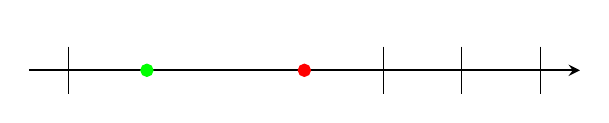
\begin{tikzpicture}[node distance=2cm,thick,every node/.style={transform shape}]
      \draw [thick,->,>=stealth] node [above,black] {} (-1,0) -- (6,0);
      \draw [thin] (-0.5,0.3) node [above,black] {$\xSS$} -- (-0.5,-0.3);
      \draw[mark=*,mark size=2pt,mark options={color=green}] plot coordinates {(0.5,0)};
      \draw[mark=*,mark size=2pt,mark options={color=red}] plot coordinates {(2.5,0)};
      \draw [thin]  (3.5,0.3) node [above,black] {$\xBL$} -- (3.5,-0.3);
      \draw [thin]  (4.5,0.3) node [above,black] {$\xSE$} -- (4.5,-0.3);
      \draw [thin]  (5.5,0.3) node [above,black] {$\xNC$} -- (5.5,-0.3);
    \end{tikzpicture}
    \caption{Dynamic entity has creation and deletion dates before the bulk load cut off. This entity is not serialized.}
    \label{fig:cond-1}
    \end{subfigure}
  %
    \begin{subfigure}{\linewidth}
    \centering
    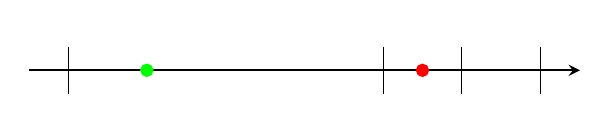
\begin{tikzpicture}[node distance=2cm,thick,every node/.style={transform shape}]
      \draw [thick,->,>=stealth] node [above,black] {} (-1,0) -- (6,0); % timeline
      \draw [thin] (-0.5,0.3) node [above,black] {$\xSS$} -- (-0.5,-0.3);
      \draw[mark=*,mark size=2pt,mark options={color=green}] plot coordinates {(0.5,0)};
      \draw [thin]  (3.5,0.3) node [above,black] {$\xBL$} -- (3.5,-0.3);
      \draw[mark=*,mark size=2pt,mark options={color=red}] plot coordinates {(4,0)};
      \draw [thin]  (4.5,0.3) node [above,black] {$\xSE$} -- (4.5,-0.3);
      \draw [thin]  (5.5,0.3) node [above,black] {$\xNC$} -- (5.5,-0.3);
    \end{tikzpicture}
        \caption{Dynamic entity has creation date before the bulk load cut off and a deletion date after the bulk load cut off, but before the simulation end. Such an entity is serialized into the bulk load component and spawns a delete operation.}
    \label{fig:cond-2}
  \end{subfigure}
  %
    \begin{subfigure}{\linewidth}
    \centering
    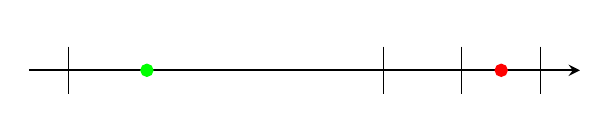
\begin{tikzpicture}[node distance=2cm,thick,every node/.style={transform shape}]
      \draw [thick,->,>=stealth] node [above,black] {} (-1,0) -- (6,0); % timeline
      \draw [thin] (-0.5,0.3) node [above,black] {$\xSS$} -- (-0.5,-0.3);
      \draw[mark=*,mark size=2pt,mark options={color=green}] plot coordinates {(0.5,0)};
      \draw [thin]  (3.5,0.3) node [above,black] {$\xBL$} -- (3.5,-0.3);
      \draw [thin]  (4.5,0.3) node [above,black] {$\xSE$} -- (4.5,-0.3);
      \draw[mark=*,mark size=2pt,mark options={color=red}] plot coordinates {(5,0)};
      \draw [thin]  (5.5,0.3) node [above,black] {$\xNC$} -- (5.5,-0.3);
    \end{tikzpicture}
        \caption{Dynamic entity has creation date before the bulk load cut off and a deletion date after the simulation end. Such an entity is in serialized only into the bulk load component.}
    \label{fig:cond-3}
  \end{subfigure}
    %
    \begin{subfigure}{\linewidth}
    \centering
    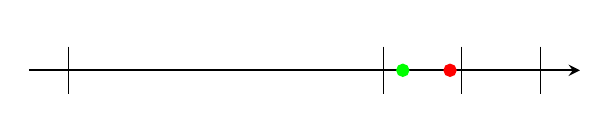
\begin{tikzpicture}[node distance=2cm,thick,every node/.style={transform shape}]
      \draw [thick,->,>=stealth] node [above,black] {} (-1,0) -- (6,0); % timeline
      \draw [thin] (-0.5,0.3) node [above,black] {$\xSS$} -- (-0.5,-0.3);
      \draw [thin]  (3.5,0.3) node [above,black] {$\xBL$} -- (3.5,-0.3);
      \draw[mark=*,mark size=2pt,mark options={color=green}] plot coordinates {(3.75,0)};
      \draw[mark=*,mark size=2pt,mark options={color=red}] plot coordinates {(4.35,0)};
      \draw [thin]  (4.5,0.3) node [above,black] {$\xSE$} -- (4.5,-0.3);
      \draw [thin]  (5.5,0.3) node [above,black] {$\xNC$} -- (5.5,-0.3);
    \end{tikzpicture}
    \caption{Dynamic entity has creation date after the bulk load cut off and a deletion date before the simulation end. Such an entity produces an insert operation and a delete operation.}
    \label{fig:cond-4}
  \end{subfigure}
    %
    \begin{subfigure}{\linewidth}
    \centering
    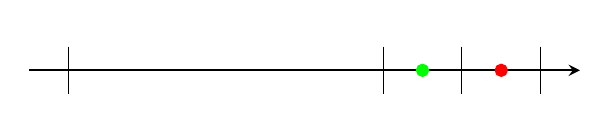
\begin{tikzpicture}[node distance=2cm,thick,every node/.style={transform shape}]
      \draw [thick,->,>=stealth] node [above,black] {} (-1,0) -- (6,0); % timeline
      \draw [thin] (-0.5,0.3) node [above,black] {$\xSS$} -- (-0.5,-0.3);
      \draw [thin]  (3.5,0.3) node [above,black] {$\xBL$} -- (3.5,-0.3);
      \draw[mark=*,mark size=2pt,mark options={color=green}] plot coordinates {(4,0)};
      \draw [thin]  (4.5,0.3) node [above,black] {$\xSE$} -- (4.5,-0.3);
      \draw[mark=*,mark size=2pt,mark options={color=red}] plot coordinates {(5,0)};
      \draw [thin]  (5.5,0.3) node [above,black] {$\xNC$} -- (5.5,-0.3);
    \end{tikzpicture}
        \caption{Dynamic entity has creation date after the bulk load cut off, but before the simulation end, and a deletion date after the simulation end. Such an entity produces only an insert operation.}
    \label{fig:cond-5}
  \end{subfigure}
  \caption{Possible dynamic entity \emph{creation} \textcolor{green}{$\bullet$} and \emph{deletion} \textcolor{red}{$\bullet$} dates with respect to simulation start, bulk load cut off, simulation end, and network collapse.}
  \label{fig:serialization-conds}
\end{figure}


\chapter{Workloads}\label{section:workloads}

\section{Query Description Format}
\label{sub:queries_structure}
Queries are described in natural language using a well-defined structure that consists of three sections:
\textit{description}, a concise textual description of the query;
\textit{parameters}, a list of input parameters and their types;
and \textit{results}, a list of expected results and their types.
The syntax used in \textit{parameters} and \textit{results} sections is as follows:

{\small
    \begin{itemize}
        \item \textbf{Entity}: entity type in the dataset.\\
            One word, possibly constructed by appending multiple words together, starting with uppercase character and following the camel case notation,
            \eg \texttt{TagClass} represents an entity of type ``TagClass''.
        \item \textbf{Relationship}: relationship type in the dataset.\\
            One word, possibly constructed by appending multiple words together, starting with lowercase character and following the camel case notation,
            and surrounded by arrow to communicate direction,
            \eg \texttt{-worksAt->} represents a directed relationship of type ``worksAt''.
        \item \textbf{Attribute}: attribute of an entity or relationship in the dataset.\\
            One word, possibly constructed by appending multiple words together, starting with lowercase character and following the camel case notation,
            and prefixed by a ``.'' to dereference the entity/relationship,
            \eg \texttt{Person.firstName} refers to ``firstName'' attribute on the ``Person'' entity,
            and \texttt{-studyAt->.classYear} refers to ``classYear'' attribute on the ``studyAt'' relationship.
        \item \textbf{Unordered Set}: an unordered collection of distinct elements.\\
            Surrounded by \{ and \} braces, with the element type between them,
            \eg \texttt{\{String\}} refers to a set of strings.
        \item \textbf{Ordered List}: an ordered collection where duplicate elements are allowed.\\
            Surrounded by [ and ] braces, with the element type between them,
            \eg \texttt{[String]} refers to a list of strings.
        \item \textbf{Ordered Tuple}: a fixed length, fixed order list of elements, where elements at each position of the tuple have predefined, possibly different, types. \\
            Surrounded by < and > braces, with the element types between them in a specific order
            \eg \texttt{<String, Boolean>} refers to a 2-tuple containing a string value in the first element and a boolean value in the second,
            and \texttt{[<String, Boolean>]} is an ordered list of those 2-tuples.
    \end{itemize}
}
\chapter{Interactive Workload}\label{section:workload}

\section{Query Specifications}

\subsection{Complex Reads Query Descriptions}

\input{query-cards/interactive-complex-read-01}
\input{query-cards/interactive-complex-read-02}
\input{query-cards/interactive-complex-read-03}
\input{query-cards/interactive-complex-read-04}
\input{query-cards/interactive-complex-read-05}
\input{query-cards/interactive-complex-read-06}
\input{query-cards/interactive-complex-read-07}
\input{query-cards/interactive-complex-read-08}
\input{query-cards/interactive-complex-read-09}
\input{query-cards/interactive-complex-read-10}
\input{query-cards/interactive-complex-read-11}
\input{query-cards/interactive-complex-read-12}
\input{query-cards/interactive-complex-read-13}
\input{query-cards/interactive-complex-read-14}

\subsection{Short Reads Query Descriptions}

\todo{These could also be reworked as query cards.}
\input{interactive-short-reads}

%\input{query-cards/interactive-short-read-01}

\subsection{Update Query Descriptions}

\todo{Maybe introduce YAML specification for these as well?}
\input{interactive-update}

\section{Substitution Parameters}

\input{interactive-parameters}

\section{Load Definition}


\input{interactive-workload}

\subsection{Business Intelligence Workload}
\subsubsection{Choke Points}

\subsubsection{Business Intelligence Queries}

{\small
    \begin{enumerate}
      \item Posting summary 
            \begin{itemize}
                \item \textbf{Description:}
                  Given a date, find all Messages (Posts and Comments) created before than that date.
                  Group them by a three level grouping.

                  \begin{itemize}
                    \item First: by their year of creation.
                    \item Second: for each year, group them into Posts and Comments.
                    \item Third: for each year-type (Post or Comment) group, split it into four groups based on the
                              length of their content: 
                              \begin{itemize}
                                \item if length is less than 40, it is 'short'; 
                                \item else, if length is less than 80, it is 'one liner';
                                \item else, if length is less than 160, it is 'tweet';
                                \item otherwise, it is 'long'
                              \end{itemize}
                  \end{itemize}

                \item \textbf{Parameters:} \\
                    \begin{tabular}{ll}
                      date 										& DateTime \\
                    \end{tabular}
                \item \textbf{Results:} \\
                  For every third-level group, return the the following aggregates:
                    \begin{tabular}{lll}
                      year 					& 32-bit Integer & \\
                      Message.type	& String & \parbox[t]{20cm}{// "Post" or "Comment"  \strut} \\
                      Message.length & 32-bit Integer & \\
                      category & 32-bit Integer & \parbox[t]{20cm}{// 0 (short), 1 (one-liner), 2 (tweet), 3 (long) \strut}  \\
                      count & 32-bit Integer &  \parbox[t]{20cm}{// The number of messages in this group  \strut} \\
                      average & 32-bit Integer &  \parbox[t]{20cm}{// The average Message length \strut} \\
                      sum & 32-bit Integer &  \parbox[t]{20cm}{// The sum of the Messages lengths \strut} \\
                      percentage & 32-bit Floating Point &  \parbox[t]{20cm}{// The percentage of Messages in this group
                        out of the total number \par of Messages created before the given date  \strut} \\
                      \end{tabular}
                    Sort the results first by Year (descending), then by the Message.type (Post 1st, or Comment 2nd) and
                    finally by the category (ascending)
                    \end{itemize}

      \item Top Tags from Country, age, gender and time 
            \begin{itemize}
                \item \textbf{Description:}
                  Select all Messages created between date1 and date2 (both included) by Persons located in any country
                  of a provided list of countries Select the creators (Persons) and the Tags of these Messages .  Split
                  these persons, tags and Messages into a five level grouping:
                  \begin{itemize}
                    \item First by the name of the country of the Person
                    \item  Second, by the month when the Message was created
                    \item Third, by the gender of the person
                    \item      Four, by the age group of the Person, which is defined as:
                      \begin{itemize}
                        \item The difference in years between the Person's birthday and the end of
                          simulation ('2013-01-01'), divided by 5, rounded down.
                      \end{itemize}
                    \item  Fifth, by the name of the tag attached to the Message
                  \end{itemize}
                \item \textbf{Parameters:} \\
                    \begin{tabular}{ll}
                      date1 & Date \\
                      date2 & Date \\
                      list of country names & \{String\} \\
                      endDate & Date \\
                    \end{tabular}
                \item \textbf{Results:} \\
                  For each of the fifth-level groups return: 
                    \begin{tabular}{lll}
                      Country.name & String & \\
                      month & 32-bit Integer & \\
                      gender & String & \parbox[t]{20cm}{// "Male" or "Female" \strut}\\
                      age group & 32-bit Integer & \\
                      Tag.name & String & \\
                      count & 32-bit Integer & \parbox[t]{20cm}{// The count of Messages falling in this group \strut}
                    \end{tabular}
                    Return top 100 groups where number of Messages is bigger than 100. Sort the groups by the count
                    (descending), Tag name (ascending), age group (ascending), gender (ascending), month
                    (ascending) and country name (ascending).
                    \end{itemize}
      \item Tag Evolution 
            \begin{itemize}
                \item \textbf{Description:}
                  Given two date intervals (left-closed, right-open), for each of these intervals find all Tags that
                  were used in Messages. For each interval, count the number of Messages containing each Tag.

                \item \textbf{Parameters:} \\
                    \begin{tabular}{ll}
                      dateStart1 & Date \\
                      dateEnd1 & Date \\
                      dateStart2 & Date \\
                      dateEnd2 & Date \\
                    \end{tabular}
                \item \textbf{Results:} \\
                  For each of the tags:
                    \begin{tabular}{lll}
                      Tag.name & String & \\
                      countInterval1 & 32-bit Integer & \parbox[t]{20cm}{// The number of occurrences of this Tag during
                        interval 1  \strut} \\
                      countInterval2 & 32-bit Integer & \parbox[t]{20cm}{// The number of occurrences of this Tag during
                        interval 2 \strut}\\
                      diff & 32-bit Integer & \parbox[t]{20cm}{ // The absolute difference countInterval1 and
                        countInterval2 \strut} \\
                    \end{tabular}
                    Return top-100 results sorted by the difference (descending) and then the tag name (ascending)
                    \end{itemize}

      \item Popular topics in a Country 
            \begin{itemize}
                \item \textbf{Description:}
                  Given a tagCalss and a Country, find all the Forums created in the given Country, containing at least
                  one Posts with Tags belonging directly to the given tagClass.
                  The location of a Forum is identified by the location of the Forum’s moderator.
                \item \textbf{Parameters:} \\
                    \begin{tabular}{ll}
                      TagClass.name & String \\
                      Country.name & String \\
                    \end{tabular}
                \item \textbf{Results:} \\
                  For each Forum:
                    \begin{tabular}{lll}
                      Forum.id  & ID & \\
                      Forum.title & String & \\
                      Forum.creationDate & DateTime & \\
                      Forum-hasModerator->Person.id & \{ ID \} & \\
                      count & 32-bit Integer &  \parbox[t]{20cm}{ // The number of Posts in the Forum with at least \par one Tag belonging to
                        the TagClass \strut} 
                    \end{tabular}
                    Return top-20 results sorted by count (descending) and Forum.id (ascending)
                    \end{itemize}

      \item Top posters in a Country 
            \begin{itemize}
                \item \textbf{Description:}
                  Find the most popular Forums for a given Country, where the popularity of a Forum is measured by the
                  number of members that Forum has from the given Country.  If multiple forums have the same member
                  count, use forum ID as tie breaker for popularity, where lower ID is more popular.  For each person
                  that is a member or moderator of any of the 100 most popular Forums, count the number of Posts they
                  made in any of those (most popular) Forums.

                  Group persons by:
                  \begin{itemize}
                      \item First, id
                      \item Second, first name
                      \item Third, last name
                      \item Fourth, creation date
                  \end{itemize}
                \item \textbf{Parameters:} \\
                    \begin{tabular}{ll}
                      Country.name & String \\ 
                    \end{tabular}
                \item \textbf{Results:} \\
                   For each group:
                    \begin{tabular}{lll}
                      Person.id & ID & \\
                      Person.firstName & String & \\
                      Person.lastName & String & \\
                      Person.creationDate & DateTime & \\
                      count & 32-bit Integer & \parbox[t]{20cm}{ // Number of Posts created by that Person \par in the top-100
                        most popular Forums\strut}  \\
                    \end{tabular}
                    Return top 100 Persons, sorted by count (descending) and by Person.Id (ascending).
                    \end{itemize}

      \item Most active posters on a given topic 
            \begin{itemize}
                \item \textbf{Description:}
                  Retrieve Persons who have created a Message with given Tag.  For each Person, compute a score as
                  follows: (the number of Messages they created that have given Tag) PLUS (2 x number of replies to
                  those Messages) PLUS (10 x number of Likes on those Messages).
                \item \textbf{Parameters:} \\
                    \begin{tabular}{ll}
                      Tag.name & 32-bit Integer 
                    \end{tabular}
                \item \textbf{Results:} \\
                  For each Person:
                    \begin{tabular}{lll}
                      Person.id & ID & \\
                      replyCount & 32-bit Integer & \parbox[t]{20cm}{ //The number of replies to Messages with
                        the \par given Tag created by the Person \strut}  \\
                      likeCount & 32-bit Integer & \parbox[t]{20cm}{ //The number of likes to Messages with
                        the \par given Tag created by the Person \strut}  \\ 
                      messageCount & 32-bit Integer & \parbox[t]{20cm}{ //The number of Messages with
                        the \par given Tag created by the Person \strut}  \\
                      score & 32-bit Integer & \\
                    \end{tabular}
                    Return the top-100 Persons, sorted by score (descending) and Person.id (ascending)
                    \end{itemize}

      \item Most authorative Person on a given topic 
            \begin{itemize}
                \item \textbf{Description:}
                  Given a Tag, find all Persons that ever created a Message with the given Tag.
                  For each of these Persons compute their "authority score".
                  The "authority score" for a given Person is defined as the sum of "popularity scores" of the Persons
                  that liked any of that Person's Messages with the given Tag.
                  A Person's "popularity score" is defined as the total number of likes on all of their Messages.
                \item \textbf{Parameters:} \\
                    \begin{tabular}{ll}
                      Tag.name & String \\
                    \end{tabular}
                \item \textbf{Results:} \\

                  For each Person:

                    \begin{tabular}{lll}
                      Person.Id & ID & \\
                      authorityScore & 32-bit Integer & \\
                    \end{tabular}

                    Return the top 100 Persons sorted the authorityScore (descending) and Person.Id (ascending).
                    \end{itemize}

      \item Related Topics 
            \begin{itemize}
                \item \textbf{Description:}
                  Find all Messages that have a given Tag.    
                  Find the Tags attached to replies of these Messages, but only those replies that do not have the given
                  Tag. Group the Tags by name, and get the count of replies in each group.
                \item \textbf{Parameters:} \\
                    \begin{tabular}{ll}
                      Tag.name & String \\
                    \end{tabular}
                \item \textbf{Results:} \\
                  For each group:
                    \begin{tabular}{lll}
                      Tag.name & String & \\
                      count & 32-bit Integer & \parbox[t]{20cm}{ // The count of replies with the Tag \strut} \\
                    \end{tabular}
                    Return the top-100 Tags, sorted by count (descending) and by Tag.name (ascending).
                    \end{itemize}

      \item Forum with related Tags 
            \begin{itemize}
                \item \textbf{Description:}
                  Given two tagClasses, find those forums that contain Posts with Tags belonging tagClass1 and contain
                  Posts with Tags belonging to tagCalss2 (not transitive). Consider the forums with a number of members
                  greater than a given threshold.
                  For every such forum, count the number of Posts  that have a Tag from tagclass t1 (count1), and the
                  number of posts that have a tag  from the tagclass2. 
                \item \textbf{Parameters:} \\
                    \begin{tabular}{ll}
                      TagClass1.name & String \\ 
                      TagClass2.name & String \\ 
                      threshold & 32-bit Integer \\
                    \end{tabular}
                \item \textbf{Results:} \\
                  For each Forum:
                    \begin{tabular}{lll}
                      Forum.id & ID & \\
                      count1 & 32-bit Integer & \parbox[t]{20cm}{ // The count of Posts with at least one Tag belonging
                        to TagClass1 \strut} \\
                      count2 & 32-bit Integer & \parbox[t]{20cm}{ // The count of Posts with at least one Tag belonging
                        to TagClass2 \strut} \\
                    \end{tabular}
                    \end{itemize}

      \item Central Person for a topic 
            \begin{itemize}
                \item \textbf{Description:}
                  Given a Tag, find all Persons that are either interested on the Tag, or have written a Post with the
                  given Tag. For each Person, compute the score as the sum of the following two aspects:

                  \begin{itemize}
                    \item 100, if the Person has this tag as their interest, or 0 otherwise
                    \item number of posts by this person with the given tag
                  \end{itemize}

                \item \textbf{Parameters:} \\
                    \begin{tabular}{ll}
                      Tag.name & String \\
                    \end{tabular}
                \item \textbf{Results:} \\
                  For each Person:

                    \begin{tabular}{lll}
                      Person.Id & ID & \\
                      score & 32-bit Integer & \\
                      friendsScore & 32-bit Integer & \parbox[t]{20cm}{ // The sum of the score of the Person's friends\strut} \\
                    \end{tabular}

                    Return the top-100 Persons, sorted the sum of score and friendsScore (descending), and  Person.id
                    (ascending) 
                \end{itemize}

      \item Tag Evolution 
            \begin{itemize}
                \item \textbf{Description:}
                \item \textbf{Parameters:} \\
                    \begin{tabular}{ll}
                    \end{tabular}
                \item \textbf{Results:} \\
                    \begin{tabular}{lll}
                    \end{tabular}
                    \end{itemize}
\end{enumerate}
}


%\section{Performance metrics}\label{section:metrics}
\alert{ TODO} 
%\alert{ TODO - Renzo \\
%Here we need to describe the different metrics used to evaluate the performance
%of the systems.
%}
%
%\subsection{Response Time}
%
%Response Time (RT) is defined by RT = eT - sT where:
%\begin{itemize}
%    \item sT = time measured before the first byte of input data of the Transaction is sent by the Driver to the SUT; 
%    \item eT = time measured after the last byte of output data from the Transaction is received by the Driver from the SUT.
%\end{itemize}
%The resolution of the time stamps used for measuring Response Time is of at least \alert{XX} seconds.
%
%\subsection{Throughput}
%
%The throughput is measured as ''Operations per second at scale'' (i.e.  opsSI@100).
%The metric is calculated for a run that satisfies the minimum length and per
%query minimum execution count and query mix criteria.
%\alert{Describe here the criteria}
%Each completed operation counts as one operation. The metric is the count of successful operations
%divided by elapsed time in seconds.
%
%\subsection{Interactive Workload Metric}
%
%\alert{Need to elaborate on this. The current description in confluence is incomplete. Is this needed?}
%
%
%\subsection{Price/Performance Metric}
%\alert{We need to include the definition of a price/performance metric.}




%\section{Execution rules}\label{section:rules}

%\subsection{Execution Steps}
%\alert{Some items have to be reviewed}
%A benchmark execution is divided into the following steps:
%\begin{itemize}
%    \item \textbf{Data Preparation.} This includes running the data generator, placing
%        the generated files in a staging area, configuring storage, setting up
%        the SUT configuration and preparing any data partitions in the SUT.
%        This may include pre-allocating database space but may not include
%        loading any data or defining any schema having to do with the
%        benchmark.
%    \item \textbf{Bulk Load.} This includes defining the database schema, if any,
%        loading the initial database population, making this durably stored,
%        gathering any optimizer statistics,.   The bulk load time is reported
%        and is equal to the amount of elapsed wall clock time between starting
%        the schema definition and receiving the confirmation message of the end
%        of statistics gathering.
%    \item \textbf{Benchmark Run.} The run begins after the bulk load or after another
%        benchmark run.  If the run does not directly follow the bulk load, it
%        must start at a point in the update stream that has not previously been
%        played into the database.  In other words, a run may only include
%        update events whose timestamp is later than the latest post creation
%        date in the database prior to start of run.  The run starts when the
%        first of the test drivers sends its first message to the SUT.  If the
%        SUT is in-process with the driver the window starts when the driver
%        starts.
%    \item \textbf{Measurement Window.} The measurement window is the timed portion of
%        the benchmark run. It may begin at any time during the run.  The
%        activity during the measurement window must meet the criteria described in
%        \alert{Section XX}. The measurement window is terminated at
%        the discretion of the test sponsor at any time when the Minimum
%        Measurement Window criteria are met. All the processes constituting
%        the SUT are to be killed at the end of the window or alternatively all
%        the hardware components of the SUT are to be powered off.
%    \item \textbf{Recovery Test.} The SUT is to be restarted after the measurement
%        window and the auditor will verify that the SUT contains the entirety
%        of the last update recorded by the test driver(s) as successfully
%        committed.
%\end{itemize}
%
%\subsection{Rules for the Data Schema}
%
%\ldbcsnb may be implemented with different data models, \eg relational, RDF and
%different graph data models.  The reference schema is provided as RDFS and SQL.
%The data generator produces TTL syntax for RDF and comma separated values for
%other data models. A single attribute has a single data type. The following
%requirements apply:
%
%\begin{itemize}
%    \item \textbf{Identifier:} This is an integer value foreign key or a URI in
%        RDF.  If this is an integer column, the implementation data type should
%        support at least $2^{55}$ distinct values
%    \item \textbf{Datetime:} Should support a date range from 0000 to 9999 in
%        the year field, with a resolution of no less than one second.
%    \item \textbf{String:} A string column for names may have a variable length
%        and may have a declared maximum length, \eg 40 characters.
%    \item \textbf{Long String:} For example a post content may be a long string
%        that is often short in the data but may not declare a maximum length
%        and must support data sizes of up to 1MB \alert{Current generator max post length is set to 2000 characters}..
%\end{itemize}
%
%A single attribute in the reference schema may not be divided into multiple
%attributes in the target schema.
%
%
%A schema on the DBMS is optional.  An RDF implementation for example may work
%without one.  An RDF implementation is allowed to load the RDF reference schema
%and to take advantage of the data type and cardinality statements therein.
%
%
%A relational or graph schema may specify system specific options affecting
%storage layout.  These may for example specify vertical partitioning.  Vertical
%partitioning means anything from a column store layout with per-column
%allocated storage space to use of explicit column groups.  Any mix of row or
%column-wise storage structures is allowed as long as this is declaratively
%specified data structure by data structure.  Data structure here means for
%example table or index.
%
%
%Covering indices and clustered indices are allowed.
%If these are defined, then all replications of data implied by these must be
%maintained statement by statement, \ie each auxiliary data structure must be
%consistent with any other data structures of the table after each data
%manipulation operation.
%
%
%A covering index is an index which materializes a
%specific order of a specific subset or possibly all columns of a table.  A
%clustered index is an index which materializes all columns of a table in a
%specific order, which order may or may not be that of the primary key of the
%table. A clustered or covering index may be the primary or only representation
%of a table.
%
%
%Any subset of the columns on a covering or clustered index may be
%used for ordering the data.  A hash based index or a combination of a hash
%based and tree based index are all allowed, in row or column-wise or hybrid
%forms.
%
%
%\subsection{Rules for Implementing the Workload}
%\subsubsection{Queries' Implementation}
%
%The queries and updates may be implemented in a declarative query language or
%as procedural code using an API.  If a declarative query language is used, \eg
%SPARQL or SQL, then explicit query plans are prohibited in all the read-only
%queries. The update transactions may still consist of multiple statements,
%effectively amounting to explicit plans.
%
%
%Explicit query plans include but \alert{are not limited to (this is too ambiguous and dangerous)}:
%\begin{itemize}
%    \item Directives or hints specifying a join order or join type
%    \item Directives or hints specifying an access path, \eg which index to use
%    \item Directive or hints specifying an expected cardinality, selectivity,
%        fanout or any other information that pertains to the expected number or
%        results or cost of all or part of the query.
%\end{itemize}
%
%\subsubsection{Auxiliary Data Structures and Pre-computation}
%Auxiliary data structures and pre-computations are allowed.  A pre-computation
%may be implemented as client side logic in the test driver, as stored
%procedures or as triggers.  In all cases the operations, whether one or many,
%must constitute a single transaction.  A SPARQL protocol operation consisting
%of multiple statements may be a valid implementation of the if the SUT executes
%the statements as a single transaction. Other pre-computation of query results
%is explicitly prohibited.
%
%\subsubsection{ACID Compliance}
%
%The interactive workload requires full ACID support from the SUT.
%\begin{itemize}
%    \item \textbf{Atomicity.} All the updates in a transaction must either take
%        place or be all cancelled.
%    \item \textbf{Consistency.} If a database object, \eg table, has auxiliary
%        data structures, \eg indices, the content of these must be consistent
%        after the commit or rollback of a transaction.   If multiple client
%        application threads share one transaction context, these may
%        transiently see inconsistent states, \eg there may be a time when an
%       insert of a row is reflected in one index of a table but not in
%        another.
%    \item \textbf{Isolation.} If a transaction reads the database with intent
%        to update, the DBMS must guarantee that repeating the same read within
%        the same transaction will return the same data.  This also means that
%        no more and no less data rows must be returned.  In other words, this
%        corresponds to snapshot or to serializable isolation.  This level of
%        isolation is applied for the operations where the transaction mix so
%        specifies.  If the database is accessed without transaction context or
%        without intent too update, then the DBMS should provide read committed
%        semantics, \eg repeating the same read may produce different results
%        but these results may never include effects of pending uncommitted
%        transactions.
%    \item \textbf{Durability.} The effects of a transaction must be made
%        durable against instantaneous failure before the SUT confirms the
%        successful commit of a transaction to the application. For systems
%        using a transaction log, this implies syncing the durable media of the
%        transaction log before confirming success to the application.  This
%        will typically entail group commit where transactions that fall in the
%        same short window are logged together and the logging device will
%        typically be an SSD or battery backed RAM on a storage controller.  For
%        systems using replication for durability, this will entail receipt of a
%        confirmation message from the replicating party before confirming
%        successful commit to the application.
%\end{itemize}
%
%\subsection{Rules for Running the Test Driver}
%
%A qualifying run must use the \ldbcsnb test driver provided. The test driver
%implements the workload described in \alert{Section XX}.
%The test driver may be modified by the test sponsor for purposes of
%interfacing to the SUT. The parameter generation and result recording and
%workload scheduling parts of the test driver cannot be changed.  The
%auditor needs to have access to the test driver source code used for producing
%the driver used in the reported run.
%
%\alert{ Check whether this is out of date or not}
%
%The test driver is scale-out capable.  Many
%instances of the test driver may be used in a test run.   The number and
%configuration of the test drivers must be disclosed, along with hardware
%details of the platform running the driver(s), together with details of the
%network interface connecting the drivers too the SUT.  The SUT hardware may
%also be used for hosting the driver(s), at the discretion of the test sponsor.
%
%
%A separate test summary tool provided with the test driver analyzes the test
%driver log(s) after a measurement window is completed.  The tool produces for
%each of the distinct queries and transactions the following summary:
%\begin{itemize}
%    \item Count of executions
%    \item Minimum/average/90th percentile/maximum execution time.
%    \item Start and end date of the window in real time and in simulation time.
%    \item Metric in operations per second at scale. (ops) (throughout rating)
%    \item Number of test drivers
%    \item Number of database sessions (threads) per test driver
%\end{itemize}
%
%
%\subsection{Rules for Scaling}
%\ldbcsnb provides predefined scale factors, as described in \alert{Section XX}.
%The validation scale factor is 1.  Official \ldbcsnb results may be published at
%any of the provided scale factors.
%
%
%\subsection{Rules for Checkpointing}
%A checkpoint is defined as the operation which causes data persisted in a
%transaction log to become durable outside of the transaction log. In specific,
%this means that a SUT restart after instantaneous failure following the
%completion of the checkpoint may not have recourse to transaction log entries
%written before the end of the checkpoint.
%
%
%A checkpoint typically involves a
%synchronization barrier at which all data committed prior too the moment is
%required to be in durable storage that does not depend on the transaction log.
%
%
%Not all DBMSs use a checkpointing mechanism for durability. For example a
%system may rely on redundant storage of data for durability guarantees against
%instantaneous failure of a single server.
%
%
%The measurement window may contain a
%checkpoint. If the measurement window does not contain one, then the restart
%test will involve redoing all the updates in the window as part of the recovery
%test.

%\section{Full disclosure}\label{section:disclosure}
\alert{ TODO }
%\alert{ TODO - Peter, Larri and Orri \\
%Here we have to describe what needs to be disclosed to have a valid benchmark report.
%}

%\chapter{Auditing Policies}
\label{sec:auditing}

\emph{This chapter contains the auditing policies for the LDBC Social Network Benchmark. The initial draft of the auiting policies were published in the EU project deliverable D6.3.3 ``LDBC Benchmark Auditing Policies''.}

%%%%%%%%%%%%%%%%%%%%%%%%%%%%%%%%%%%%%%%%%%%%%%%%%%%%%%%%%%%%%%%%%%%%%%%%%%%%%%
%%%%%%%%%%%%%%%%%%%%%%%%%%%%%%%%%%%%%%%%%%%%%%%%%%%%%%%%%%%%%%%%%%%%%%%%%%%%%%
%%%%%%%%%%%%%%%%%%%%%%%%%%%%%%%%%%%%%%%%%%%%%%%%%%%%%%%%%%%%%%%%%%%%%%%%%%%%%%

This chapter is divided in the following parts:
\begin{itemize}
    \item Motivation of benchmark result auditing
    \item General discussion of auditable aspects of benchmarks
    \item Specific checklists and running rules for the Social Network Benchmark's workloads (Interactive, Business Intelligence)
\end{itemize}

Many definitions and general considerations are shared between the benchmarks, hence it is justified to present the principles first and to refer to these in the context of the benchmark specific rules.

The auditing process, including the auditor certification exams, the possibility of challenging audited results, \etc, are defined in the LDBC Byelaws~\cite{ldbc_byelaws}. Please refer to the latest Byelaws document when conducting audits.

%%%%%%%%%%%%%%%%%%%%%%%%%%%%%%%%%%%%%%%%%%%%%%%%%%%%%%%%%%%%%%%%%%%%%%%%%%%%%%
%%%%%%%%%%%%%%%%%%%%%%%%%%%%%%%%%%%%%%%%%%%%%%%%%%%%%%%%%%%%%%%%%%%%%%%%%%%%%%
%%%%%%%%%%%%%%%%%%%%%%%%%%%%%%%%%%%%%%%%%%%%%%%%%%%%%%%%%%%%%%%%%%%%%%%%%%%%%%

\section{Rationale and General Principles}

%%%%%%%%%%%%%%%%%%%%%%%%%%%%%%%%%%%%%%%%%%%%%%%%%%%%%%%%%%%%%%%%%%%%%%%%%%%%%%
%%%%%%%%%%%%%%%%%%%%%%%%%%%%%%%%%%%%%%%%%%%%%%%%%%%%%%%%%%%%%%%%%%%%%%%%%%%%%%
%%%%%%%%%%%%%%%%%%%%%%%%%%%%%%%%%%%%%%%%%%%%%%%%%%%%%%%%%%%%%%%%%%%%%%%%%%%%%%

The purpose of benchmark auditing is to improve the \emph{credibility} and \emph{reproducibility} of benchmark claims by involving a set of detailed execution rules and third party verification of compliance with these.

Rules may exist separately of auditing but auditing is not meaningful unless the rules are adequately precise.
Aspects like auditor training and qualification cannot be addressed separately from a discussion of the matters the
auditor is supposed to verify. Thus the credibility of the entire process hinges on clear and shared understanding
of what a benchmark is expected to demonstrate and on the auditor being capable of understanding the process
and of verifying that the benchmark execution is fair and does not abuse the rules or pervert the objectives of
the benchmark.

Due to the open-ended nature of technology and the agenda of furthering innovation via measurement, it is
not feasible or desirable to over-specify the limits of benchmark implementation. Hence there will always remain
judgement calls for borderline cases. In this respect auditing and the LDBC are not separate. It is expected that
issues of compliance as well as of maintenance of rules will come before the LDBC as benchmark claims are
made.

%%%%%%%%%%%%%%%%%%%%%%%%%%%%%%%%%%%%%%%%%%%%%%%%%%%%%%%%%%%%%%%%%%%%%%%%%%%%%%
%%%%%%%%%%%%%%%%%%%%%%%%%%%%%%%%%%%%%%%%%%%%%%%%%%%%%%%%%%%%%%%%%%%%%%%%%%%%%%
%%%%%%%%%%%%%%%%%%%%%%%%%%%%%%%%%%%%%%%%%%%%%%%%%%%%%%%%%%%%%%%%%%%%%%%%%%%%%%

\section{Auditing Rules Overview}


\subsection{Auditor Training, Certification, and Selection}
\subsubsection{Auditor Training}
Auditor training consists of familiarisation with the benchmark and existing implementations thereof. This involves the auditor candidate running the reference implementations of the benchmark in order to see what is normal behaviour and practice in the workload. The training and practice may involve communication with the benchmark task force for clarifying intent and details of the benchmark rules. This produces feedback for the task force for further specification of the rules.

\subsubsection{Auditor Certification}
The auditor certification and qualification is done in the form of an examination administered by the task force responsible for the benchmark being audited. The examination may be carried out by teleconference. The task force will subsequently vote on accepting each auditor, by simple majority. An auditor is certified for a particular benchmark by the task force maintaining the benchmark in question.

\subsubsection{Auditor Selection}
In the default auditor selection, the task force responsible for the benchmark being audited appoints a third party, impartial auditor. The task force may in special cases appoint itself as auditor of a particular result. This is not, however, the preferred course of action but may be done if no suitable third party auditor is available


\subsection{Auditing Process Stages}
\subsubsection{Getting Ready for a Benchmark Audit}
A benchmark result can be audited if it is a \emph{complete implementation} of an LDBC benchmark workload. This includes implementing all operations (reads and updates) correctly, using official data sets, using the official LDBC driver (if available), and complying with the auditing rules of the workload (\eg workloads may have different rules regarding query languages, the allowance of materialized views, \etc).
Workloads may specify further requirements such as ACID-compliance (checked using the LDBC ACID test suite).

\subsubsection{Performing a Benchmark Audit}
A benchmark result is to be audited by an LDBC appointed auditor or the LDBC task force managing the benchmark. An LDBC audit may be performed by remote login and does not require the auditor's physical presence on site. The test sponsor shall grant the auditor any access necessary for validating the benchmark run. This will typically include administrator access to the SUT hardware.

\subsubsection{Benchmark-Specific Checklist}
Each benchmark specifies a checklist to be verified by the auditor. The benchmark run shall be performed by the auditor. The auditor shall take copies of relevant configuration files and test results for future checking and insertion into the full disclosure report.

\subsubsection{Producing the FDR}
The FDR is produced by the auditor or auditors, with any required input from the test sponsor. Each non-default configuration parameter needs to be included in the FDR and justification needs to be provided why the given parameter was changed.
The auditor produces an attestation letter that verifies authenticity of the presented results. This letter is to be included into the FDR as an addendum. The attestation letter has no specific format requirements but shall state that the auditor has established compliance with a specified version of the benchmark specification.

\subsubsection{Publishing the FDR}
The FDR and any benchmark specific summaries thereof shall be published on the LDBC website, \url{https://ldbcouncil.org/}.

\subsection{Challenge Procedure}

A benchmark result may be \emph{challenged} for non-compliance with LDBC rules. The benchmark task force responsible for maintenance of the benchmark will rule on matters of compliance. A result found to be non-compliant will be withdrawn from the list of official LDBC benchmark results.

%%%%%%%%%%%%%%%%%%%%%%%%%%%%%%%%%%%%%%%%%%%%%%%%%%%%%%%%%%%%%%%%%%%%%%%%%%%%%%
%%%%%%%%%%%%%%%%%%%%%%%%%%%%%%%%%%%%%%%%%%%%%%%%%%%%%%%%%%%%%%%%%%%%%%%%%%%%%%
%%%%%%%%%%%%%%%%%%%%%%%%%%%%%%%%%%%%%%%%%%%%%%%%%%%%%%%%%%%%%%%%%%%%%%%%%%%%%%

\section{Auditable Properties of Systems and Benchmark Implementations}

%%%%%%%%%%%%%%%%%%%%%%%%%%%%%%%%%%%%%%%%%%%%%%%%%%%%%%%%%%%%%%%%%%%%%%%%%%%%%%
%%%%%%%%%%%%%%%%%%%%%%%%%%%%%%%%%%%%%%%%%%%%%%%%%%%%%%%%%%%%%%%%%%%%%%%%%%%%%%
%%%%%%%%%%%%%%%%%%%%%%%%%%%%%%%%%%%%%%%%%%%%%%%%%%%%%%%%%%%%%%%%%%%%%%%%%%%%%%

\subsection{Validation of Query Results}
\label{sec:validation}
A benchmark should be published with a deterministically reproducible validation data set. Validation queries applied to the validation data set will deterministically produce a set of correct answers. This is used in the first stage of benchmark run to test for the correctness of an SUT or benchmark implementation. This validation stage is not timed.

\paragraph{Inputs for validation}
The validation takes the form of a set of data generator parameters, a set of test queries that at least include one instance of each of the workload query templates and the expected results.

\paragraph{Approximate results and error margin}
In certain cases the results may be approximate. This may happen in cases of non-unique result ordering keys, imprecise numeric data types, random behaviours in certain graph analytics algorithms etc. Therefore, a validation set shall specify the degree of allowable error: For example, for counts, the value must be exact, for sums, averages and the like, at least 8 significant digits are needed, for statistical measures like graph centralities, the result must be within 1\% of the reference result. Each benchmark shall specify its expectation in an unambiguously verifiable manner.

\subsection{ACID Compliance}
\label{sec:acid-compliance}

As part of the auditing process for the Interactive workload and for certain systems in the BI workload, the auditors ascertain that the SUT satisfies the ACID properties,
\ie it provides atomic transactions, complies with its claimed isolation level, and ensures durability in case of failures.
This section outlines transactional behaviours of SUTs which are checked in the course of auditing an SUT in a given benchmark.

A benchmark specifies transactional semantics that may be required for different parts of the workload. The requirements will typically be different for initial bulk load of data and for the workload itself. Different sections of the workload may further be subject to different transactionality requirements.

No finite series of tests can prove that the ACID properties are fully supported. Passing the specified tests is a necessary, but not sufficient, condition for meeting the ACID requirements. However, for fairness of reporting, only the tests specified here are required and must appear in the FDR for a benchmark. (This is taken exactly from the \mbox{TPC-C} specification~\cite{tpcc}.)

The properties for ACID compliance are defined as follows:

\paragraph{Atomicity}
Either all of the effects of the transaction are in effect after the transaction or none of the effects
is in effect. This is by definition only verifiable after a transaction has finished.

\paragraph{Consistency}
ADS such as secondary indices will be consistent among themselves as well as with the table or other PDS, if any. Such a consistency (compliance to all constraints, if these are declared in the schema, \eg primary key constraint, foreign key constraints and cardinality constraints) may be verified
after the commit or rollback of a transaction. If a single thread of control runs within a transaction, then
subsequent operations are expected to see consistent state across all data indices pertaining to a table
or similar object. Multiple threads which may share a transaction context are not required to observe a
consistent state at all times during the execution of the transaction. Consistency will however always be
verifiable after the commit or rollback of any transaction, regardless of the number of threads that have
either implicitly or explicitly participated in the transaction. Any intra-transaction parallelism introduced
by the SUT will preserve transactional semantics statement-by-statement. If explicit, application created
sessions share a transaction context, then this definition of consistency does not hold: for example, if
two threads insert into the same table at the same time in the same transaction context, these may or may
not see a consistent image of (E)ADS for the parts affected by the other thread. All things will be
consistent after the commit or rollback, however, regardless of the number of threads, implicit or explicit
that have participated in the transaction.

\paragraph{Isolation}
Isolation is defined as the set of phenomena that may (or may not) be observed by operations running within a single transaction context. The levels of isolation are defined as follows:

\begin{description}
\item[Read uncommitted] No guarantees apply.
\item[Read committed] A transaction will never read a value that has at no point in time been part of a
    committed state.
\item[Repeatable read] If a transaction reads a value several times during its execution, then it will see
    the original state with its own modifications so far applied to it. If the transaction itself consists of
    multiple reading and updating threads then the ambiguities that may arise are beyond the scope of transaction isolation.
\item[Serializable] The transactions see values that correspond to a fully serial execution of
    all client transactions. This is like repeatable read except that if the transaction reads something, and
    repeats the read, it is guaranteed that no new values will appear for the same search condition on a
    subsequent read in the same transaction context. For example, a row that was seen not to exist when
    first checked will not be seen by a subsequent read. Likewise, counts of items will not be seen to
    change.
\end{description}

\paragraph{Durability}
Durability means that once the SUT has confirmed a successful commit, the committed state
will survive any instantaneous failure of the SUT (\eg a power failure, software crash, reboot or
the like). Durability is tied to atomicity in that if one part of the changes made by a transaction survives then
all parts must survive. %This is a special concern in distributed systems which must coordinate durability across multiple physical systems and processes.

% \item Durability: The effects of a transaction must be made durable against instantaneous failure before the SUT
% confirms the successful commit of a transaction to the application.
% For systems using a transaction log, this implies syncing the durable media of the transaction log before
% confirming success to the application. This will typically entail group commit where transactions that
% fall in the same short window are logged together and the logging device will typically be an SSD or
% battery backed RAM on a storage controller. For systems using replication for durability, this will entail
% receipt of a confirmation message from the replicating party before confirming successful commit to the
% application.


\subsection{Data Schema}

A benchmark may specify restrictions on schema. For example, \mbox{TPC-H} and \mbox{TPC-DS} specify that only certain indices may be declared. In the LDBC context, the matter is more complex since the range of possible SUTs is much broader, including diverse combinations of schema first and schema-less systems and configurations.

\subsubsection{Schema Declaration}
By default, a system may declare no schema at all, as may be the case with RDF or graph DBMSs. If EADSs are declared, then these must be consistently applied to all data within the same workload for a given scale factor. The nature of prohibited EADSs, if any, depends on the benchmark and may be stated in the benchmark specification.

\subsubsection{Schema-Optional}

RDF and graph databases may sometimes be adopted due to their support for schema-last or schema-less operation. It is known that for many cases of RDF with a regular structure, a 1:1 mapping to a relational schema may exist. A benchmark may prohibit the use of such a mapping with the rationale that if the data were purely relational in structure then there would be no point in using RDF or graph DB in the first place. The example of such mapping is Sparqlify (or D2RQ), where SPARQL is directly translated to SQL and run against a relational database.

\paragraph{Use of EADS in a schema-less data model}
A benchmark may allow use of EADS with a schema-less data model such as RDF with the condition that whilst some data structures may become more efficient, no data structure is prohibited. The schema-less nature may persist but some common structures may benefit from more efficient physical representation.

\paragraph{Benchmarks enforcing schema-first semantics}
A benchmark may also state that it allows strict schema-first semantics, \eg SQL, and that the SUT need not make any specific provisions for schema change during the run. For an RDF system this would mean a priori imposing compliance with a data shape or ontology, not with OWL semantics but with semantics close to those of SQL DDL. In such a case, the ontology or data shape may as such be construed to be a valid hint for creation of application specific EADS.

\paragraph{Disclosure of data schema in the FDR}
In any case, a benchmark must state its policy concerning presence or absence of schema and enforcement thereof. If implementations declare a schema then any schema must be disclosed in full as part of the FDR.

\subsection{Data Format and Preprocessing}
\label{sec:auditing-data-format}

When producing the data sets, implementers are allowed to use custom formatting options (\eg use or omission of quotes, separator character, datetime format, \etc).
It is also allowed to convert the output of the Datagen into a format (\eg Parquet) that is loadable by the test-specific implementation of the data importer.
Additional preprocessing steps are also allowed, including adjustments to the CSV files (\eg with shell scripts), splitting and concatenating files, compressing and decompressing files, \etc
However, the preprocessing step shall not include a precomputation of (partial) query results.

\subsection{Data Access Transparency}

A benchmark may specify that an implementation is not allowed the use of explicit access paths. For example, explicitly specifying which EADS or IADS should be used for any given operation may be prohibited. Furthermore, in scale-out systems, explicit references to data location (other than via values of partitioning keys) may be prohibited. In general, references to internal data representation of an entity, \eg row in a table, should be prohibited. Reference should take place via column names in a schema or property URIs in RDF, not via physical offsets or the like.

\subsection{Query Languages}
\label{sec:query-languages}

In typical RDBMS benchmarks, online transaction processing (OLTP) benchmarks are allowed to be implementated via stored procedures, effectively amounting to explicit query plans.
Meanwhile, online analytical processing (OLAP) benchmarks prohibit the use of using general-purpose programming languages (\eg C, C\texttt{++}, Java) for query implementations and only allow domain-specific query languages.

In the graph processing space, there is currently (as of 2022) no standard query language and the systems are considerably more heterogeneous.
Therefore, the LDBC situation regarding declarativity is not as simple as that of for example the \mbox{TPC-H} (where queries should be specified in SQL with the additional constraint of omitting any hints for OLAP workloads) and individual SNB workloads specify their policy of either requiring a domain-specific query language or allowing the implementation of the queries in a general-purpose programming language.

In the case of domain-specific languages, systems are allowed to implement an SNB query as a sequence of multiple queries.
A typical example of this is the following sequence:
(1)~create projected graph,
(2)~run query,
(3)~drop projected graph.
However, it is not allowed to use subqueries in an unrealistic and contrived manner, \ie the goal of overcoming optimization issue, \eg hard-coding a certain join order in a declarative query language.
It is the responsibility of the auditor to determine whether a sequence of queries can be considered realistic w.r.t.\ how a user would formulate their queries in the language provided by the system.

\subsubsection{Rules for Imperative Implementations Using a General-Purpose Programming Language}
An implementation where the queries are written in a general-purpose programming language (including imperative and ``API-based'' implementations) may choose between semantically equivalent implementations of an operation based on the query parameters. This simulates the behaviour of a query optimizer in the presence of literal values in the query. If an implementation does this, all the code must be disclosed as part of the FDR and the decision must be based on values extracted from the database, not on hard-coded threshold values in the implementation.

The auditor must be able to reliably assess the compliance of an implementation to guidelines specifying these matters. The actual specification remains benchmark-dependent. Borderline cases may be brought to the task force responsible for arbitration.


\subsubsection{Disclosure of Query Implementations in the FDR}
Benchmarks allowing imperative expression of workload should require full disclosure of all query implementation code.

\subsection{Materialization}

The mix of read and update operations in a workload will determine to which degree precomputation of results is beneficial. The auditor must check that materialised results are kept consistent at the end of each transaction.

\subsection{Steady State}

An online workload must be able to indefinitely keep up the reported throughput. The benchmark definition may put specific restrictions on the duration of individual parts of the workload.

\subsubsection{Bringing the SUT into Steady State} One implication of this is that an SUT must be able to accommodate inserts at a specific rate for a realistic length of time. For example, if the workload is of an online nature then the SUT should be sized so as not to run out of space for new data for a reasonable duration of time. The \mbox{TPC-C} 180-day rule is an example of this. An analytical benchmark that primarily bulk loads data does not need to reserve as much space for new data. Each benchmark shall state its specific requirements in this respect.

\subsection{Query Mix}

A benchmark consists of multiple different operations that may vary in frequency and duration of individual
instances of each operation may vary in function of parameter selection. A benchmark must specify an operation
mix and a minimum count of operations that constitutes a compliant benchmark execution.

The auditor must ascertain from the records of a benchmark execution that a sufficient number of operations has indeed taken place for the report. For example, a 1000~GB \mbox{TPC-H} must have at least 7 streams in the throughput test and the workload is to be run twice following bulk load. For LDBC SNB, the run must be at least 2 hours of wall clock, measured time and the count of successful transactions of each type must be in a strictly set ratio with the count of other operations.

Benchmarks shall each specify a minimum count of operations and relative frequencies of operations for a qualifying
execution.

\subsection{System Configuration and System Pricing}
\label{sec:system-config}

% The next step is to collect the technical and pricing details of the system under test.

A benchmark execution shall produce a full disclosure report which specifies the hardware and software of the SUT, the benchmark implementation version and any specifics that are detailed in the benchmark specification. This clause gives a general minimum for disclosure for the SUT.

\subsubsection{Details of Machines Driving and Running the Workload}
An SUT may consist of one or more pieces of physical hardware. An SUT may include virtual or bare-metal machines in a cloud service.
For each distinct configuration, the FDR shall disclose the number of units of the type as well as the following:

\begin{enumerate}
    \item The used cloud provider (including the region where machines reside, if applicable).
    \item Common name of the item, \eg Dell PowerEdge xxxx or i3.2xlarge instance.
    \item Type and number of CPUs, cores \& threads per CPU, clock frequency, cache size.
    \item Amount of memory, type of memory and memory frequency, \eg 64GB DDR3 1333MHz.
    \item Disk controller or motherboard type if disk controller is on the motherboard.
    \item For each distinct type of secondary storage device, the number and specification of the device, \eg 4xSeagate Constellation 2TB SATA 6Gbit/s.
    \item Number and type of network controllers, \eg 1x Mellanox QDR InfiniBand HCA, PCIE 2.0, 2x1GbE on motherboard. If the benchmark execution is entirely contained on a single machine, it must be stated, and the description of network controllers can be omitted.
    \item Number and type of network switches. If multiple switches are used, the wiring between the switches should be disclosed.
    Only the network switches and interfaces that participate in the run need to be reported. If the benchmark execution is entirely contained on a single machine, it must be stated, and the description of network switches can be omitted.
    \item Date of availability of the system as a whole, \ie the latest date of availability of any part.
\end{enumerate}

\subsubsection{System Pricing}
The price of the hardware in question must be disclosed. For cloud setups, the price of a dedicated instance for 3 years must be disclosed. The price should reflect the single quantity list price that any buyer could expect when purchasing one system with the given specification. The price may be either an item by item price or a package price if the system is sold as a package.
Reported prices should adhere the TPC Pricing Specification 2.7.0~\cite{pricing,tpc-pricing}.
It is particularly important to ensure that the maintenance contract guarantees 24/7 support and 4~hour response time for problem recognition.

\subsubsection{Details of Software Components in the System}
The SUT software must be described at least as follows:
\begin{enumerate}
    \item The units of the SUT software are typically the DBMS and operating system.
    \item Name and version of each separately priced piece of the SUT software.
    \item If the price of the SUT software is tied to platform or count of concurrent users, these parameters must be disclosed.
    \item Price of the SUT software.
    \item Date of availability.
\end{enumerate}
Reported prices should adhere the TPC Pricing Specification 2.5.0~\cite{pricing,tpc-pricing}.

The configuration of the SUT must be reported so as to include the following:
\begin{enumerate}
    \item The used LDBC specification, driver and data generator version.
    \item Complete configuration files of the DBMS, including any general server configuration files, any configuration scripts run on the DBMS for setting up the benchmark run etc.
    \item Complete schema of the DBMS, including eventual specification of storage layout.
    \item Any OS configuration parameters if other than default, \eg \verb+vm.swappiness+, \verb+vm.max_map_count+ in Linux.
    \item Complete source code of any server-side logic, \eg stored procedures, triggers.
    \item Complete source code of driver-side benchmark implementation.
    \item Description of the benchmark environment, including software versions, OS kernel version, DBMS version as well as versions of other major software components used for running the benchmark (Docker, Java Virtual Machine, Python, etc.).
    \item The SUT's highest configurable isolation level and the isolation level used for running the benchmark.
    %\item Use of partitioning or replication across multiple machines shall be disclosed if used. The specific partitioning keys or replication criteria, as well as the transactional behaviour of said partitioning or replication shall be described. This shall not be inconsistent with the ACID behaviours specified in the benchmark.
\end{enumerate}


\subsubsection{Audit of System Configuration}
The auditor must ascertain that a reported run has indeed taken place on the SUT in the disclosed configuration.
The full disclosure shall contain any relevant parameters of the benchmark execution itself, including:
\begin{enumerate}
    \item Parameters, switches, configuration file for data generation.
    \item Complete text of any data loading script or program.
    \item Parameters, switches, configuration files for any test driver. If the test driver is not an LDBC supplied open source package or is a modification of such, then the complete text or diff against a specific LDBC package must be disclosed.
    \item Test driver output files shall be part of the disclosure. In general, these must at least detail the following:
    \begin{enumerate}[label=\roman*)]
        \item Time and duration of data load and the timed portion of the benchmark execution.
        \item Count of each workload item (\eg query, transaction) successfully executed within the measurement window.
        \item Min/average/max execution time of each workload item, the specific benchmark shall specify additional details.
    \end{enumerate}
\end{enumerate}

Given this information, the number of concurrent database sessions at each point in the execution must be clearly stated. In the case of a cluster database, the possible spreading of connections across multiple server processes must be disclosed.


All parameters included in this section must be reported in the full disclosure report to guarantee that the benchmark run can be reproduced exactly in the future. Similarly, the test sponsor will inform the auditor the scale factor to test. Finally, a clean test system with enough space to store the initial data set, the update streams, substitution parameters and anything that is part of the input and output as well as the benchmark run must be provided.

\subsection{Benchmark Specifics}

Similarly to TPC benchmarks, the LDBC benchmarks prohibit so-called benchmark specials (\ie extra software modules implemented in the core DBMS logic just to make a selected benchmark run faster are disallowed). Furthermore, upon request of the auditor, the test sponsor must provide all the source code relevant to the benchmark.

%%%%%%%%%%%%%%%%%%%%%%%%%%%%%%%%%%%%%%%%%%%%%%%%%%%%%%%%%%%%%%%%%%%%%%%%%%%%%%
%%%%%%%%%%%%%%%%%%%%%%%%%%%%%%%%%%%%%%%%%%%%%%%%%%%%%%%%%%%%%%%%%%%%%%%%%%%%%%
%%%%%%%%%%%%%%%%%%%%%%%%%%%%%%%%%%%%%%%%%%%%%%%%%%%%%%%%%%%%%%%%%%%%%%%%%%%%%%

\section{Auditing Rules for the Interactive Workload}

%%%%%%%%%%%%%%%%%%%%%%%%%%%%%%%%%%%%%%%%%%%%%%%%%%%%%%%%%%%%%%%%%%%%%%%%%%%%%%
%%%%%%%%%%%%%%%%%%%%%%%%%%%%%%%%%%%%%%%%%%%%%%%%%%%%%%%%%%%%%%%%%%%%%%%%%%%%%%
%%%%%%%%%%%%%%%%%%%%%%%%%%%%%%%%%%%%%%%%%%%%%%%%%%%%%%%%%%%%%%%%%%%%%%%%%%%%%%

This section specifies a checklist (in the form of individual sections) that a benchmark audit shall cover in case of the SNB Interactive workload. An overview of the benchmark audit workflow is shown in \autoref{fig:audit-workflow}. The three major phases of the audit are preparing the input data and validation query results (captured by \emph{Preparations} in the figure), validating the correctness of query results returned by the SUT using the validation scale factor and running the benchmark with all the prescribed workloads (\emph{Benchmarking}), and creating the FDR (\emph{Finalization}). The colour codes capture the responsibilities of performing a step or providing some data in the workflow.

\begin{figure}[h]
    \centering
    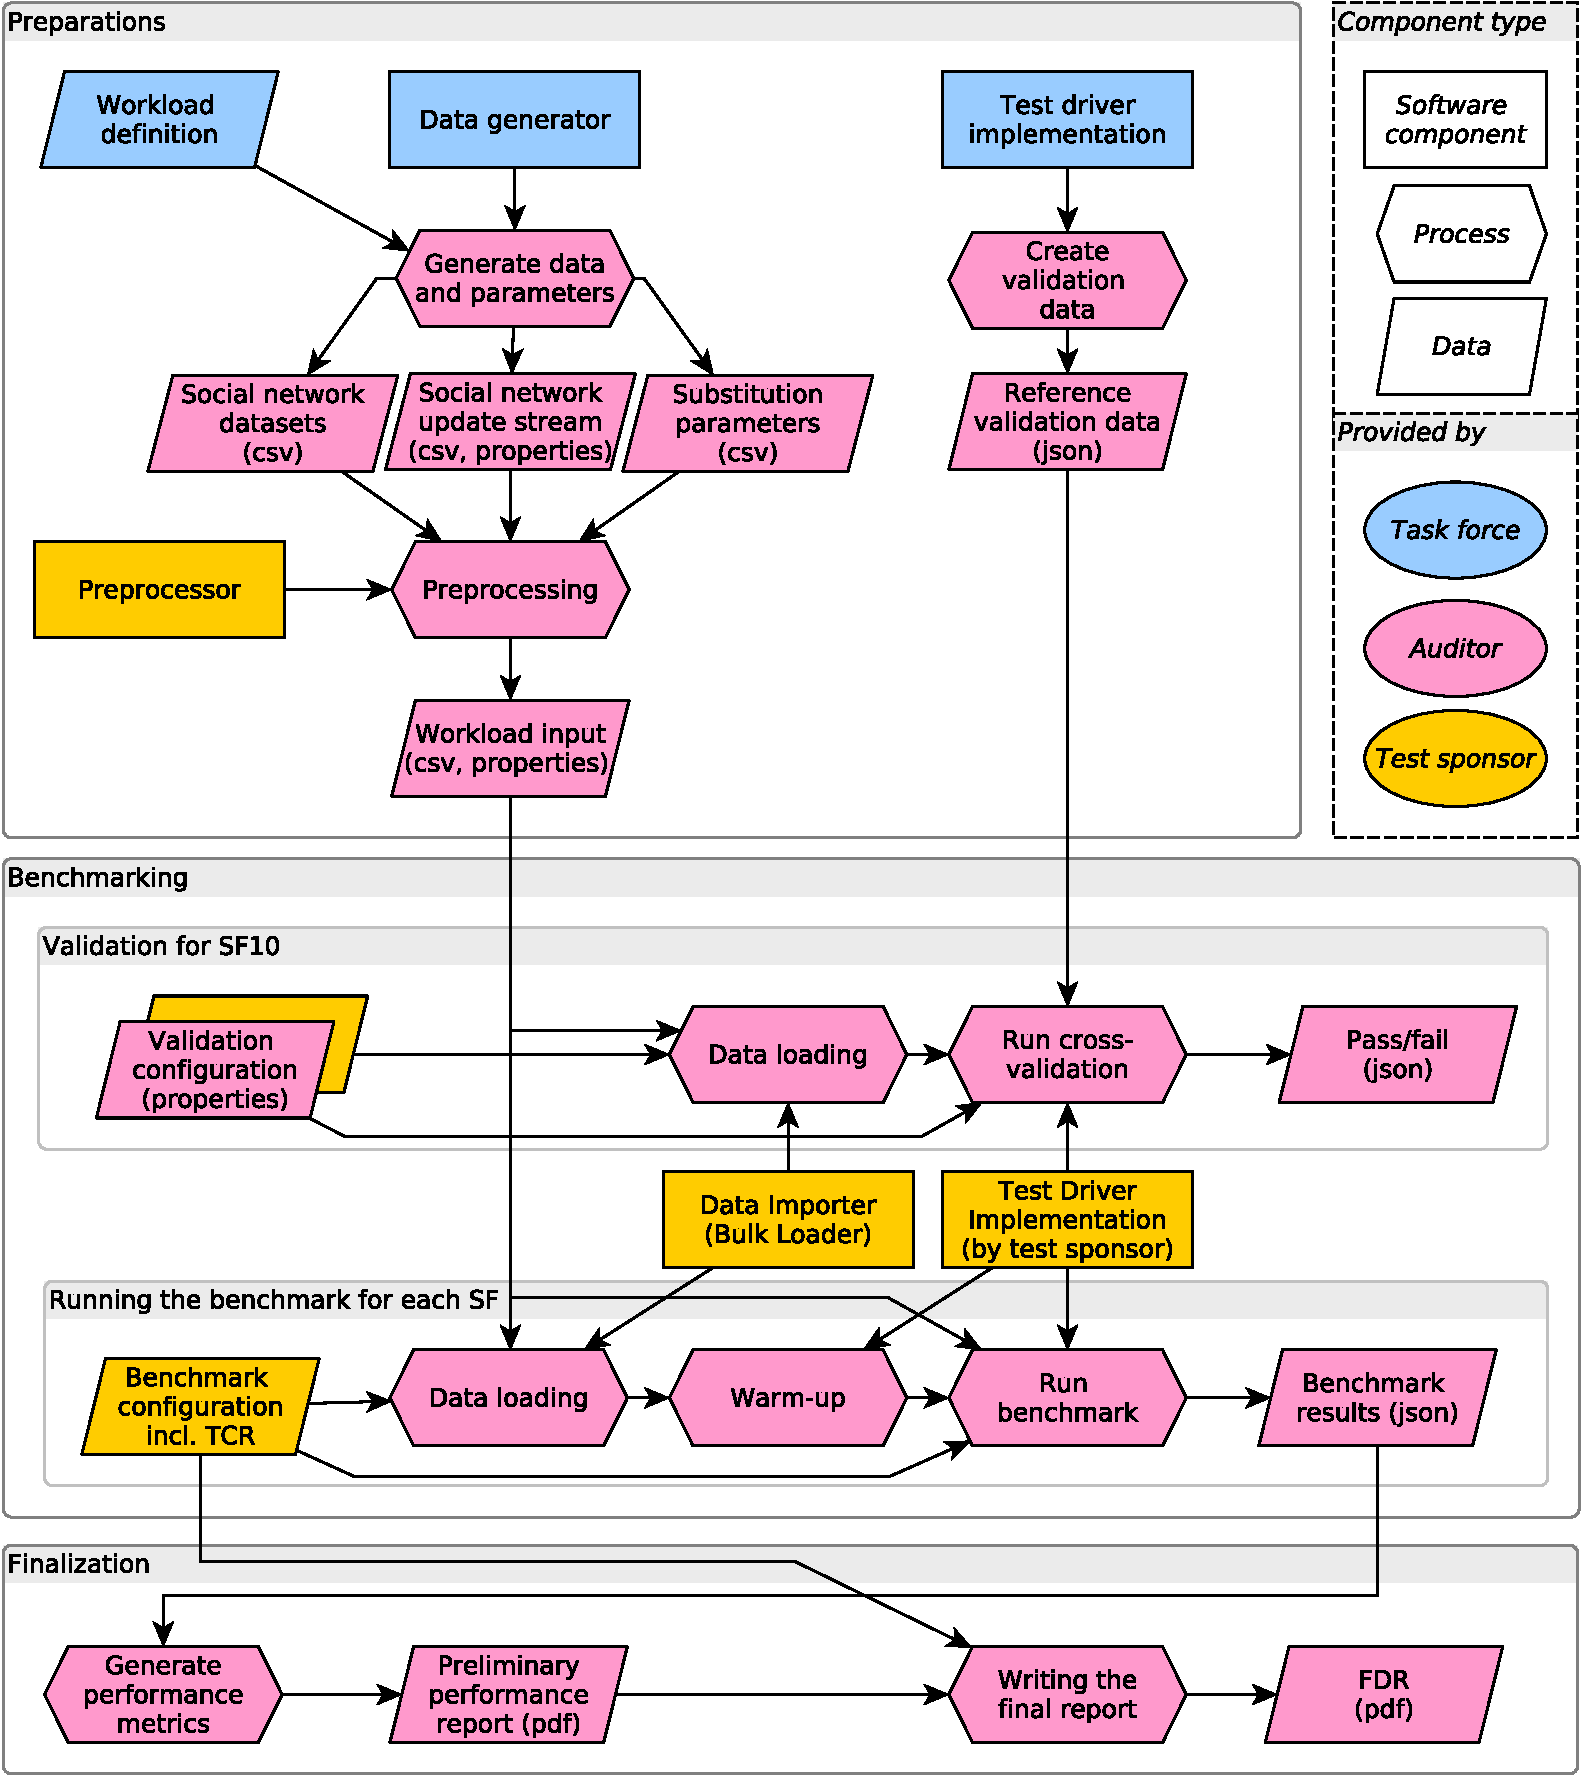
\includegraphics[scale=\yedscale]{figures/auditing-workflow}
    \caption{Benchmark execution and auditing workflow. For non-audited runs, the implementers perform the steps of the auditor.}
    \label{fig:audit-workflow}
\end{figure}

A key objective of the auditing guidelines for the Interactive workload is to \emph{allow a broad range of systems} to implement the benchmark.
Therefore, they do not impose constraints on the data model
(graph, relational, triple, \etc representations are allowed)
or on the query language
(both declarative and imperative languages are allowed).

\subsection{Scaling}
\label{sec:int-scaling}

\subsubsection{Scale Factors}

The scale factor of an SNB data set is the size of the data set in GiB of CSV (comma-separated values) files.
The size of a data set is characterized by scale factors: SF10, SF30, SF100 \etc (see \autoref{sec:scale-factors}).
All data sets contain data for three years of social network activity.

The \emph{validation run} shall be performed on the SF10 data set (see \autoref{sec:int-validation-data-set}) and use at least \numprint{100000} operations.
Note that the auditor may perform additional validation runs of the benchmark implementation using smaller data sets (\eg SF1) and issue queries.\footnote{%
An example test could be to issue complex reads with parameters such as \texttt{personId} and \texttt{messageId} selected from the \textsf{Person}/\textsf{Message} entities inserted from the update streams and cross-validate these against other systems. (The substitution parameters are taken from the initial snapshot of the graph so these nodes are not targeted by the regular workload executed by the driver.)%
}

Audited \emph{benchmark runs} of the Interactive workload shall use SF30 or larger data sets. The rationale behind this decision is to ensure that there is a sufficient number of update operations available to guarantee 2.5~hours of continuous execution (see \autoref{sec:int-measurement-window}).

% \begin{quote}
%     \emph{Rationale behind scaling.} The authors are aware that the prevalent practice for online benchmarks is to tie the reported throughput to the scale, \eg max 12.5 tpmC per warehouse in \mbox{TPC-C}. The authors depart from this practice here because with throughput tied to scale, test systems with interesting throughput rapidly become very expensive, raising the entry barrier for publishing a result. It is thought that scaling in buckets lowers the barrier of entry and reduces incentive to use hardware configurations that would be unusual in a production environment.
% \end{quote}
%COMMENTS FROM PAST GABOR TO FUTURE GABOR
%what it wants to say is that unlike TPC-C, you can get a large throughput (lots of ops) even on a small data set
%which is correct but we can ran out of updates due to the 2.5-hr simulation requirement
%so its (implied) conclusion does not hold fully hold for SNB interactive

\subsubsection{Social Network data sets}
\label{sec:int-data-sets}

\paragraph{Initial data set}
The data set is divided into a bulk loadable initial database population (90\%) and an update stream (10\%). These are generated by the SNB data generator. The data generator has options for splitting the data set into any number of files.

\paragraph{Dependencies between messages in the update stream}
The update stream contains the latest 10\% of the events in the simulated social network. These events form a single serializable sequence in time. Some events will depend on preceding events, for example a message must exist before a reply comment to the message is created. The data generator guarantees that these are separated by at least 10 seconds of simulation time.

\paragraph{Parallel updates}
The update stream may be broken into arbitrarily many sub-streams. The partition scheme is created by the \datagen. During benchmark execution, the driver preserves dependencies between update operations, such as ensuring not to refer to non-existent entities in updates (\eg a like is not added to a message which has not been inserted yet).

\subsection{Data Model and Data Loading}

\subsubsection{Supported Data Models}

SNB may be implemented with different data models (\eg relational, RDF, and different graph data models). The reference schema is provided in the specification using a UML-like notation. 


\subsubsection{Generated Input Data}
\label{sec:generated-data}

\paragraph{Storage}
The data generator produces comma-separated values (CSV) for all data models.

\paragraph{Data format}
A single attribute has a single data type, as follows:
\begin{description}
    \item [Identifier] This is an integer value foreign key or a URI in RDF. If this is an integer column, the implementation data type should support at least $2^{50}$ distinct values.
    \item [Date] A date should support a date range from 0000 to 9999 in the year field.
    \item [DateTime] A datetime should support a date range from 0000 to 9999 in the year field, with at least millisecond precision.
    \item [Short string] The string column for names may have a variable length and may have a declared maximum length, \eg 40 characters.
    \item [Long string] For example a message content may be a long string that is often short in the data but may not declare a maximum length and must support data sizes of up to 1~MB.
\end{description}

The above is stated in further detail in the benchmark specification, and it shall take precedence over the
above in the case of conflict.

A single attribute in the reference schema may not be divided into multiple attributes in the target schema.

\paragraph{Database schema}
A schema on the DBMS is optional. An RDF implementation for example may work without one. An RDF implementation is allowed to load the RDF reference schema and to take advantage of the data type and cardinality statements therein. 

\paragraph{Configuration parameters}
\datagen configuration parameters, including SF, distributions, number of persons, serialiser (\eg CsvSingularMergedFK) should be reported.

\paragraph{Primary data structures}
An RDF, relational, or graph schema may specify system specific options affecting DBMS storage layout. These may for example specify vertical partitioning. Vertical partitioning means anything from a column store layout with per-column allocated storage space to use of explicit column groups. Any mix of row or column-wise storage structures is allowed as long as this is declaratively specified on a per data structure-basis.

\paragraph{Auxiliary data structures}
Covering indices and clustered indices are allowed. If these are defined, then all replications of data implied by these must be maintained statement by statement, \ie each auxiliary data structure must be consistent with any other data structures of the table after each data manipulation operation.

A covering index is an index which materialises a specific order of a specific subset or possibly all columns of a table. 
A clustered index is an index which materialises all columns of a table in a specific order, which order may or may not be that of the primary key of the table. A clustered or covering index may be the primary or only representation of a table.

Any subset of the columns on a covering or clustered index may be used for ordering the data. A hash based index or a combination of a hash based and tree based index are all allowed, in row or column-wise or hybrid forms.

\paragraph{Loading the data}

We expect the SUT to provide some means to bulk load the data set either in the form of a dedicated offline loader component or an online loader that allows bulk inserting into a database.
The total of the bulk load time and the time for subsequent operations (indexing, computing statistics, \etc) must be reported in the FDR (see \autoref{sec:int-benchmark-workflow}).
As loading can be an expensive operation, it is allowed to conduct the audit such that the loading is only performend once, and the validation/benchmarking phases use the resulting database instance.
In practice, this can look like as follows:
(1)~load the data,
(2)~compute statistics, uniqueness constraints, keys, indices, \etc,
(3)~shut down the SUT,
(4)~create a backup of the database (\eg by copying the directory of the database).
For all subsequent runs, the database shall be restored from the backup.

\subsection{Precomputation}

Precomputation of query results (both interim and end results) is allowed. However, systems must ensure that precomputed results (\eg materialized views) are kept consistent upon updates.

\subsection{Benchmark Software Components}
\label{sec:snb-software-components}
LDBC provides a test driver, data generator, and summary reporting scripts. Benchmark implementations shall use a stable version (\eg 0.3.6) of the test driver. The SUT's database software should be a stable version that is available publicly or can be purchased at the time of the release of the audit.

\subsubsection{Adaptation of the Test Driver to a DBMS}
\label{sec:test-driver}
A qualifying run must use a test driver that adapts the provided test driver to interface with the SUT. Such an implementation, if needed, must be provided by the test sponsor. The parameter generation, result recording, and workload scheduling parts of the test driver should not be changed. The auditor must be given access to the test driver source code used in the reported run.

The test driver produces the following artefacts for each execution as a by product of the run: Start and end timestamps in wall clock time, recorded with microsecond precision. The identifier of the operation and any substitution parameters.


\subsubsection{Summary of Benchmark Results}
\label{sec:performance-metrics}
A separate test summary tool provided with the test driver analyses the test driver log(s) after a measurement window is completed. 

The tool produces for each of the distinct queries and transactions the following summary:
\begin{itemize}
    \item Run time of query in wall clock time.
    \item Count of executions.
    \item Minimum/mean/percentiles/maximum execution time.
    \item Standard deviation from the average execution time.
\end{itemize}
The tool produces for the complete run the following summary:
\begin{itemize}
    \item Operations per second for a given SF (throughput). This is the primary metric of this workload.
    \item The total execution time in wall clock time.
    \item The total number of completed operations.
\end{itemize}


\subsection{Implementation Language and Data Access Transparency}

The queries and updates may be implemented in a domain-specific query language or as procedural code written in a general-purpose programming language (\eg using the API of the database).

\subsubsection{Implementations Using a Domain-Specific Query Language}
\label{sec:snb-domain-specific-query-language}

If a domain-specific query language is used, \eg SPARQL, SQL, Cypher, or Gremlin, then explicit query plans are prohibited in all the read-only queries.%
\footnote{If the queries are not clearly declarative, the auditor must ensure that they do not specify explicit query plans by investigating their source code and experimenting with the query planner of the system (\eg using SQL's \texttt{EXPLAIN} command).}
The update transactions may still consist of multiple statements, effectively amounting to explicit plans.

Explicit query plans include but are not limited to:
\begin{itemize}
    \item Directives or hints specifying a join order or join type
    \item Directives or hints specifying an access path, \eg which index to use
    \item Directives or hints specifying an expected cardinality, selectivity, fanout or any other information that pertains to the expected number or results or cost of all or part of the query.
\end{itemize}

\begin{quote}
    \emph{Rationale behind the applied restrictions.} The updates are effectively OLTP and, therefore, the customary freedoms apply, including the use of stored procedures, however subject to access transparency. Declarative queries in a benchmark implementation should be such that they could plausibly be written by an application developer. Therefore, their formulation should not contain system specific aspects that an application developer would be unlikely to know. In other words, making a benchmark implementation should not require uncommon sophistication on behalf of the developer. This is regular practice in analytical benchmarks, \eg \mbox{TPC-H}.
\end{quote}

\subsubsection{Implementations Using a General-Purpose Programming Language}
\label{sec:snb-general-purpose-programming-language}

Implementations using a general-purpose programming language for specifying the queries (including procedural, imperative, and API-based implementations) are expected to respect the rules described in \autoref{sec:query-languages}.
For these implementations, the rules in \autoref{sec:snb-domain-specific-query-language} do not apply.

\subsection{Correctness of Benchmark Implementation}

\subsubsection{Validation data set}
\label{sec:int-validation-data-set}
The scale factor 10 shall be used as validation data set.

\subsubsection{ACID Compliance}
\label{sec:int-acid-compliance}

The Interactive workload requires full ACID support (\autoref{sec:acid-compliance}) from the SUT.
This is tested using the LDBC ACID test suite.
For the specification of this test suite, see \autoref{sec:acid-test-suite} and the related software repository at \url{https://github.com/ldbc/ldbc_acid}.

\paragraph{Expected level of isolation}
If a transaction reads the database with intent to update, the DBMS must guarantee that repeating the same read within the same transaction will return the same data. This also means that no more and no less data rows must be returned. In other words, this corresponds to snapshot or to serializable isolation. If the database is accessed without transaction context or without intent to update, then the DBMS should provide read committed semantics, \eg repeating the same read may produce different results but these results may never include effects of pending uncommitted transactions.

\paragraph{Durability and checkpoints}

A checkpoint is defined as the operation which causes data persisted in a transaction log to become durable outside of the transaction log. Specifically, this means that an SUT restart after instantaneous failure following the completion of the checkpoint may not have recourse to transaction log entries written before the end of the checkpoint.

A checkpoint typically involves a synchronisation barrier at which all data committed prior too the moment is required to be in durable storage that does not depend on the transaction log.
Not all DBMSs use a checkpointing mechanism for durability. For example a system may rely on redundant storage of data for durability guarantees against instantaneous failure of a single server.

The measurement window may contain a checkpoint. If the measurement window does not contain one, then the restart test will involve redoing all the updates in the window as part of the recovery test.

The timed window ends with an instantaneous failure of the SUT. Instantaneously killing all the SUT process(es) is adequate for simulating instantaneous failure. All these processes should be killed within one second of each other with an operating system action equivalent to the Unix \verb+kill -9+. If such is not available, then powering down each separate SUT component that has an independent power supply is also possible.

The restart test consists of restarting the SUT process(es) and finishes when the SUT is back online with all its functionality and the last successful update logged by the driver can be seen to be in effect in the database.
%In the case of a distributed (scale-out) system, a particular partition may be recovered whereas another one is still in the process of recovering. If this is so, then checking for the last update shall not be done until all partitions are online.

If the SUT hardware was powered down, the recovery period does not include the reboot and possible file system check time. The recovery time starts when the DBMS software is restarted.




\paragraph{Recovery} 
The SUT is to be restarted after the measurement window and the auditor will verify that the SUT contains the entirety of the last update recorded by the test driver(s) as successfully committed. The driver or the implementation have to make this information available. The auditor may also check the \emph{audit log} of the SUT (if available) to confirm that the operations issued by the driver were saved.

Once an official run has been validated, the recovery capabilities of the system must be tested. The system and the driver must be configured in the same way as in during the benchmark execution. After a warm-up period, an execution of the benchmark will be performed under the same terms as in the previous measured run.

\paragraph{Measuring recovery time}
At an arbitrary point close to 2 hours of wall clock time during the run, the machine will be shut down. Then, the auditor will restart the database system and will check that the last committed update (in the driver log file) is actually in the database. The auditor will measure the time taken by the system to recover from the failure. Also, all the information about how durability is ensured must be disclosed. If checkpoints are used, these must be performed with a period of 10 minutes at most.


\subsection{Benchmarking Workflow}
\label{sec:int-benchmark-workflow}

A benchmark execution is divided into the following processes (these processes are also shown in \autoref{fig:audit-workflow}):

\begin{description}
    \item[Generate data] This includes running the data generator, placing the generated files in a staging area, configuring storage, setting up the SUT configuration and preparing any data partitions in the SUT. This may include preallocating database space but may not include loading any data or defining any schema having to do with the benchmark. The \verb|ldbc.snb.interactive.update_interleave| driver parameter must come from the \verb|updateStream.properties| file, which is created by the data generator. That parameter should never be set manually. This parameter signifies the average distance of update operations in the workload.
    \item[Preprocessing] If needed, the output from the data generator is to preprocess the data set (\autoref{sec:auditing-data-format}).
    \item[Create validation data] Using one of the reference implementations of the benchmark, the reference validation data is obtained in .json format.
    \item[Data loading] The test sponsor must provide all the necessary documentation and scripts to load the data set into the database to test.
    This includes defining the database schema, if any, loading the initial database population, making this durably stored and gathering any optimiser statistics.
    The system under test must support the different data types needed by the benchmark for each of the attributes at their specified precision. No data can be filtered out, everything must be loaded. The test sponsor must provide a tool to perform arbitrary checks of the data or a shell to issue queries in a declarative language if the system supports it.
    \item[Run cross-validation] This step uses the data loader to populate the database, but the load is not timed. The validation data set is used to verify the correctness of the SUT. The auditor must load the provided data set and run the driver in validation mode, which will test that the queries provide the official results.  The benchmarking workflow will not go beyond this point unless results match the expected output.
    \item[Warm-up] Benchmark runs are preceded by a warm-up which must be performed using the LDBC driver.
    \item[Run benchmark] The bulk load time is reported and is equal to the amount of elapsed wall clock time between starting the schema definition and receiving the confirmation message of the end of statistics gathering. The workflow runs begin after the bulk load is completed. If the run does not directly follow the bulk load, it must start at a point in the update stream that has not previously been played into the database. In other words, a run may only include update events whose timestamp is later than the latest message creation date in the database prior to start of run. The run starts when the first of the test drivers send its first message to the SUT. If the SUT is running in the same process as the driver, the window starts
    when the driver starts. Also, make sure that the \verb|-rl/--results_log| is enabled. Make sure that all operations are enabled and the frequencies are those for the selected scale factor (see the exact specification of the frequencies in \autoref{sec:sf-statistics}).
\end{description}

\subsubsection{Query Timing During Benchmark Run}
\label{sec:ontime-requirements}
A valid benchmark run must last at least 2 hours of wall clock time and at most 2 hours and 15 minutes.
In order to be valid, a benchmark run needs to meet the ``95\% on-time requirement''.
The \texttt{results\_log.csv} file contains the $\mathsf{actual\_start\_time}$ and the $\mathsf{scheduled\_start\_time}$ of each of the issued queries. In order to have a valid run, 95\% of the queries must meet the following condition:
\begin{equation*}
\mathsf{actual\_start\_time} - \mathsf{scheduled\_start\_time} < 1\
\mathrm{second}
\end{equation*}

If the execution of the benchmark is valid, the auditor must retrieve all the files from directory specified by \verb|--results_dir| which includes configuration settings used, results log and results summary. All of which must be disclosed.

\subsubsection{Measurement Window}
\label{sec:int-measurement-window}

Benchmark runs execute the workload on the SUT in two phases (\autoref{fig:measurement-window-selection}).
First, the SUT must undergo a warm-up period that takes at least 30 minutes and at most 35 minutes. The goal of this is to put the system in a steady state which reflects how it would behave in a normal operating environment. The performance of the operations during warm-up is not considered.
Next, the SUT is benchmarked during a two-hour measurement window. Operation times are recorded and checked to ensure the ``95\% on-time requirement'' is satisfied.

\begin{figure}[h]
    \centering
    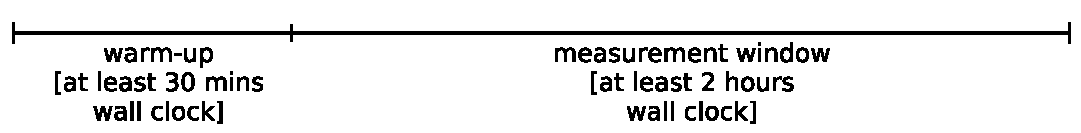
\includegraphics[width=.7\linewidth]{figures/measurement-window-selection}
    \caption{Warm-up and measurement window for benchmark run.}
    \label{fig:measurement-window-selection}
\end{figure}

The SNB \datagen produces 3~years worth data of which 10\% is used for updates (\autoref{sec:int-data-sets}), \ie approximately $3 \times 365 \times 0.1 = 109.5~\text{days} = 2628~\text{hours}$.
To ensure that the 2.5~hour wall clock period has enough input data, the lower bound of TCR is defined as 0.001 (if $2628$ hours of updates are played back at more than $1000\times$ speed, the benchmark framework runs out of updates to execute). System that can achieve a better compression (\ie lower TCR value) on a given scale factor should use larger SFs for their benchmark runs -- otherwise their total runs will be less than 2.5~hours, making them unsuitable for auditing.

%The test summary tool may be used for reading the logs created by a test driver.

\subsection{Full Disclosure Report}
\label{sec:int-fdr}

Upon successful completion of the audit, an FDR is compiled. In addition to the general requirements, the full disclosure shall cover the following:

\begin{itemize}
    \item General terms: an executive summary and declaration of the credibility of the audit
    \item System description and pricing summary: see \autoref{sec:system-config}
    \item Data generation and data loading: see \autoref{sec:generated-data}
    \item Test driver details: see \autoref{sec:test-driver}
    \item Performance metrics: see \autoref{sec:performance-metrics}
    \item Validation results: see \autoref{sec:int-validation-data-set}
    \item ACID compliance: see \autoref{sec:acid-compliance}
    \item List of supplementary materials
\end{itemize}

To ensure reproducibility of the audited results, a supplementary package is attached to the full disclosure report. This package should contain:

\begin{itemize}
    \item A README file with instructions specifying how to set up the system and run the benchmark
    \item Configuration files of the database, including database-level configuration such as buffer size and schema descriptors (if necessary)
    \item Source code or binary of a generic driver that can be used to interact with the DBMS
    \item SUT-specific LDBC driver implementation (similarly to the projects in \url{https://github.com/ldbc/ldbc_snb_interactive_v1_impls}, \url{https://github.com/ldbc/ldbc_snb_interactive_v2_impls}, \url{https://github.com/ldbc/ldbc_snb_bi})
    \item Script or instructions to compile the LDBC Java driver implementation
    \item Instructions on how to the reach the server through CLI and/or web UI (if applicable), \eg the URL (including port number), user name and password
    \item LDBC configuration files (\texttt{.properties}), including the \texttt{time\_compression\_ratio} values used in the audited runs
    \item Scripts to preprocess the input files (if necessary) and to load the data sets into the database
    \item Scripts to create validation data sets and to run the benchmark
    \item The implementations of the queries and the update operations, including their complete source code (\eg declarative queries specifications, stored procedures, \etc)
    \item Implementation of the ACID test suite
    \item Binary package of the DBMS (\eg \texttt{.deb} or \texttt{.rpm})
\end{itemize}



%%%%%%%%%%%%%%%%%%%%%%%%%%%%%%%%%%%%%%%%%%%%%%%%%%%%%%%%%%%%%%%%%%%%%%%%%%%%%%
%%%%%%%%%%%%%%%%%%%%%%%%%%%%%%%%%%%%%%%%%%%%%%%%%%%%%%%%%%%%%%%%%%%%%%%%%%%%%%
%%%%%%%%%%%%%%%%%%%%%%%%%%%%%%%%%%%%%%%%%%%%%%%%%%%%%%%%%%%%%%%%%%%%%%%%%%%%%%

\section{Auditing Rules for the Business Intelligence Workload}
\label{sec:auditing-bi-workload-audit}

%%%%%%%%%%%%%%%%%%%%%%%%%%%%%%%%%%%%%%%%%%%%%%%%%%%%%%%%%%%%%%%%%%%%%%%%%%%%%%
%%%%%%%%%%%%%%%%%%%%%%%%%%%%%%%%%%%%%%%%%%%%%%%%%%%%%%%%%%%%%%%%%%%%%%%%%%%%%%
%%%%%%%%%%%%%%%%%%%%%%%%%%%%%%%%%%%%%%%%%%%%%%%%%%%%%%%%%%%%%%%%%%%%%%%%%%%%%%

The following section describes the auditing rules specific to the Business Intelligence (BI) workload.

\subsection{Overview}
\label{sec:auditing-bi-audit-overview}

Implementing the BI workload requires the following key capabilities:

\begin{itemize}
    \item Loading the initial snapshot of the social network graph
    \item Evaluating the BI read queries (\autoref{sec:bi-reads})
    \item Evaluating the BI write operations: inserts (\autoref{sec:bi-insert-operations}) and deletes (\autoref{sec:bi-delete-operations})
    \item Performing concurrent reads and writes (\autoref{sec:auditing-bi-audit-workflow}) (optional, only allowed if ACID compliance is guaranteed)
\end{itemize}

\subsection{Workflow}
\label{sec:auditing-bi-audit-workflow}

\begin{figure}[htbp]
    \centering
    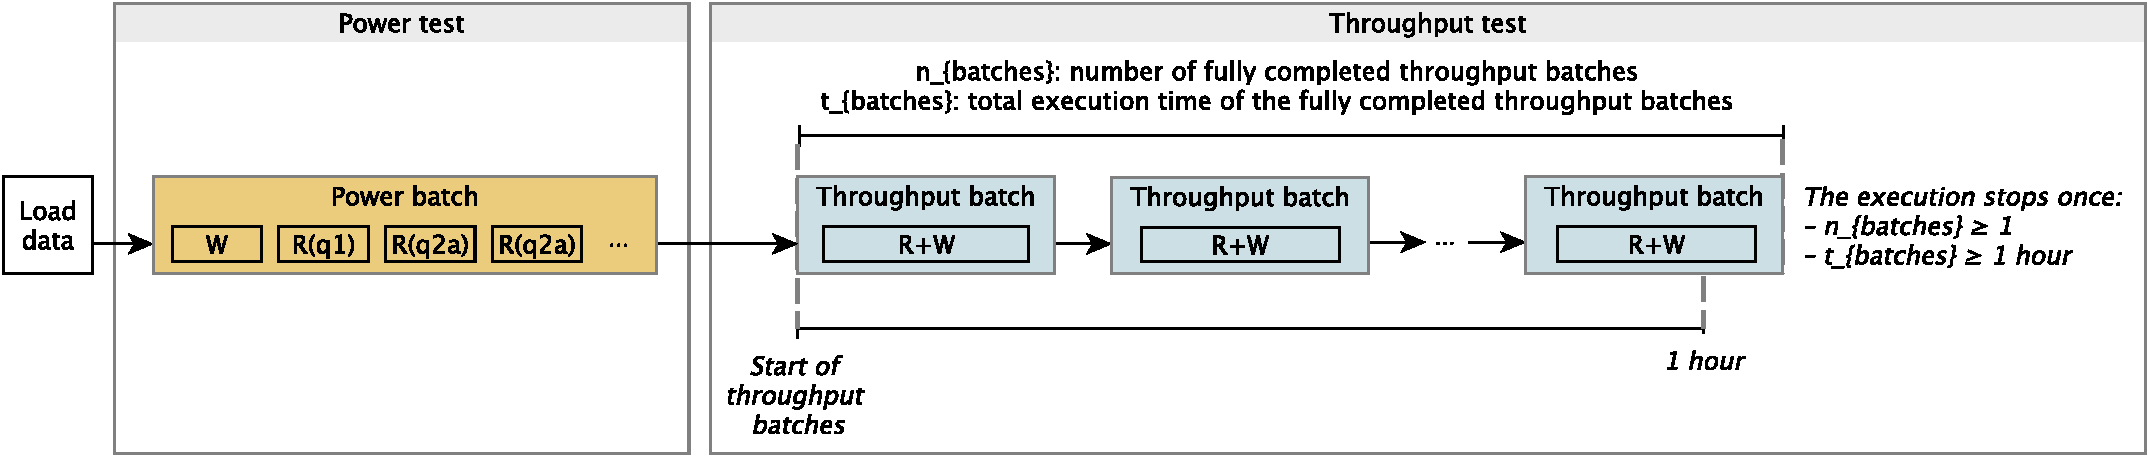
\includegraphics[scale=\yedscale]{figures/bi-batches.pdf}
    \caption{Tests and batches (power and throughput) executed in the BI workload's workflow.}
    \label{fig:bi-batches}
\end{figure}

The write operations and read queries are run in \emph{daily batches}.
In each batch, each query variant
(Q1, Q2\variantA, Q2\variantB, Q3, \ldots, Q20\variantA, Q20\variantB)
is executed using 30~different substitution parameters.
The BI workflow (\autoref{fig:bi-batches}) consists of two key parts:
the \emph{power test} (\autoref{sec:power-test}) and
the \emph{throughput test} (\autoref{sec:throughput-test}).

\subsubsection{Power Test}
\label{sec:power-test}

The \emph{power test} runs a single \emph{power batch}. This test first runs the write operations, followed by a sequential execution of individual read query variants.
The writes perform a day of inserts and deletes in the simulated social network,
while a total of $28 \times 30 = 840$ read queries are executed.

\subsubsection{Throughput Test}
\label{sec:throughput-test}

The \emph{throughput test} consists of multiple \emph{throughput batches}.
Each throughput batch runs the same type and the same amount of operations as the power batch.
However, they allow concurrent execution of the write operations and read queries in a given batch.

The execution of the throughput test during audits is the \emph{throughput measurement window}.
This window must span at least for 1~hour and
it must include at least one fully completed batch (see \autoref{fig:bi-batches}).

The workload defines two execution modes for the \emph{throughput batches}:

\begin{description}
    \item[Disjoint RW mode]
    In \emph{disjoint RW (read-write) mode} the system performs the reads and writes separately. It first executes the writes, then evaluates the read queries. Concurrency between the read operations is allowed.\\
    This mode is aimed at \emph{read-optimized data analytical systems} which do not support concurrent reads and writes. Implementations may also opt to use this mode for simplicity. For these implementations, passing the \emph{LDBC ACID compliance test} (\autoref{sec:acid-test-suite}) is not required.

    \item[Concurrent RW mode]
    In \emph{concurrent RW (read-write) mode} the system is allowed to run reads and writes concurrently. This requires the systems to be capable of handling \emph{transactions}. Implementations using this mode are required to pass the \emph{LDBC ACID compliance test} (\autoref{sec:acid-test-suite}).
\end{description}

\subsection{Runtimes}

The runtimes should be reported as follows:

\begin{itemize}
    \item The \emph{load time} ($t_\textit{load}$) denotes the time to load the data into the SUT and initialize auxiliary data structures (if applicable). For audited runs, we require that $t_\textit{load} < 24\textrm{ hours}$.
    \item The \emph{power test time} ($t_\textit{power test}$) denotes the time to perform the power test.
    \item The \emph{throughput measurement window time} ($t_\textit{throughput\ measurement}$) denotes the time to perform the throughput test, including the last (potentially unfinished) batch.
    \item The \emph{full throughput batches time} ($t_\textit{full\ throughput\ batches}$) denotes the time to evaluate the fully completed batches during the throughput measurement window.
\end{itemize}

Note that a warm-up period is not allowed (unlike the Interactive workload where such a period is required, see \autoref{sec:int-measurement-window}).

\subsection{Scoring Metrics}
\label{sec:auditing-bi-scoring-metrics}

SNBI BI provides four scoring metrics:
the \emph{power score}, the \emph{throughput score}, and their price-adjusted variants,
the \emph{per-\$ power score} and the \emph{per-\$ throughput score}.
All scores include the scale factor, denoted with ``@SF''.

\subsubsection{Price}
\label{sec:price-metrics}

We follow TPC's specification for reporting prices~\cite{tpc-pricing}.
The price is established as the \emph{total cost of ownership ($\textit{TCO}$)} for the SUT used in the benchmark,
reported as a breakdown of
machine cost,
software license costs,
and maintenance costs for 3 years.
In case of cloud deployments, the cost of running a 3-year reserved instance should be reported.
When establishing the price, the ``upfront payment'' option available at certain cloud providers should not be considered.

\subsubsection{Power Scores}
\label{sec:power-score}

The definition of \snbbi's power score follows \tpcH in using a geometric mean, ensuring that there is an incentive to improve all queries, no matter their running time.
Formally, the power score is based on the time to perform the writes
and
the time spent for executing each variant with 30~different substitution parameters, measured in seconds:
$$
\textit{power@SF} =
    \frac{\numprint{3600}}{\sqrt[29]{
        w
        \cdot q_{1}
        \cdot q_{2\variant{a}}
        \cdot q_{2\variant{b}}
        \cdot \ldots
        \cdot q_{18}
        \cdot q_{19\variant{a}}
        \cdot q_{19\variant{b}}
        \cdot q_{20\variant{a}}
        \cdot q_{20\variant{b}}
    }}
    \cdot
    \textit{SF}
$$

% Including all entries, the formula is:
% {\scriptsize
% $$
% \textit{power@SF} =
%     \frac{\numprint{3600}}{\sqrt[29]{
%         w
%         \! \cdot \! q_{1}
%         \! \cdot \! q_{2\variant{a}}
%         \! \cdot \! q_{2\variant{b}}
%         \! \cdot \! q_{2\variant{a}}
%         \! \cdot \! q_{2\variant{b}}
%         \! \cdot \! q_{3}
%         \! \cdot \! q_{4}
%         \! \cdot \! q_{5}
%         \! \cdot \! q_{6}
%         \! \cdot \! q_{7}
%         \! \cdot \! q_{8\variant{a}}
%         \! \cdot \! q_{8\variant{b}}
%         \! \cdot \! q_{9}
%         \! \cdot \! q_{10\variant{a}}
%         \! \cdot \! q_{10\variant{b}}
%         \! \cdot \! q_{11}
%         \! \cdot \! q_{12}
%         \! \cdot \! q_{13}
%         \! \cdot \! q_{14\variant{a}}
%         \! \cdot \! q_{14\variant{b}}
%         \! \cdot \! q_{15\variant{a}}
%         \! \cdot \! q_{15\variant{b}}
%         \! \cdot \! q_{16\variant{a}}
%         \! \cdot \! q_{16\variant{b}}
%         \! \cdot \! q_{17}
%         \! \cdot \! q_{18}
%         \! \cdot \! q_{19\variant{a}}
%         \! \cdot \! q_{19\variant{b}}
%         \! \cdot \! q_{20\variant{a}}
%         \! \cdot \! q_{20\variant{b}}
%     }}
%     \cdot
%     \textit{SF}
% $$
% }

To determine the price-adjusted power score, we factor in the $\textit{TCO}$\emph{:}
$$ \textit{power@SF/\$} = \textit{power@SF} \cdot \frac{\numprint{1000}}{\textit{TCO}} $$

\subsubsection{Throughput Scores}
\label{sec:throughput-score}

The throughput score is based on $t_\textit{load}$, measured in hours,
and the cumulative execution time and number of the throughput batches executed:
%throughput score is calculated as the number of batches the system could execute in a single day
$$
\textit{throughput@SF} =
    (24\text{ hours} - t_\textit{load})
    \cdot
    \frac{n_\textit{batches}}{t_\textit{batches}}
    \cdot
    \textit{SF}
$$

The subtraction of $t_\textit{load}$ ensures that the scoring rewards systems with efficient bulk loaders (unlike in \tpcH and \tpcDS which do not include load performance in their metrics).
The price-adjusted throughput score is determined analogously: % to the price-adjusted power score.
$$ \textit{throughput@SF/\$} = \textit{throughput@SF} \cdot \frac{\numprint{1000}}{\textit{TCO}} $$

\subsection{Implementation Rules}
\label{sec:auditing-bi-implementation-rules}

\subsubsection{Correctness}
\label{sec:auditing-bi-correcntess}

The SUT shall evaluate all operators correctly.
The auditor shall ascertain correctness on the SF10 data set. However, they are allowed to also use data sets of different scale factors, as well as issue custom operations (both reads and writes) to test for the correctness of the implemenation.

The validation of correctness is performed on the output of the \emph{power test} step.
The rationale for using this only step is that during concurrent execution of R/W operations in the \emph{throughput test}, it is not possible to guarantee deterministic query results, making validation impossible. Moreover, this step already includes a write batch, therefore the query results indirectly test the correctness of the implementation of write operations.

\subsubsection{Auxiliary Data Structures}
\label{sec:auditing-bi-auxiliary-data-structures}

Using auxiliary data structures (\eg indices, materialized views) is allowed if they are kept in an up-to-date state after each write operation. The full disclosure report should enumerate the auxiliary data structures used by the SUT. 

\subsubsection{Query Declarativity}
\label{sec:auditing-bi-query-declarativity}

Systems should use a domain-specific query language (\eg Cypher, Gremlin, GSQL) for the implementation, including the read queries and the update operations.
General-purpose programming languages (\eg C, C\texttt{++}, Java, Julia) are not allowed.

Implementations shall not use \emph{query-specific stored procedures written in a general-purpose programming language} (\eg a given procedure which implements BI Q5).
Using the stored procedure libraries considered to be the ``standard libraries'' of the SUT is allowed.%
\footnote{These libraries often include features such as weighted shortest path algorithms.}
Implementations may use \emph{stored procedures written in a domain-specific language}.
In cases when the categorization of the approach used by the SUT's query implementations is uncertain, it is the auditor's responsibility to decide whether the SUT complies with this rule.

\subsubsection{Query Variants}
\label{sec:auditing-bi-query-variants}

Several queries (\eg \queryRefCard{bi-read-14}{BI}{14}) use \variantA and \variantB variants with different sets of input parameters.
The SUT should not receive any hints on which variant it is currently evaluating (\eg Q14\variantA or Q14\variantB).
Moreover, it is not allowed for the query implementations to contain code that aims to detect the query variant used.

\subsection{Scaling}
\label{sec:auditing-bi-scaling}

Audited \emph{benchmark runs} of the BI workload shall use SF30 or larger data sets.
The rationale behind this decision is to ensure that there should be a sufficient number of write operations available to guarantee the execution during the duration of the measurement window (see \autoref{fig:bi-batches}).

\subsection{Full Disclosure Report}
\label{sec:auditing-bi-fdr}

The \emph{full disclosure report} (FDR) and the \emph{supplementary package} shall contain
the same information as for SNB Interactive (\autoref{sec:int-fdr}),
including, if applicable (\autoref{sec:auditing-bi-implementation-rules}), the ACID compliance report (\autoref{sec:acid-compliance}).




%%%%%%%%%%%%%%%%%%%%%%%%%%%%%%%%%%%%%%%%%%%%%%%%%%%%%%%%%%%%%%%%%%%%%%%%%%%%%%
%%%%%%%%%%%%%%%%%%%%%%%%%%%%%%%%%%%%%%%%%%%%%%%%%%%%%%%%%%%%%%%%%%%%%%%%%%%%%%
%%%%%%%%%%%%%%%%%%%%%%%%%%%%%%%%%%%%%%%%%%%%%%%%%%%%%%%%%%%%%%%%%%%%%%%%%%%%%%



\chapter{Auditing rules}\label{chapter:auditing}
\chapter{Auditing Policies}
\label{sec:auditing}

\emph{This chapter contains the auditing policies for the LDBC Social Network Benchmark. The initial draft of the auiting policies were published in the EU project deliverable D6.3.3 ``LDBC Benchmark Auditing Policies''.}

%%%%%%%%%%%%%%%%%%%%%%%%%%%%%%%%%%%%%%%%%%%%%%%%%%%%%%%%%%%%%%%%%%%%%%%%%%%%%%
%%%%%%%%%%%%%%%%%%%%%%%%%%%%%%%%%%%%%%%%%%%%%%%%%%%%%%%%%%%%%%%%%%%%%%%%%%%%%%
%%%%%%%%%%%%%%%%%%%%%%%%%%%%%%%%%%%%%%%%%%%%%%%%%%%%%%%%%%%%%%%%%%%%%%%%%%%%%%

This chapter is divided in the following parts:
\begin{itemize}
    \item Motivation of benchmark result auditing
    \item General discussion of auditable aspects of benchmarks
    \item Specific checklists and running rules for the Social Network Benchmark's workloads (Interactive, Business Intelligence)
\end{itemize}

Many definitions and general considerations are shared between the benchmarks, hence it is justified to present the principles first and to refer to these in the context of the benchmark specific rules.

The auditing process, including the auditor certification exams, the possibility of challenging audited results, \etc, are defined in the LDBC Byelaws~\cite{ldbc_byelaws}. Please refer to the latest Byelaws document when conducting audits.

%%%%%%%%%%%%%%%%%%%%%%%%%%%%%%%%%%%%%%%%%%%%%%%%%%%%%%%%%%%%%%%%%%%%%%%%%%%%%%
%%%%%%%%%%%%%%%%%%%%%%%%%%%%%%%%%%%%%%%%%%%%%%%%%%%%%%%%%%%%%%%%%%%%%%%%%%%%%%
%%%%%%%%%%%%%%%%%%%%%%%%%%%%%%%%%%%%%%%%%%%%%%%%%%%%%%%%%%%%%%%%%%%%%%%%%%%%%%

\section{Rationale and General Principles}

%%%%%%%%%%%%%%%%%%%%%%%%%%%%%%%%%%%%%%%%%%%%%%%%%%%%%%%%%%%%%%%%%%%%%%%%%%%%%%
%%%%%%%%%%%%%%%%%%%%%%%%%%%%%%%%%%%%%%%%%%%%%%%%%%%%%%%%%%%%%%%%%%%%%%%%%%%%%%
%%%%%%%%%%%%%%%%%%%%%%%%%%%%%%%%%%%%%%%%%%%%%%%%%%%%%%%%%%%%%%%%%%%%%%%%%%%%%%

The purpose of benchmark auditing is to improve the \emph{credibility} and \emph{reproducibility} of benchmark claims by involving a set of detailed execution rules and third party verification of compliance with these.

Rules may exist separately of auditing but auditing is not meaningful unless the rules are adequately precise.
Aspects like auditor training and qualification cannot be addressed separately from a discussion of the matters the
auditor is supposed to verify. Thus the credibility of the entire process hinges on clear and shared understanding
of what a benchmark is expected to demonstrate and on the auditor being capable of understanding the process
and of verifying that the benchmark execution is fair and does not abuse the rules or pervert the objectives of
the benchmark.

Due to the open-ended nature of technology and the agenda of furthering innovation via measurement, it is
not feasible or desirable to over-specify the limits of benchmark implementation. Hence there will always remain
judgement calls for borderline cases. In this respect auditing and the LDBC are not separate. It is expected that
issues of compliance as well as of maintenance of rules will come before the LDBC as benchmark claims are
made.

%%%%%%%%%%%%%%%%%%%%%%%%%%%%%%%%%%%%%%%%%%%%%%%%%%%%%%%%%%%%%%%%%%%%%%%%%%%%%%
%%%%%%%%%%%%%%%%%%%%%%%%%%%%%%%%%%%%%%%%%%%%%%%%%%%%%%%%%%%%%%%%%%%%%%%%%%%%%%
%%%%%%%%%%%%%%%%%%%%%%%%%%%%%%%%%%%%%%%%%%%%%%%%%%%%%%%%%%%%%%%%%%%%%%%%%%%%%%

\section{Auditing Rules Overview}


\subsection{Auditor Training, Certification, and Selection}
\subsubsection{Auditor Training}
Auditor training consists of familiarisation with the benchmark and existing implementations thereof. This involves the auditor candidate running the reference implementations of the benchmark in order to see what is normal behaviour and practice in the workload. The training and practice may involve communication with the benchmark task force for clarifying intent and details of the benchmark rules. This produces feedback for the task force for further specification of the rules.

\subsubsection{Auditor Certification}
The auditor certification and qualification is done in the form of an examination administered by the task force responsible for the benchmark being audited. The examination may be carried out by teleconference. The task force will subsequently vote on accepting each auditor, by simple majority. An auditor is certified for a particular benchmark by the task force maintaining the benchmark in question.

\subsubsection{Auditor Selection}
In the default auditor selection, the task force responsible for the benchmark being audited appoints a third party, impartial auditor. The task force may in special cases appoint itself as auditor of a particular result. This is not, however, the preferred course of action but may be done if no suitable third party auditor is available


\subsection{Auditing Process Stages}
\subsubsection{Getting Ready for a Benchmark Audit}
A benchmark result can be audited if it is a \emph{complete implementation} of an LDBC benchmark workload. This includes implementing all operations (reads and updates) correctly, using official data sets, using the official LDBC driver (if available), and complying with the auditing rules of the workload (\eg workloads may have different rules regarding query languages, the allowance of materialized views, \etc).
Workloads may specify further requirements such as ACID-compliance (checked using the LDBC ACID test suite).

\subsubsection{Performing a Benchmark Audit}
A benchmark result is to be audited by an LDBC appointed auditor or the LDBC task force managing the benchmark. An LDBC audit may be performed by remote login and does not require the auditor's physical presence on site. The test sponsor shall grant the auditor any access necessary for validating the benchmark run. This will typically include administrator access to the SUT hardware.

\subsubsection{Benchmark-Specific Checklist}
Each benchmark specifies a checklist to be verified by the auditor. The benchmark run shall be performed by the auditor. The auditor shall take copies of relevant configuration files and test results for future checking and insertion into the full disclosure report.

\subsubsection{Producing the FDR}
The FDR is produced by the auditor or auditors, with any required input from the test sponsor. Each non-default configuration parameter needs to be included in the FDR and justification needs to be provided why the given parameter was changed.
The auditor produces an attestation letter that verifies authenticity of the presented results. This letter is to be included into the FDR as an addendum. The attestation letter has no specific format requirements but shall state that the auditor has established compliance with a specified version of the benchmark specification.

\subsubsection{Publishing the FDR}
The FDR and any benchmark specific summaries thereof shall be published on the LDBC website, \url{https://ldbcouncil.org/}.

\subsection{Challenge Procedure}

A benchmark result may be \emph{challenged} for non-compliance with LDBC rules. The benchmark task force responsible for maintenance of the benchmark will rule on matters of compliance. A result found to be non-compliant will be withdrawn from the list of official LDBC benchmark results.

%%%%%%%%%%%%%%%%%%%%%%%%%%%%%%%%%%%%%%%%%%%%%%%%%%%%%%%%%%%%%%%%%%%%%%%%%%%%%%
%%%%%%%%%%%%%%%%%%%%%%%%%%%%%%%%%%%%%%%%%%%%%%%%%%%%%%%%%%%%%%%%%%%%%%%%%%%%%%
%%%%%%%%%%%%%%%%%%%%%%%%%%%%%%%%%%%%%%%%%%%%%%%%%%%%%%%%%%%%%%%%%%%%%%%%%%%%%%

\section{Auditable Properties of Systems and Benchmark Implementations}

%%%%%%%%%%%%%%%%%%%%%%%%%%%%%%%%%%%%%%%%%%%%%%%%%%%%%%%%%%%%%%%%%%%%%%%%%%%%%%
%%%%%%%%%%%%%%%%%%%%%%%%%%%%%%%%%%%%%%%%%%%%%%%%%%%%%%%%%%%%%%%%%%%%%%%%%%%%%%
%%%%%%%%%%%%%%%%%%%%%%%%%%%%%%%%%%%%%%%%%%%%%%%%%%%%%%%%%%%%%%%%%%%%%%%%%%%%%%

\subsection{Validation of Query Results}
\label{sec:validation}
A benchmark should be published with a deterministically reproducible validation data set. Validation queries applied to the validation data set will deterministically produce a set of correct answers. This is used in the first stage of benchmark run to test for the correctness of an SUT or benchmark implementation. This validation stage is not timed.

\paragraph{Inputs for validation}
The validation takes the form of a set of data generator parameters, a set of test queries that at least include one instance of each of the workload query templates and the expected results.

\paragraph{Approximate results and error margin}
In certain cases the results may be approximate. This may happen in cases of non-unique result ordering keys, imprecise numeric data types, random behaviours in certain graph analytics algorithms etc. Therefore, a validation set shall specify the degree of allowable error: For example, for counts, the value must be exact, for sums, averages and the like, at least 8 significant digits are needed, for statistical measures like graph centralities, the result must be within 1\% of the reference result. Each benchmark shall specify its expectation in an unambiguously verifiable manner.

\subsection{ACID Compliance}
\label{sec:acid-compliance}

As part of the auditing process for the Interactive workload and for certain systems in the BI workload, the auditors ascertain that the SUT satisfies the ACID properties,
\ie it provides atomic transactions, complies with its claimed isolation level, and ensures durability in case of failures.
This section outlines transactional behaviours of SUTs which are checked in the course of auditing an SUT in a given benchmark.

A benchmark specifies transactional semantics that may be required for different parts of the workload. The requirements will typically be different for initial bulk load of data and for the workload itself. Different sections of the workload may further be subject to different transactionality requirements.

No finite series of tests can prove that the ACID properties are fully supported. Passing the specified tests is a necessary, but not sufficient, condition for meeting the ACID requirements. However, for fairness of reporting, only the tests specified here are required and must appear in the FDR for a benchmark. (This is taken exactly from the \mbox{TPC-C} specification~\cite{tpcc}.)

The properties for ACID compliance are defined as follows:

\paragraph{Atomicity}
Either all of the effects of the transaction are in effect after the transaction or none of the effects
is in effect. This is by definition only verifiable after a transaction has finished.

\paragraph{Consistency}
ADS such as secondary indices will be consistent among themselves as well as with the table or other PDS, if any. Such a consistency (compliance to all constraints, if these are declared in the schema, \eg primary key constraint, foreign key constraints and cardinality constraints) may be verified
after the commit or rollback of a transaction. If a single thread of control runs within a transaction, then
subsequent operations are expected to see consistent state across all data indices pertaining to a table
or similar object. Multiple threads which may share a transaction context are not required to observe a
consistent state at all times during the execution of the transaction. Consistency will however always be
verifiable after the commit or rollback of any transaction, regardless of the number of threads that have
either implicitly or explicitly participated in the transaction. Any intra-transaction parallelism introduced
by the SUT will preserve transactional semantics statement-by-statement. If explicit, application created
sessions share a transaction context, then this definition of consistency does not hold: for example, if
two threads insert into the same table at the same time in the same transaction context, these may or may
not see a consistent image of (E)ADS for the parts affected by the other thread. All things will be
consistent after the commit or rollback, however, regardless of the number of threads, implicit or explicit
that have participated in the transaction.

\paragraph{Isolation}
Isolation is defined as the set of phenomena that may (or may not) be observed by operations running within a single transaction context. The levels of isolation are defined as follows:

\begin{description}
\item[Read uncommitted] No guarantees apply.
\item[Read committed] A transaction will never read a value that has at no point in time been part of a
    committed state.
\item[Repeatable read] If a transaction reads a value several times during its execution, then it will see
    the original state with its own modifications so far applied to it. If the transaction itself consists of
    multiple reading and updating threads then the ambiguities that may arise are beyond the scope of transaction isolation.
\item[Serializable] The transactions see values that correspond to a fully serial execution of
    all client transactions. This is like repeatable read except that if the transaction reads something, and
    repeats the read, it is guaranteed that no new values will appear for the same search condition on a
    subsequent read in the same transaction context. For example, a row that was seen not to exist when
    first checked will not be seen by a subsequent read. Likewise, counts of items will not be seen to
    change.
\end{description}

\paragraph{Durability}
Durability means that once the SUT has confirmed a successful commit, the committed state
will survive any instantaneous failure of the SUT (\eg a power failure, software crash, reboot or
the like). Durability is tied to atomicity in that if one part of the changes made by a transaction survives then
all parts must survive. %This is a special concern in distributed systems which must coordinate durability across multiple physical systems and processes.

% \item Durability: The effects of a transaction must be made durable against instantaneous failure before the SUT
% confirms the successful commit of a transaction to the application.
% For systems using a transaction log, this implies syncing the durable media of the transaction log before
% confirming success to the application. This will typically entail group commit where transactions that
% fall in the same short window are logged together and the logging device will typically be an SSD or
% battery backed RAM on a storage controller. For systems using replication for durability, this will entail
% receipt of a confirmation message from the replicating party before confirming successful commit to the
% application.


\subsection{Data Schema}

A benchmark may specify restrictions on schema. For example, \mbox{TPC-H} and \mbox{TPC-DS} specify that only certain indices may be declared. In the LDBC context, the matter is more complex since the range of possible SUTs is much broader, including diverse combinations of schema first and schema-less systems and configurations.

\subsubsection{Schema Declaration}
By default, a system may declare no schema at all, as may be the case with RDF or graph DBMSs. If EADSs are declared, then these must be consistently applied to all data within the same workload for a given scale factor. The nature of prohibited EADSs, if any, depends on the benchmark and may be stated in the benchmark specification.

\subsubsection{Schema-Optional}

RDF and graph databases may sometimes be adopted due to their support for schema-last or schema-less operation. It is known that for many cases of RDF with a regular structure, a 1:1 mapping to a relational schema may exist. A benchmark may prohibit the use of such a mapping with the rationale that if the data were purely relational in structure then there would be no point in using RDF or graph DB in the first place. The example of such mapping is Sparqlify (or D2RQ), where SPARQL is directly translated to SQL and run against a relational database.

\paragraph{Use of EADS in a schema-less data model}
A benchmark may allow use of EADS with a schema-less data model such as RDF with the condition that whilst some data structures may become more efficient, no data structure is prohibited. The schema-less nature may persist but some common structures may benefit from more efficient physical representation.

\paragraph{Benchmarks enforcing schema-first semantics}
A benchmark may also state that it allows strict schema-first semantics, \eg SQL, and that the SUT need not make any specific provisions for schema change during the run. For an RDF system this would mean a priori imposing compliance with a data shape or ontology, not with OWL semantics but with semantics close to those of SQL DDL. In such a case, the ontology or data shape may as such be construed to be a valid hint for creation of application specific EADS.

\paragraph{Disclosure of data schema in the FDR}
In any case, a benchmark must state its policy concerning presence or absence of schema and enforcement thereof. If implementations declare a schema then any schema must be disclosed in full as part of the FDR.

\subsection{Data Format and Preprocessing}
\label{sec:auditing-data-format}

When producing the data sets, implementers are allowed to use custom formatting options (\eg use or omission of quotes, separator character, datetime format, \etc).
It is also allowed to convert the output of the Datagen into a format (\eg Parquet) that is loadable by the test-specific implementation of the data importer.
Additional preprocessing steps are also allowed, including adjustments to the CSV files (\eg with shell scripts), splitting and concatenating files, compressing and decompressing files, \etc
However, the preprocessing step shall not include a precomputation of (partial) query results.

\subsection{Data Access Transparency}

A benchmark may specify that an implementation is not allowed the use of explicit access paths. For example, explicitly specifying which EADS or IADS should be used for any given operation may be prohibited. Furthermore, in scale-out systems, explicit references to data location (other than via values of partitioning keys) may be prohibited. In general, references to internal data representation of an entity, \eg row in a table, should be prohibited. Reference should take place via column names in a schema or property URIs in RDF, not via physical offsets or the like.

\subsection{Query Languages}
\label{sec:query-languages}

In typical RDBMS benchmarks, online transaction processing (OLTP) benchmarks are allowed to be implementated via stored procedures, effectively amounting to explicit query plans.
Meanwhile, online analytical processing (OLAP) benchmarks prohibit the use of using general-purpose programming languages (\eg C, C\texttt{++}, Java) for query implementations and only allow domain-specific query languages.

In the graph processing space, there is currently (as of 2022) no standard query language and the systems are considerably more heterogeneous.
Therefore, the LDBC situation regarding declarativity is not as simple as that of for example the \mbox{TPC-H} (where queries should be specified in SQL with the additional constraint of omitting any hints for OLAP workloads) and individual SNB workloads specify their policy of either requiring a domain-specific query language or allowing the implementation of the queries in a general-purpose programming language.

In the case of domain-specific languages, systems are allowed to implement an SNB query as a sequence of multiple queries.
A typical example of this is the following sequence:
(1)~create projected graph,
(2)~run query,
(3)~drop projected graph.
However, it is not allowed to use subqueries in an unrealistic and contrived manner, \ie the goal of overcoming optimization issue, \eg hard-coding a certain join order in a declarative query language.
It is the responsibility of the auditor to determine whether a sequence of queries can be considered realistic w.r.t.\ how a user would formulate their queries in the language provided by the system.

\subsubsection{Rules for Imperative Implementations Using a General-Purpose Programming Language}
An implementation where the queries are written in a general-purpose programming language (including imperative and ``API-based'' implementations) may choose between semantically equivalent implementations of an operation based on the query parameters. This simulates the behaviour of a query optimizer in the presence of literal values in the query. If an implementation does this, all the code must be disclosed as part of the FDR and the decision must be based on values extracted from the database, not on hard-coded threshold values in the implementation.

The auditor must be able to reliably assess the compliance of an implementation to guidelines specifying these matters. The actual specification remains benchmark-dependent. Borderline cases may be brought to the task force responsible for arbitration.


\subsubsection{Disclosure of Query Implementations in the FDR}
Benchmarks allowing imperative expression of workload should require full disclosure of all query implementation code.

\subsection{Materialization}

The mix of read and update operations in a workload will determine to which degree precomputation of results is beneficial. The auditor must check that materialised results are kept consistent at the end of each transaction.

\subsection{Steady State}

An online workload must be able to indefinitely keep up the reported throughput. The benchmark definition may put specific restrictions on the duration of individual parts of the workload.

\subsubsection{Bringing the SUT into Steady State} One implication of this is that an SUT must be able to accommodate inserts at a specific rate for a realistic length of time. For example, if the workload is of an online nature then the SUT should be sized so as not to run out of space for new data for a reasonable duration of time. The \mbox{TPC-C} 180-day rule is an example of this. An analytical benchmark that primarily bulk loads data does not need to reserve as much space for new data. Each benchmark shall state its specific requirements in this respect.

\subsection{Query Mix}

A benchmark consists of multiple different operations that may vary in frequency and duration of individual
instances of each operation may vary in function of parameter selection. A benchmark must specify an operation
mix and a minimum count of operations that constitutes a compliant benchmark execution.

The auditor must ascertain from the records of a benchmark execution that a sufficient number of operations has indeed taken place for the report. For example, a 1000~GB \mbox{TPC-H} must have at least 7 streams in the throughput test and the workload is to be run twice following bulk load. For LDBC SNB, the run must be at least 2 hours of wall clock, measured time and the count of successful transactions of each type must be in a strictly set ratio with the count of other operations.

Benchmarks shall each specify a minimum count of operations and relative frequencies of operations for a qualifying
execution.

\subsection{System Configuration and System Pricing}
\label{sec:system-config}

% The next step is to collect the technical and pricing details of the system under test.

A benchmark execution shall produce a full disclosure report which specifies the hardware and software of the SUT, the benchmark implementation version and any specifics that are detailed in the benchmark specification. This clause gives a general minimum for disclosure for the SUT.

\subsubsection{Details of Machines Driving and Running the Workload}
An SUT may consist of one or more pieces of physical hardware. An SUT may include virtual or bare-metal machines in a cloud service.
For each distinct configuration, the FDR shall disclose the number of units of the type as well as the following:

\begin{enumerate}
    \item The used cloud provider (including the region where machines reside, if applicable).
    \item Common name of the item, \eg Dell PowerEdge xxxx or i3.2xlarge instance.
    \item Type and number of CPUs, cores \& threads per CPU, clock frequency, cache size.
    \item Amount of memory, type of memory and memory frequency, \eg 64GB DDR3 1333MHz.
    \item Disk controller or motherboard type if disk controller is on the motherboard.
    \item For each distinct type of secondary storage device, the number and specification of the device, \eg 4xSeagate Constellation 2TB SATA 6Gbit/s.
    \item Number and type of network controllers, \eg 1x Mellanox QDR InfiniBand HCA, PCIE 2.0, 2x1GbE on motherboard. If the benchmark execution is entirely contained on a single machine, it must be stated, and the description of network controllers can be omitted.
    \item Number and type of network switches. If multiple switches are used, the wiring between the switches should be disclosed.
    Only the network switches and interfaces that participate in the run need to be reported. If the benchmark execution is entirely contained on a single machine, it must be stated, and the description of network switches can be omitted.
    \item Date of availability of the system as a whole, \ie the latest date of availability of any part.
\end{enumerate}

\subsubsection{System Pricing}
The price of the hardware in question must be disclosed. For cloud setups, the price of a dedicated instance for 3 years must be disclosed. The price should reflect the single quantity list price that any buyer could expect when purchasing one system with the given specification. The price may be either an item by item price or a package price if the system is sold as a package.
Reported prices should adhere the TPC Pricing Specification 2.7.0~\cite{pricing,tpc-pricing}.
It is particularly important to ensure that the maintenance contract guarantees 24/7 support and 4~hour response time for problem recognition.

\subsubsection{Details of Software Components in the System}
The SUT software must be described at least as follows:
\begin{enumerate}
    \item The units of the SUT software are typically the DBMS and operating system.
    \item Name and version of each separately priced piece of the SUT software.
    \item If the price of the SUT software is tied to platform or count of concurrent users, these parameters must be disclosed.
    \item Price of the SUT software.
    \item Date of availability.
\end{enumerate}
Reported prices should adhere the TPC Pricing Specification 2.5.0~\cite{pricing,tpc-pricing}.

The configuration of the SUT must be reported so as to include the following:
\begin{enumerate}
    \item The used LDBC specification, driver and data generator version.
    \item Complete configuration files of the DBMS, including any general server configuration files, any configuration scripts run on the DBMS for setting up the benchmark run etc.
    \item Complete schema of the DBMS, including eventual specification of storage layout.
    \item Any OS configuration parameters if other than default, \eg \verb+vm.swappiness+, \verb+vm.max_map_count+ in Linux.
    \item Complete source code of any server-side logic, \eg stored procedures, triggers.
    \item Complete source code of driver-side benchmark implementation.
    \item Description of the benchmark environment, including software versions, OS kernel version, DBMS version as well as versions of other major software components used for running the benchmark (Docker, Java Virtual Machine, Python, etc.).
    \item The SUT's highest configurable isolation level and the isolation level used for running the benchmark.
    %\item Use of partitioning or replication across multiple machines shall be disclosed if used. The specific partitioning keys or replication criteria, as well as the transactional behaviour of said partitioning or replication shall be described. This shall not be inconsistent with the ACID behaviours specified in the benchmark.
\end{enumerate}


\subsubsection{Audit of System Configuration}
The auditor must ascertain that a reported run has indeed taken place on the SUT in the disclosed configuration.
The full disclosure shall contain any relevant parameters of the benchmark execution itself, including:
\begin{enumerate}
    \item Parameters, switches, configuration file for data generation.
    \item Complete text of any data loading script or program.
    \item Parameters, switches, configuration files for any test driver. If the test driver is not an LDBC supplied open source package or is a modification of such, then the complete text or diff against a specific LDBC package must be disclosed.
    \item Test driver output files shall be part of the disclosure. In general, these must at least detail the following:
    \begin{enumerate}[label=\roman*)]
        \item Time and duration of data load and the timed portion of the benchmark execution.
        \item Count of each workload item (\eg query, transaction) successfully executed within the measurement window.
        \item Min/average/max execution time of each workload item, the specific benchmark shall specify additional details.
    \end{enumerate}
\end{enumerate}

Given this information, the number of concurrent database sessions at each point in the execution must be clearly stated. In the case of a cluster database, the possible spreading of connections across multiple server processes must be disclosed.


All parameters included in this section must be reported in the full disclosure report to guarantee that the benchmark run can be reproduced exactly in the future. Similarly, the test sponsor will inform the auditor the scale factor to test. Finally, a clean test system with enough space to store the initial data set, the update streams, substitution parameters and anything that is part of the input and output as well as the benchmark run must be provided.

\subsection{Benchmark Specifics}

Similarly to TPC benchmarks, the LDBC benchmarks prohibit so-called benchmark specials (\ie extra software modules implemented in the core DBMS logic just to make a selected benchmark run faster are disallowed). Furthermore, upon request of the auditor, the test sponsor must provide all the source code relevant to the benchmark.

%%%%%%%%%%%%%%%%%%%%%%%%%%%%%%%%%%%%%%%%%%%%%%%%%%%%%%%%%%%%%%%%%%%%%%%%%%%%%%
%%%%%%%%%%%%%%%%%%%%%%%%%%%%%%%%%%%%%%%%%%%%%%%%%%%%%%%%%%%%%%%%%%%%%%%%%%%%%%
%%%%%%%%%%%%%%%%%%%%%%%%%%%%%%%%%%%%%%%%%%%%%%%%%%%%%%%%%%%%%%%%%%%%%%%%%%%%%%

\section{Auditing Rules for the Interactive Workload}

%%%%%%%%%%%%%%%%%%%%%%%%%%%%%%%%%%%%%%%%%%%%%%%%%%%%%%%%%%%%%%%%%%%%%%%%%%%%%%
%%%%%%%%%%%%%%%%%%%%%%%%%%%%%%%%%%%%%%%%%%%%%%%%%%%%%%%%%%%%%%%%%%%%%%%%%%%%%%
%%%%%%%%%%%%%%%%%%%%%%%%%%%%%%%%%%%%%%%%%%%%%%%%%%%%%%%%%%%%%%%%%%%%%%%%%%%%%%

This section specifies a checklist (in the form of individual sections) that a benchmark audit shall cover in case of the SNB Interactive workload. An overview of the benchmark audit workflow is shown in \autoref{fig:audit-workflow}. The three major phases of the audit are preparing the input data and validation query results (captured by \emph{Preparations} in the figure), validating the correctness of query results returned by the SUT using the validation scale factor and running the benchmark with all the prescribed workloads (\emph{Benchmarking}), and creating the FDR (\emph{Finalization}). The colour codes capture the responsibilities of performing a step or providing some data in the workflow.

\begin{figure}[h]
    \centering
    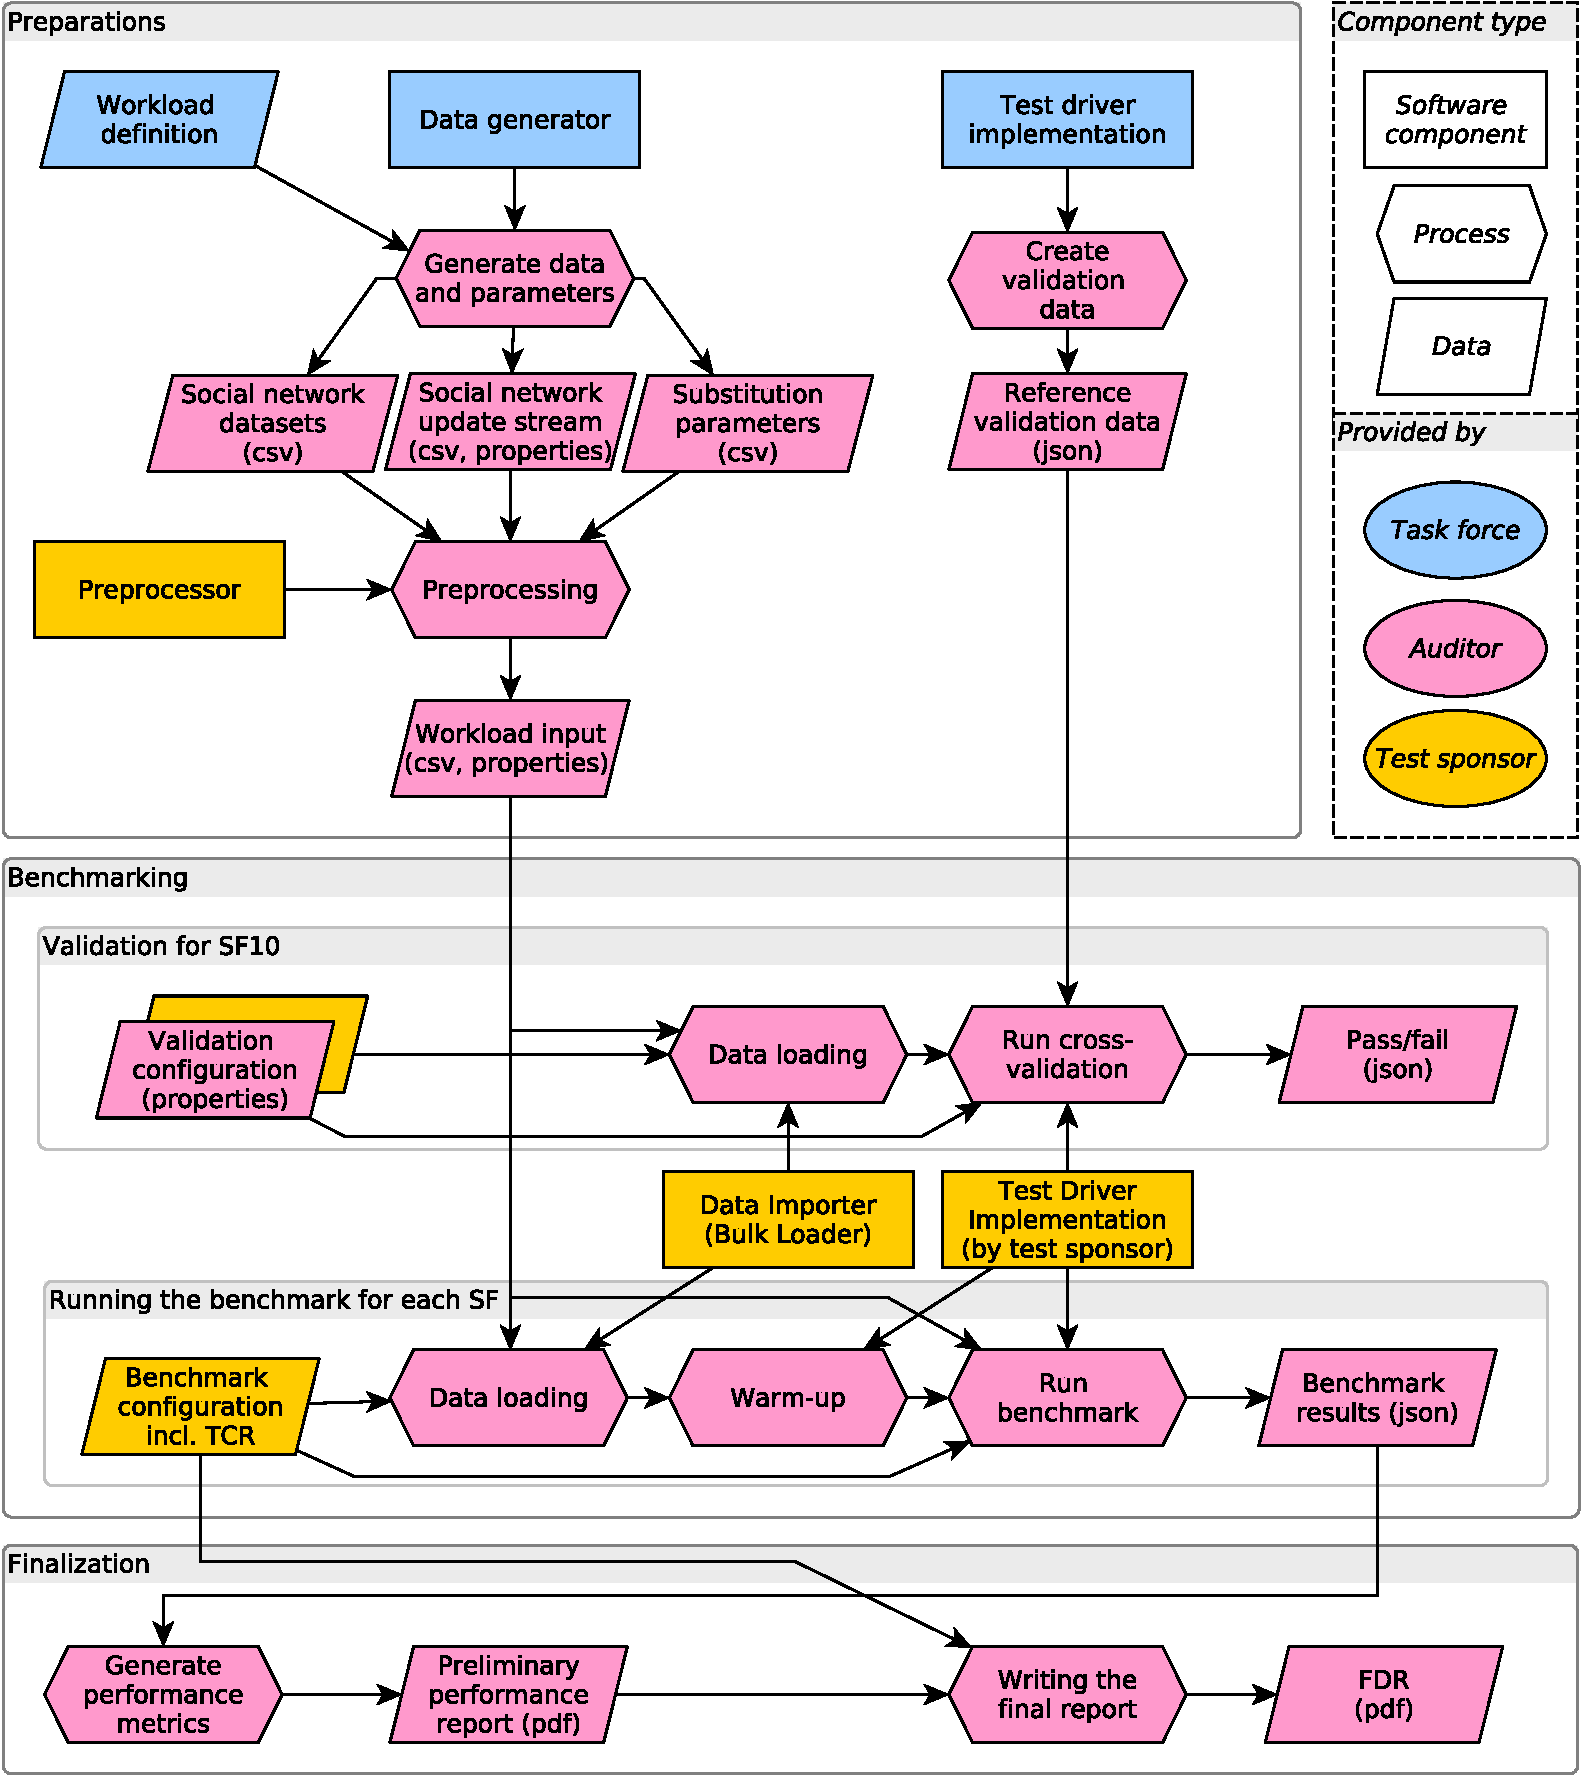
\includegraphics[scale=\yedscale]{figures/auditing-workflow}
    \caption{Benchmark execution and auditing workflow. For non-audited runs, the implementers perform the steps of the auditor.}
    \label{fig:audit-workflow}
\end{figure}

A key objective of the auditing guidelines for the Interactive workload is to \emph{allow a broad range of systems} to implement the benchmark.
Therefore, they do not impose constraints on the data model
(graph, relational, triple, \etc representations are allowed)
or on the query language
(both declarative and imperative languages are allowed).

\subsection{Scaling}
\label{sec:int-scaling}

\subsubsection{Scale Factors}

The scale factor of an SNB data set is the size of the data set in GiB of CSV (comma-separated values) files.
The size of a data set is characterized by scale factors: SF10, SF30, SF100 \etc (see \autoref{sec:scale-factors}).
All data sets contain data for three years of social network activity.

The \emph{validation run} shall be performed on the SF10 data set (see \autoref{sec:int-validation-data-set}) and use at least \numprint{100000} operations.
Note that the auditor may perform additional validation runs of the benchmark implementation using smaller data sets (\eg SF1) and issue queries.\footnote{%
An example test could be to issue complex reads with parameters such as \texttt{personId} and \texttt{messageId} selected from the \textsf{Person}/\textsf{Message} entities inserted from the update streams and cross-validate these against other systems. (The substitution parameters are taken from the initial snapshot of the graph so these nodes are not targeted by the regular workload executed by the driver.)%
}

Audited \emph{benchmark runs} of the Interactive workload shall use SF30 or larger data sets. The rationale behind this decision is to ensure that there is a sufficient number of update operations available to guarantee 2.5~hours of continuous execution (see \autoref{sec:int-measurement-window}).

% \begin{quote}
%     \emph{Rationale behind scaling.} The authors are aware that the prevalent practice for online benchmarks is to tie the reported throughput to the scale, \eg max 12.5 tpmC per warehouse in \mbox{TPC-C}. The authors depart from this practice here because with throughput tied to scale, test systems with interesting throughput rapidly become very expensive, raising the entry barrier for publishing a result. It is thought that scaling in buckets lowers the barrier of entry and reduces incentive to use hardware configurations that would be unusual in a production environment.
% \end{quote}
%COMMENTS FROM PAST GABOR TO FUTURE GABOR
%what it wants to say is that unlike TPC-C, you can get a large throughput (lots of ops) even on a small data set
%which is correct but we can ran out of updates due to the 2.5-hr simulation requirement
%so its (implied) conclusion does not hold fully hold for SNB interactive

\subsubsection{Social Network data sets}
\label{sec:int-data-sets}

\paragraph{Initial data set}
The data set is divided into a bulk loadable initial database population (90\%) and an update stream (10\%). These are generated by the SNB data generator. The data generator has options for splitting the data set into any number of files.

\paragraph{Dependencies between messages in the update stream}
The update stream contains the latest 10\% of the events in the simulated social network. These events form a single serializable sequence in time. Some events will depend on preceding events, for example a message must exist before a reply comment to the message is created. The data generator guarantees that these are separated by at least 10 seconds of simulation time.

\paragraph{Parallel updates}
The update stream may be broken into arbitrarily many sub-streams. The partition scheme is created by the \datagen. During benchmark execution, the driver preserves dependencies between update operations, such as ensuring not to refer to non-existent entities in updates (\eg a like is not added to a message which has not been inserted yet).

\subsection{Data Model and Data Loading}

\subsubsection{Supported Data Models}

SNB may be implemented with different data models (\eg relational, RDF, and different graph data models). The reference schema is provided in the specification using a UML-like notation. 


\subsubsection{Generated Input Data}
\label{sec:generated-data}

\paragraph{Storage}
The data generator produces comma-separated values (CSV) for all data models.

\paragraph{Data format}
A single attribute has a single data type, as follows:
\begin{description}
    \item [Identifier] This is an integer value foreign key or a URI in RDF. If this is an integer column, the implementation data type should support at least $2^{50}$ distinct values.
    \item [Date] A date should support a date range from 0000 to 9999 in the year field.
    \item [DateTime] A datetime should support a date range from 0000 to 9999 in the year field, with at least millisecond precision.
    \item [Short string] The string column for names may have a variable length and may have a declared maximum length, \eg 40 characters.
    \item [Long string] For example a message content may be a long string that is often short in the data but may not declare a maximum length and must support data sizes of up to 1~MB.
\end{description}

The above is stated in further detail in the benchmark specification, and it shall take precedence over the
above in the case of conflict.

A single attribute in the reference schema may not be divided into multiple attributes in the target schema.

\paragraph{Database schema}
A schema on the DBMS is optional. An RDF implementation for example may work without one. An RDF implementation is allowed to load the RDF reference schema and to take advantage of the data type and cardinality statements therein. 

\paragraph{Configuration parameters}
\datagen configuration parameters, including SF, distributions, number of persons, serialiser (\eg CsvSingularMergedFK) should be reported.

\paragraph{Primary data structures}
An RDF, relational, or graph schema may specify system specific options affecting DBMS storage layout. These may for example specify vertical partitioning. Vertical partitioning means anything from a column store layout with per-column allocated storage space to use of explicit column groups. Any mix of row or column-wise storage structures is allowed as long as this is declaratively specified on a per data structure-basis.

\paragraph{Auxiliary data structures}
Covering indices and clustered indices are allowed. If these are defined, then all replications of data implied by these must be maintained statement by statement, \ie each auxiliary data structure must be consistent with any other data structures of the table after each data manipulation operation.

A covering index is an index which materialises a specific order of a specific subset or possibly all columns of a table. 
A clustered index is an index which materialises all columns of a table in a specific order, which order may or may not be that of the primary key of the table. A clustered or covering index may be the primary or only representation of a table.

Any subset of the columns on a covering or clustered index may be used for ordering the data. A hash based index or a combination of a hash based and tree based index are all allowed, in row or column-wise or hybrid forms.

\paragraph{Loading the data}

We expect the SUT to provide some means to bulk load the data set either in the form of a dedicated offline loader component or an online loader that allows bulk inserting into a database.
The total of the bulk load time and the time for subsequent operations (indexing, computing statistics, \etc) must be reported in the FDR (see \autoref{sec:int-benchmark-workflow}).
As loading can be an expensive operation, it is allowed to conduct the audit such that the loading is only performend once, and the validation/benchmarking phases use the resulting database instance.
In practice, this can look like as follows:
(1)~load the data,
(2)~compute statistics, uniqueness constraints, keys, indices, \etc,
(3)~shut down the SUT,
(4)~create a backup of the database (\eg by copying the directory of the database).
For all subsequent runs, the database shall be restored from the backup.

\subsection{Precomputation}

Precomputation of query results (both interim and end results) is allowed. However, systems must ensure that precomputed results (\eg materialized views) are kept consistent upon updates.

\subsection{Benchmark Software Components}
\label{sec:snb-software-components}
LDBC provides a test driver, data generator, and summary reporting scripts. Benchmark implementations shall use a stable version (\eg 0.3.6) of the test driver. The SUT's database software should be a stable version that is available publicly or can be purchased at the time of the release of the audit.

\subsubsection{Adaptation of the Test Driver to a DBMS}
\label{sec:test-driver}
A qualifying run must use a test driver that adapts the provided test driver to interface with the SUT. Such an implementation, if needed, must be provided by the test sponsor. The parameter generation, result recording, and workload scheduling parts of the test driver should not be changed. The auditor must be given access to the test driver source code used in the reported run.

The test driver produces the following artefacts for each execution as a by product of the run: Start and end timestamps in wall clock time, recorded with microsecond precision. The identifier of the operation and any substitution parameters.


\subsubsection{Summary of Benchmark Results}
\label{sec:performance-metrics}
A separate test summary tool provided with the test driver analyses the test driver log(s) after a measurement window is completed. 

The tool produces for each of the distinct queries and transactions the following summary:
\begin{itemize}
    \item Run time of query in wall clock time.
    \item Count of executions.
    \item Minimum/mean/percentiles/maximum execution time.
    \item Standard deviation from the average execution time.
\end{itemize}
The tool produces for the complete run the following summary:
\begin{itemize}
    \item Operations per second for a given SF (throughput). This is the primary metric of this workload.
    \item The total execution time in wall clock time.
    \item The total number of completed operations.
\end{itemize}


\subsection{Implementation Language and Data Access Transparency}

The queries and updates may be implemented in a domain-specific query language or as procedural code written in a general-purpose programming language (\eg using the API of the database).

\subsubsection{Implementations Using a Domain-Specific Query Language}
\label{sec:snb-domain-specific-query-language}

If a domain-specific query language is used, \eg SPARQL, SQL, Cypher, or Gremlin, then explicit query plans are prohibited in all the read-only queries.%
\footnote{If the queries are not clearly declarative, the auditor must ensure that they do not specify explicit query plans by investigating their source code and experimenting with the query planner of the system (\eg using SQL's \texttt{EXPLAIN} command).}
The update transactions may still consist of multiple statements, effectively amounting to explicit plans.

Explicit query plans include but are not limited to:
\begin{itemize}
    \item Directives or hints specifying a join order or join type
    \item Directives or hints specifying an access path, \eg which index to use
    \item Directives or hints specifying an expected cardinality, selectivity, fanout or any other information that pertains to the expected number or results or cost of all or part of the query.
\end{itemize}

\begin{quote}
    \emph{Rationale behind the applied restrictions.} The updates are effectively OLTP and, therefore, the customary freedoms apply, including the use of stored procedures, however subject to access transparency. Declarative queries in a benchmark implementation should be such that they could plausibly be written by an application developer. Therefore, their formulation should not contain system specific aspects that an application developer would be unlikely to know. In other words, making a benchmark implementation should not require uncommon sophistication on behalf of the developer. This is regular practice in analytical benchmarks, \eg \mbox{TPC-H}.
\end{quote}

\subsubsection{Implementations Using a General-Purpose Programming Language}
\label{sec:snb-general-purpose-programming-language}

Implementations using a general-purpose programming language for specifying the queries (including procedural, imperative, and API-based implementations) are expected to respect the rules described in \autoref{sec:query-languages}.
For these implementations, the rules in \autoref{sec:snb-domain-specific-query-language} do not apply.

\subsection{Correctness of Benchmark Implementation}

\subsubsection{Validation data set}
\label{sec:int-validation-data-set}
The scale factor 10 shall be used as validation data set.

\subsubsection{ACID Compliance}
\label{sec:int-acid-compliance}

The Interactive workload requires full ACID support (\autoref{sec:acid-compliance}) from the SUT.
This is tested using the LDBC ACID test suite.
For the specification of this test suite, see \autoref{sec:acid-test-suite} and the related software repository at \url{https://github.com/ldbc/ldbc_acid}.

\paragraph{Expected level of isolation}
If a transaction reads the database with intent to update, the DBMS must guarantee that repeating the same read within the same transaction will return the same data. This also means that no more and no less data rows must be returned. In other words, this corresponds to snapshot or to serializable isolation. If the database is accessed without transaction context or without intent to update, then the DBMS should provide read committed semantics, \eg repeating the same read may produce different results but these results may never include effects of pending uncommitted transactions.

\paragraph{Durability and checkpoints}

A checkpoint is defined as the operation which causes data persisted in a transaction log to become durable outside of the transaction log. Specifically, this means that an SUT restart after instantaneous failure following the completion of the checkpoint may not have recourse to transaction log entries written before the end of the checkpoint.

A checkpoint typically involves a synchronisation barrier at which all data committed prior too the moment is required to be in durable storage that does not depend on the transaction log.
Not all DBMSs use a checkpointing mechanism for durability. For example a system may rely on redundant storage of data for durability guarantees against instantaneous failure of a single server.

The measurement window may contain a checkpoint. If the measurement window does not contain one, then the restart test will involve redoing all the updates in the window as part of the recovery test.

The timed window ends with an instantaneous failure of the SUT. Instantaneously killing all the SUT process(es) is adequate for simulating instantaneous failure. All these processes should be killed within one second of each other with an operating system action equivalent to the Unix \verb+kill -9+. If such is not available, then powering down each separate SUT component that has an independent power supply is also possible.

The restart test consists of restarting the SUT process(es) and finishes when the SUT is back online with all its functionality and the last successful update logged by the driver can be seen to be in effect in the database.
%In the case of a distributed (scale-out) system, a particular partition may be recovered whereas another one is still in the process of recovering. If this is so, then checking for the last update shall not be done until all partitions are online.

If the SUT hardware was powered down, the recovery period does not include the reboot and possible file system check time. The recovery time starts when the DBMS software is restarted.




\paragraph{Recovery} 
The SUT is to be restarted after the measurement window and the auditor will verify that the SUT contains the entirety of the last update recorded by the test driver(s) as successfully committed. The driver or the implementation have to make this information available. The auditor may also check the \emph{audit log} of the SUT (if available) to confirm that the operations issued by the driver were saved.

Once an official run has been validated, the recovery capabilities of the system must be tested. The system and the driver must be configured in the same way as in during the benchmark execution. After a warm-up period, an execution of the benchmark will be performed under the same terms as in the previous measured run.

\paragraph{Measuring recovery time}
At an arbitrary point close to 2 hours of wall clock time during the run, the machine will be shut down. Then, the auditor will restart the database system and will check that the last committed update (in the driver log file) is actually in the database. The auditor will measure the time taken by the system to recover from the failure. Also, all the information about how durability is ensured must be disclosed. If checkpoints are used, these must be performed with a period of 10 minutes at most.


\subsection{Benchmarking Workflow}
\label{sec:int-benchmark-workflow}

A benchmark execution is divided into the following processes (these processes are also shown in \autoref{fig:audit-workflow}):

\begin{description}
    \item[Generate data] This includes running the data generator, placing the generated files in a staging area, configuring storage, setting up the SUT configuration and preparing any data partitions in the SUT. This may include preallocating database space but may not include loading any data or defining any schema having to do with the benchmark. The \verb|ldbc.snb.interactive.update_interleave| driver parameter must come from the \verb|updateStream.properties| file, which is created by the data generator. That parameter should never be set manually. This parameter signifies the average distance of update operations in the workload.
    \item[Preprocessing] If needed, the output from the data generator is to preprocess the data set (\autoref{sec:auditing-data-format}).
    \item[Create validation data] Using one of the reference implementations of the benchmark, the reference validation data is obtained in .json format.
    \item[Data loading] The test sponsor must provide all the necessary documentation and scripts to load the data set into the database to test.
    This includes defining the database schema, if any, loading the initial database population, making this durably stored and gathering any optimiser statistics.
    The system under test must support the different data types needed by the benchmark for each of the attributes at their specified precision. No data can be filtered out, everything must be loaded. The test sponsor must provide a tool to perform arbitrary checks of the data or a shell to issue queries in a declarative language if the system supports it.
    \item[Run cross-validation] This step uses the data loader to populate the database, but the load is not timed. The validation data set is used to verify the correctness of the SUT. The auditor must load the provided data set and run the driver in validation mode, which will test that the queries provide the official results.  The benchmarking workflow will not go beyond this point unless results match the expected output.
    \item[Warm-up] Benchmark runs are preceded by a warm-up which must be performed using the LDBC driver.
    \item[Run benchmark] The bulk load time is reported and is equal to the amount of elapsed wall clock time between starting the schema definition and receiving the confirmation message of the end of statistics gathering. The workflow runs begin after the bulk load is completed. If the run does not directly follow the bulk load, it must start at a point in the update stream that has not previously been played into the database. In other words, a run may only include update events whose timestamp is later than the latest message creation date in the database prior to start of run. The run starts when the first of the test drivers send its first message to the SUT. If the SUT is running in the same process as the driver, the window starts
    when the driver starts. Also, make sure that the \verb|-rl/--results_log| is enabled. Make sure that all operations are enabled and the frequencies are those for the selected scale factor (see the exact specification of the frequencies in \autoref{sec:sf-statistics}).
\end{description}

\subsubsection{Query Timing During Benchmark Run}
\label{sec:ontime-requirements}
A valid benchmark run must last at least 2 hours of wall clock time and at most 2 hours and 15 minutes.
In order to be valid, a benchmark run needs to meet the ``95\% on-time requirement''.
The \texttt{results\_log.csv} file contains the $\mathsf{actual\_start\_time}$ and the $\mathsf{scheduled\_start\_time}$ of each of the issued queries. In order to have a valid run, 95\% of the queries must meet the following condition:
\begin{equation*}
\mathsf{actual\_start\_time} - \mathsf{scheduled\_start\_time} < 1\
\mathrm{second}
\end{equation*}

If the execution of the benchmark is valid, the auditor must retrieve all the files from directory specified by \verb|--results_dir| which includes configuration settings used, results log and results summary. All of which must be disclosed.

\subsubsection{Measurement Window}
\label{sec:int-measurement-window}

Benchmark runs execute the workload on the SUT in two phases (\autoref{fig:measurement-window-selection}).
First, the SUT must undergo a warm-up period that takes at least 30 minutes and at most 35 minutes. The goal of this is to put the system in a steady state which reflects how it would behave in a normal operating environment. The performance of the operations during warm-up is not considered.
Next, the SUT is benchmarked during a two-hour measurement window. Operation times are recorded and checked to ensure the ``95\% on-time requirement'' is satisfied.

\begin{figure}[h]
    \centering
    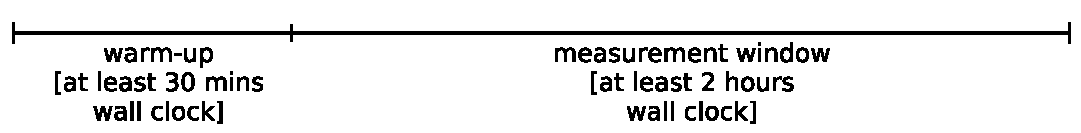
\includegraphics[width=.7\linewidth]{figures/measurement-window-selection}
    \caption{Warm-up and measurement window for benchmark run.}
    \label{fig:measurement-window-selection}
\end{figure}

The SNB \datagen produces 3~years worth data of which 10\% is used for updates (\autoref{sec:int-data-sets}), \ie approximately $3 \times 365 \times 0.1 = 109.5~\text{days} = 2628~\text{hours}$.
To ensure that the 2.5~hour wall clock period has enough input data, the lower bound of TCR is defined as 0.001 (if $2628$ hours of updates are played back at more than $1000\times$ speed, the benchmark framework runs out of updates to execute). System that can achieve a better compression (\ie lower TCR value) on a given scale factor should use larger SFs for their benchmark runs -- otherwise their total runs will be less than 2.5~hours, making them unsuitable for auditing.

%The test summary tool may be used for reading the logs created by a test driver.

\subsection{Full Disclosure Report}
\label{sec:int-fdr}

Upon successful completion of the audit, an FDR is compiled. In addition to the general requirements, the full disclosure shall cover the following:

\begin{itemize}
    \item General terms: an executive summary and declaration of the credibility of the audit
    \item System description and pricing summary: see \autoref{sec:system-config}
    \item Data generation and data loading: see \autoref{sec:generated-data}
    \item Test driver details: see \autoref{sec:test-driver}
    \item Performance metrics: see \autoref{sec:performance-metrics}
    \item Validation results: see \autoref{sec:int-validation-data-set}
    \item ACID compliance: see \autoref{sec:acid-compliance}
    \item List of supplementary materials
\end{itemize}

To ensure reproducibility of the audited results, a supplementary package is attached to the full disclosure report. This package should contain:

\begin{itemize}
    \item A README file with instructions specifying how to set up the system and run the benchmark
    \item Configuration files of the database, including database-level configuration such as buffer size and schema descriptors (if necessary)
    \item Source code or binary of a generic driver that can be used to interact with the DBMS
    \item SUT-specific LDBC driver implementation (similarly to the projects in \url{https://github.com/ldbc/ldbc_snb_interactive_v1_impls}, \url{https://github.com/ldbc/ldbc_snb_interactive_v2_impls}, \url{https://github.com/ldbc/ldbc_snb_bi})
    \item Script or instructions to compile the LDBC Java driver implementation
    \item Instructions on how to the reach the server through CLI and/or web UI (if applicable), \eg the URL (including port number), user name and password
    \item LDBC configuration files (\texttt{.properties}), including the \texttt{time\_compression\_ratio} values used in the audited runs
    \item Scripts to preprocess the input files (if necessary) and to load the data sets into the database
    \item Scripts to create validation data sets and to run the benchmark
    \item The implementations of the queries and the update operations, including their complete source code (\eg declarative queries specifications, stored procedures, \etc)
    \item Implementation of the ACID test suite
    \item Binary package of the DBMS (\eg \texttt{.deb} or \texttt{.rpm})
\end{itemize}



%%%%%%%%%%%%%%%%%%%%%%%%%%%%%%%%%%%%%%%%%%%%%%%%%%%%%%%%%%%%%%%%%%%%%%%%%%%%%%
%%%%%%%%%%%%%%%%%%%%%%%%%%%%%%%%%%%%%%%%%%%%%%%%%%%%%%%%%%%%%%%%%%%%%%%%%%%%%%
%%%%%%%%%%%%%%%%%%%%%%%%%%%%%%%%%%%%%%%%%%%%%%%%%%%%%%%%%%%%%%%%%%%%%%%%%%%%%%

\section{Auditing Rules for the Business Intelligence Workload}
\label{sec:auditing-bi-workload-audit}

%%%%%%%%%%%%%%%%%%%%%%%%%%%%%%%%%%%%%%%%%%%%%%%%%%%%%%%%%%%%%%%%%%%%%%%%%%%%%%
%%%%%%%%%%%%%%%%%%%%%%%%%%%%%%%%%%%%%%%%%%%%%%%%%%%%%%%%%%%%%%%%%%%%%%%%%%%%%%
%%%%%%%%%%%%%%%%%%%%%%%%%%%%%%%%%%%%%%%%%%%%%%%%%%%%%%%%%%%%%%%%%%%%%%%%%%%%%%

The following section describes the auditing rules specific to the Business Intelligence (BI) workload.

\subsection{Overview}
\label{sec:auditing-bi-audit-overview}

Implementing the BI workload requires the following key capabilities:

\begin{itemize}
    \item Loading the initial snapshot of the social network graph
    \item Evaluating the BI read queries (\autoref{sec:bi-reads})
    \item Evaluating the BI write operations: inserts (\autoref{sec:bi-insert-operations}) and deletes (\autoref{sec:bi-delete-operations})
    \item Performing concurrent reads and writes (\autoref{sec:auditing-bi-audit-workflow}) (optional, only allowed if ACID compliance is guaranteed)
\end{itemize}

\subsection{Workflow}
\label{sec:auditing-bi-audit-workflow}

\begin{figure}[htbp]
    \centering
    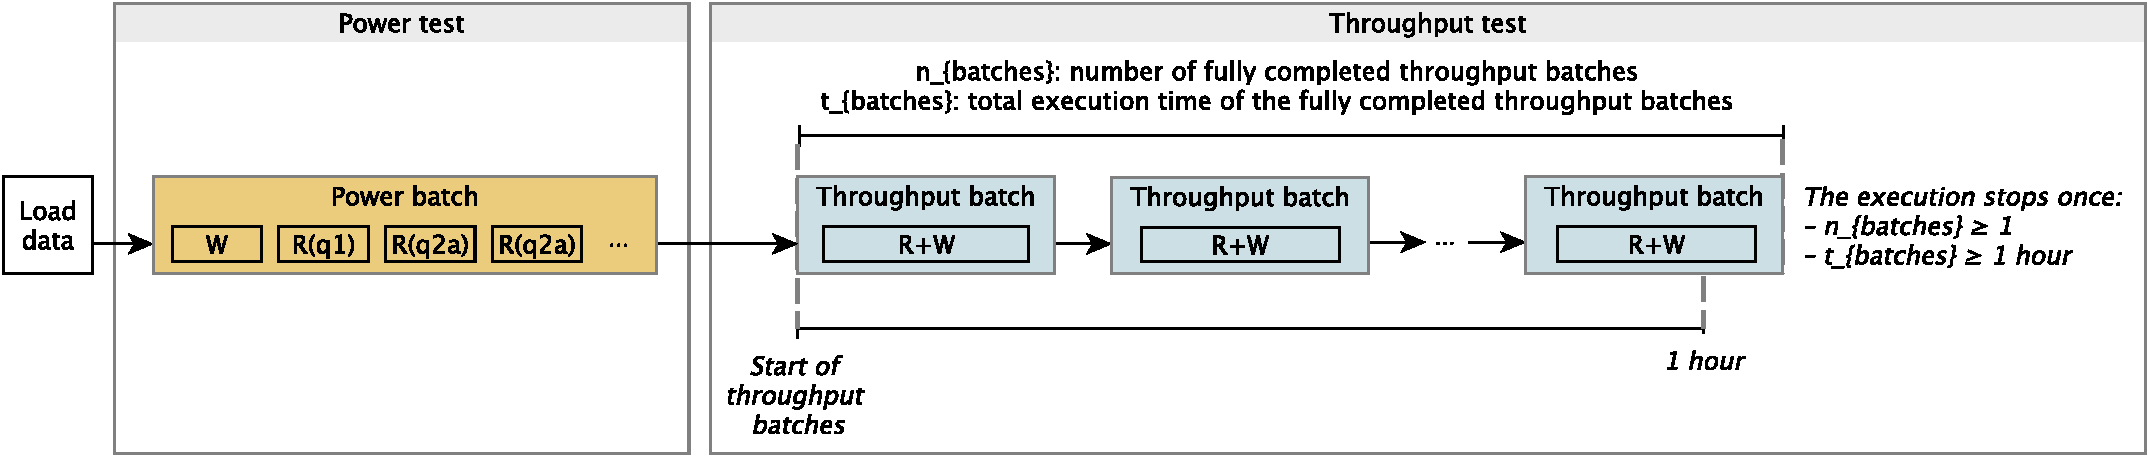
\includegraphics[scale=\yedscale]{figures/bi-batches.pdf}
    \caption{Tests and batches (power and throughput) executed in the BI workload's workflow.}
    \label{fig:bi-batches}
\end{figure}

The write operations and read queries are run in \emph{daily batches}.
In each batch, each query variant
(Q1, Q2\variantA, Q2\variantB, Q3, \ldots, Q20\variantA, Q20\variantB)
is executed using 30~different substitution parameters.
The BI workflow (\autoref{fig:bi-batches}) consists of two key parts:
the \emph{power test} (\autoref{sec:power-test}) and
the \emph{throughput test} (\autoref{sec:throughput-test}).

\subsubsection{Power Test}
\label{sec:power-test}

The \emph{power test} runs a single \emph{power batch}. This test first runs the write operations, followed by a sequential execution of individual read query variants.
The writes perform a day of inserts and deletes in the simulated social network,
while a total of $28 \times 30 = 840$ read queries are executed.

\subsubsection{Throughput Test}
\label{sec:throughput-test}

The \emph{throughput test} consists of multiple \emph{throughput batches}.
Each throughput batch runs the same type and the same amount of operations as the power batch.
However, they allow concurrent execution of the write operations and read queries in a given batch.

The execution of the throughput test during audits is the \emph{throughput measurement window}.
This window must span at least for 1~hour and
it must include at least one fully completed batch (see \autoref{fig:bi-batches}).

The workload defines two execution modes for the \emph{throughput batches}:

\begin{description}
    \item[Disjoint RW mode]
    In \emph{disjoint RW (read-write) mode} the system performs the reads and writes separately. It first executes the writes, then evaluates the read queries. Concurrency between the read operations is allowed.\\
    This mode is aimed at \emph{read-optimized data analytical systems} which do not support concurrent reads and writes. Implementations may also opt to use this mode for simplicity. For these implementations, passing the \emph{LDBC ACID compliance test} (\autoref{sec:acid-test-suite}) is not required.

    \item[Concurrent RW mode]
    In \emph{concurrent RW (read-write) mode} the system is allowed to run reads and writes concurrently. This requires the systems to be capable of handling \emph{transactions}. Implementations using this mode are required to pass the \emph{LDBC ACID compliance test} (\autoref{sec:acid-test-suite}).
\end{description}

\subsection{Runtimes}

The runtimes should be reported as follows:

\begin{itemize}
    \item The \emph{load time} ($t_\textit{load}$) denotes the time to load the data into the SUT and initialize auxiliary data structures (if applicable). For audited runs, we require that $t_\textit{load} < 24\textrm{ hours}$.
    \item The \emph{power test time} ($t_\textit{power test}$) denotes the time to perform the power test.
    \item The \emph{throughput measurement window time} ($t_\textit{throughput\ measurement}$) denotes the time to perform the throughput test, including the last (potentially unfinished) batch.
    \item The \emph{full throughput batches time} ($t_\textit{full\ throughput\ batches}$) denotes the time to evaluate the fully completed batches during the throughput measurement window.
\end{itemize}

Note that a warm-up period is not allowed (unlike the Interactive workload where such a period is required, see \autoref{sec:int-measurement-window}).

\subsection{Scoring Metrics}
\label{sec:auditing-bi-scoring-metrics}

SNBI BI provides four scoring metrics:
the \emph{power score}, the \emph{throughput score}, and their price-adjusted variants,
the \emph{per-\$ power score} and the \emph{per-\$ throughput score}.
All scores include the scale factor, denoted with ``@SF''.

\subsubsection{Price}
\label{sec:price-metrics}

We follow TPC's specification for reporting prices~\cite{tpc-pricing}.
The price is established as the \emph{total cost of ownership ($\textit{TCO}$)} for the SUT used in the benchmark,
reported as a breakdown of
machine cost,
software license costs,
and maintenance costs for 3 years.
In case of cloud deployments, the cost of running a 3-year reserved instance should be reported.
When establishing the price, the ``upfront payment'' option available at certain cloud providers should not be considered.

\subsubsection{Power Scores}
\label{sec:power-score}

The definition of \snbbi's power score follows \tpcH in using a geometric mean, ensuring that there is an incentive to improve all queries, no matter their running time.
Formally, the power score is based on the time to perform the writes
and
the time spent for executing each variant with 30~different substitution parameters, measured in seconds:
$$
\textit{power@SF} =
    \frac{\numprint{3600}}{\sqrt[29]{
        w
        \cdot q_{1}
        \cdot q_{2\variant{a}}
        \cdot q_{2\variant{b}}
        \cdot \ldots
        \cdot q_{18}
        \cdot q_{19\variant{a}}
        \cdot q_{19\variant{b}}
        \cdot q_{20\variant{a}}
        \cdot q_{20\variant{b}}
    }}
    \cdot
    \textit{SF}
$$

% Including all entries, the formula is:
% {\scriptsize
% $$
% \textit{power@SF} =
%     \frac{\numprint{3600}}{\sqrt[29]{
%         w
%         \! \cdot \! q_{1}
%         \! \cdot \! q_{2\variant{a}}
%         \! \cdot \! q_{2\variant{b}}
%         \! \cdot \! q_{2\variant{a}}
%         \! \cdot \! q_{2\variant{b}}
%         \! \cdot \! q_{3}
%         \! \cdot \! q_{4}
%         \! \cdot \! q_{5}
%         \! \cdot \! q_{6}
%         \! \cdot \! q_{7}
%         \! \cdot \! q_{8\variant{a}}
%         \! \cdot \! q_{8\variant{b}}
%         \! \cdot \! q_{9}
%         \! \cdot \! q_{10\variant{a}}
%         \! \cdot \! q_{10\variant{b}}
%         \! \cdot \! q_{11}
%         \! \cdot \! q_{12}
%         \! \cdot \! q_{13}
%         \! \cdot \! q_{14\variant{a}}
%         \! \cdot \! q_{14\variant{b}}
%         \! \cdot \! q_{15\variant{a}}
%         \! \cdot \! q_{15\variant{b}}
%         \! \cdot \! q_{16\variant{a}}
%         \! \cdot \! q_{16\variant{b}}
%         \! \cdot \! q_{17}
%         \! \cdot \! q_{18}
%         \! \cdot \! q_{19\variant{a}}
%         \! \cdot \! q_{19\variant{b}}
%         \! \cdot \! q_{20\variant{a}}
%         \! \cdot \! q_{20\variant{b}}
%     }}
%     \cdot
%     \textit{SF}
% $$
% }

To determine the price-adjusted power score, we factor in the $\textit{TCO}$\emph{:}
$$ \textit{power@SF/\$} = \textit{power@SF} \cdot \frac{\numprint{1000}}{\textit{TCO}} $$

\subsubsection{Throughput Scores}
\label{sec:throughput-score}

The throughput score is based on $t_\textit{load}$, measured in hours,
and the cumulative execution time and number of the throughput batches executed:
%throughput score is calculated as the number of batches the system could execute in a single day
$$
\textit{throughput@SF} =
    (24\text{ hours} - t_\textit{load})
    \cdot
    \frac{n_\textit{batches}}{t_\textit{batches}}
    \cdot
    \textit{SF}
$$

The subtraction of $t_\textit{load}$ ensures that the scoring rewards systems with efficient bulk loaders (unlike in \tpcH and \tpcDS which do not include load performance in their metrics).
The price-adjusted throughput score is determined analogously: % to the price-adjusted power score.
$$ \textit{throughput@SF/\$} = \textit{throughput@SF} \cdot \frac{\numprint{1000}}{\textit{TCO}} $$

\subsection{Implementation Rules}
\label{sec:auditing-bi-implementation-rules}

\subsubsection{Correctness}
\label{sec:auditing-bi-correcntess}

The SUT shall evaluate all operators correctly.
The auditor shall ascertain correctness on the SF10 data set. However, they are allowed to also use data sets of different scale factors, as well as issue custom operations (both reads and writes) to test for the correctness of the implemenation.

The validation of correctness is performed on the output of the \emph{power test} step.
The rationale for using this only step is that during concurrent execution of R/W operations in the \emph{throughput test}, it is not possible to guarantee deterministic query results, making validation impossible. Moreover, this step already includes a write batch, therefore the query results indirectly test the correctness of the implementation of write operations.

\subsubsection{Auxiliary Data Structures}
\label{sec:auditing-bi-auxiliary-data-structures}

Using auxiliary data structures (\eg indices, materialized views) is allowed if they are kept in an up-to-date state after each write operation. The full disclosure report should enumerate the auxiliary data structures used by the SUT. 

\subsubsection{Query Declarativity}
\label{sec:auditing-bi-query-declarativity}

Systems should use a domain-specific query language (\eg Cypher, Gremlin, GSQL) for the implementation, including the read queries and the update operations.
General-purpose programming languages (\eg C, C\texttt{++}, Java, Julia) are not allowed.

Implementations shall not use \emph{query-specific stored procedures written in a general-purpose programming language} (\eg a given procedure which implements BI Q5).
Using the stored procedure libraries considered to be the ``standard libraries'' of the SUT is allowed.%
\footnote{These libraries often include features such as weighted shortest path algorithms.}
Implementations may use \emph{stored procedures written in a domain-specific language}.
In cases when the categorization of the approach used by the SUT's query implementations is uncertain, it is the auditor's responsibility to decide whether the SUT complies with this rule.

\subsubsection{Query Variants}
\label{sec:auditing-bi-query-variants}

Several queries (\eg \queryRefCard{bi-read-14}{BI}{14}) use \variantA and \variantB variants with different sets of input parameters.
The SUT should not receive any hints on which variant it is currently evaluating (\eg Q14\variantA or Q14\variantB).
Moreover, it is not allowed for the query implementations to contain code that aims to detect the query variant used.

\subsection{Scaling}
\label{sec:auditing-bi-scaling}

Audited \emph{benchmark runs} of the BI workload shall use SF30 or larger data sets.
The rationale behind this decision is to ensure that there should be a sufficient number of write operations available to guarantee the execution during the duration of the measurement window (see \autoref{fig:bi-batches}).

\subsection{Full Disclosure Report}
\label{sec:auditing-bi-fdr}

The \emph{full disclosure report} (FDR) and the \emph{supplementary package} shall contain
the same information as for SNB Interactive (\autoref{sec:int-fdr}),
including, if applicable (\autoref{sec:auditing-bi-implementation-rules}), the ACID compliance report (\autoref{sec:acid-compliance}).


\bibliographystyle{abbrv}
\bibliography{references,ldbc}

\appendix

\chapter{Scale Factor Statistics}
\section{Scale Factor Statistics}\label{appendix:scale_factors}
\subsection{Scale Factor 1}

\begin{table}[H]
\centering
    \begin{tabular}{|c|c|c|c|}
    \hline
    Query Type & freq & Query Type & freq \\ 
    \hline
    \hline
    Query 1 & 26 & Query 8 & 45 \\ 
    \hline       
    Query 2 & 37 & Query 9 & 157 \\  
    \hline        
    Query 3 & 69 & Query 10 & 30 \\ 
    \hline        
    Query 4 & 36 & Query 11 & 16 \\ 
    \hline        
    Query 5 & 57 & Query 12 & 44 \\ 
    \hline        
    Query 6 & 129 & Query 13 & 19 \\  
    \hline        
    Query 7 & 87 & Query 14 & 49 \\ 
    \hline
    \end{tabular}
    \caption{Frequenceis for each query type for SF1.}
    \label{table:freqs_sf1}
\end{table}

\begin{table}[H]
    \centering
    \begin{tabular} {| l | c | c |}
        \hline
        \textbf{Entity} & \textbf{Num Entities} & \textbf{Bytes} \\
        \hline
        \hline
        comment & 2343952 & 254723836 \\
        \hline
        forum & 110202 & 6548409 \\
        \hline
        organisation & 7996 & 813270 \\
        \hline
        person & 11000 & 990357 \\
        \hline
        place & 1466 & 83667 \\
        \hline
        post & 1214766 & 138430549 \\
        \hline
        tag & 16080 & 1122429 \\
        \hline
        tagclass & 71 & 3946 \\
        \hline
        \hline
        \textbf{Relation} & \textbf{Num Relations} & \textbf{Bytes} \\
        \hline
        \hline
        comment\_hasCreator\_person & 2343952 & 63507355 \\
        \hline
        comment\_hasTag\_tag & 3069162 & 57501504 \\
        \hline
        comment\_isLocatedIn\_place & 2343952 & 39543099 \\
        \hline
        comment\_replyOf\_comment & 1187815 & 31674987 \\
        \hline
        comment\_replyOf\_post & 1156137 & 30828349 \\
        \hline
        forum\_containerOf\_post & 1214766 & 32211087 \\
        \hline
        forum\_hasMember\_person & 3260578 & 159205747 \\
        \hline
        forum\_hasModerator\_person & 110202 & 3017841 \\
        \hline
        forum\_hasTag\_tag & 355354 & 6527532 \\
        \hline
        organisation\_isLocatedIn\_place & 7996 & 79310 \\
        \hline
        person\_isLocatedIn\_place & 11000 & 196342 \\
        \hline
        person\_hasInterest\_tag & 256152 & 5120644 \\
        \hline
        person\_knows\_person & 452622 & 22659548 \\
        \hline
        person\_likes\_comment & 1649394 & 80566053 \\
        \hline
        person\_likes\_post & 1170372 & 57185940 \\
        \hline
        person\_studyAt\_organisation & 8820 & 221093 \\
        \hline
        person\_workAt\_organisation & 23969 & 581247 \\
        \hline
        place\_isPartOf\_place & 1460 & 11965 \\
        \hline
        post\_hasCreator\_person & 1214766 & 33212920 \\
        \hline
        post\_hasTag\_tag & 789735 & 14621607 \\
        \hline
        post\_isLocatedIn\_place & 1214766 & 20529353 \\
        \hline
        tag\_hasType\_tagclass & 16080 & 163348 \\
        \hline
        tagclass\_isSubclassOf\_tagclass & 70 & 616 \\
        \hline
        \hline
        \textbf{Property Files} & \textbf{Num Properties} & \textbf{Bytes} \\
        \hline
        \hline
        person\_email\_emailaddress & 18602 & 831575 \\
        \hline
        person\_speaks\_language & 24204 & 437214 \\
        \hline
        \hline
        \textbf{Total Entities} & \textbf{Total Relations} & \textbf{Total Bytes} \\
        \hline
        \hline
        3705533 & 21859120 & 1063152739 \\
        \hline
    \end{tabular}
    \caption{General statistics for SF 1}
\end{table}


\begin{table}[H]
        \centering
        \begin{tabular}{|c||r|r|r|r|}
            \hline    \multicolumn{5}{|c|}{SF = 1 }  \\
            \hline   \textbf{Clustering Coef.} &   \multicolumn{4}{|c|}{0.0484} \\
            \hline & \textbf{Min} & \textbf{Max} & \textbf{Mean} & \textbf{Median}   \\
            \hline  \textbf{\#comments/user}  &1 &  6002 & 224 & 82 \\
            \hline  \textbf{\#posts/user}  &1 &  912 & 123 & 66 \\
            \hline  \textbf{\#friends/user}  &1 &  540 & 41 & 22 \\
            \hline  \textbf{\#likes/user}  &1 &  2725 & 260 & 171 \\
            \hline
        \end{tabular}
        \caption{Detail statistics for SF 1}
\end{table}

\begin{figure}[H]
\begin{center}
  \subfigure[{\small Cumulative number of friends.}]{\label{numFriendsCumm}\includegraphics[width=0.32\textwidth,clip]{figures/scalefactor/numFriendsCumm1}}%
  \subfigure[{\small Histogram \#posts per user.}]{\label{numPostPerUsers}\includegraphics[width=0.32\textwidth,clip]{figures/scalefactor/numPostsUserHist1}}%\\[1ex]
  \subfigure[{\small Histogram \#comments per user.}]{\label{numComPerUsers}\includegraphics[width=0.32\textwidth,clip]{figures/scalefactor/numCommentsUserHist1}}
  \caption{Data distributions for SF 1}
  \label{fig:datadistSF1}
\end{center}
\end{figure}


\subsection{Scale Factor 3}

\begin{table}[H]
\centering
    \begin{tabular}{|c|c|c|c|}
    \hline
    Query Type & freq & Query Type & freq \\ 
    \hline
    \hline
    Query 1 & 26 & Query 8 & 27 \\ 
    \hline       
    Query 2 & 37 & Query 9 & 209 \\  
    \hline        
    Query 3 & 79 & Query 10 & 32 \\ 
    \hline       
    Query 4 & 36 & Query 11 & 17 \\ 
    \hline        
    Query 5 & 61 & Query 12 & 44 \\ 
    \hline        
    Query 6 & 172 & Query 13 & 19 \\  
    \hline        
    Query 7 & 72 & Query 14 & 49 \\ 
    \hline
    \end{tabular}
    \caption{Frequenceis for each query type for SF3.}
    \label{table:freqs_sf3}
\end{table}

\begin{table}[H]
    \centering
    \begin{tabular} {| l | c | c |}
        \hline
        \textbf{Entity} & \textbf{Num Entities} & \textbf{Bytes} \\
        \hline
        \hline
        comment & 7135636 & 776534811 \\
        \hline
        forum & 272268 & 16231309 \\
        \hline
        organisation & 7996 & 813270 \\
        \hline
        person & 27000 & 2431528 \\
        \hline
        place & 1466 & 83667 \\
        \hline
        post & 3140119 & 374416646 \\
        \hline
        tag & 16080 & 1122429 \\
        \hline
        tagclass & 71 & 3946 \\
        \hline
        \hline
        \textbf{Relation} & \textbf{Num Relations} & \textbf{Bytes} \\
        \hline
        \hline
        comment\_hasCreator\_person & 7135636 & 194770123 \\
        \hline
        comment\_hasTag\_tag & 9264389 & 174656230 \\
        \hline
        comment\_isLocatedIn\_place & 7135636 & 121173303 \\
        \hline
        comment\_replyOf\_comment & 3619711 & 97338366 \\
        \hline
        comment\_replyOf\_post & 3515925 & 94545033 \\
        \hline
        forum\_containerOf\_post & 3140119 & 83915474 \\
        \hline
        forum\_hasMember\_person & 9939453 & 486936117 \\
        \hline
        forum\_hasModerator\_person & 272268 & 7495375 \\
        \hline
        forum\_hasTag\_tag & 873831 & 16205018 \\
        \hline
        organisation\_isLocatedIn\_place & 7996 & 79310 \\
        \hline
        person\_isLocatedIn\_place & 27000 & 482925 \\
        \hline
        person\_hasInterest\_tag & 628563 & 12575921 \\
        \hline
        person\_knows\_person & 1370174 & 68746822 \\
        \hline
        person\_likes\_comment & 5555074 & 272259351 \\
        \hline
        person\_likes\_post & 3629288 & 177882573 \\
        \hline
        person\_studyAt\_organisation & 21574 & 541636 \\
        \hline
        person\_workAt\_organisation & 58843 & 1428856 \\
        \hline
        place\_isPartOf\_place & 1460 & 11965 \\
        \hline
        post\_hasCreator\_person & 3140119 & 86258384 \\
        \hline
        post\_hasTag\_tag & 2384629 & 44446829 \\
        \hline
        post\_isLocatedIn\_place & 3140119 & 53352987 \\
        \hline
        tag\_hasType\_tagclass & 16080 & 163348 \\
        \hline
        tagclass\_isSubclassOf\_tagclass & 70 & 616 \\
        \hline
        \hline
        \textbf{Property Files} & \textbf{Num Properties} & \textbf{Bytes} \\
        \hline
        \hline
        person\_email\_emailaddress & 45573 & 2041123 \\
        \hline
        person\_speaks\_language & 59467 & 1076428 \\
        \hline
        \hline
        \textbf{Total Entities} & \textbf{Total Relations} & \textbf{Total Bytes} \\
        \hline
        \hline
         10600636 & 64877957 & 3170021719 \\
        \hline
    \end{tabular}
    \caption{General statistics for SF 3}
\end{table}

\begin{table}[H]
    \centering
\begin{tabular}{|c||r|r|r|r|}
\hline    \multicolumn{5}{|c|}{SF = 3 }  \\
\hline   \textbf{Clustering Coef.} &   \multicolumn{4}{|c|}{0.0456} \\
\hline & \textbf{Min} & \textbf{Max} & \textbf{Mean} & \textbf{Median}   \\
\hline  \textbf{\#comments/user}  &1 &  6631 & 275 & 102 \\
\hline  \textbf{\#posts/user}  &1 &  1096 & 128 & 72 \\
\hline  \textbf{\#friends/user}  &1 &  569 & 51 & 28 \\
\hline  \textbf{\#likes/user}  &1 &  3057 & 344 & 231 \\
\hline
\end{tabular}
\caption{Detail statistics for SF 3}
\end{table}

\begin{figure}[H]
\begin{center}
  \subfigure[{\small Cumulative number of friends.}]{\label{numFriendsCumm}\includegraphics[width=0.32\textwidth,clip]{figures/scalefactor/numFriendsCumm3}}%
  \subfigure[{\small Histogram \#posts per user.}]{\label{numPostPerUsers}\includegraphics[width=0.32\textwidth,clip]{figures/scalefactor/numPostsUserHist3}}%\\[1ex]
  \subfigure[{\small Histogram \#comments per user.}]{\label{numComPerUsers}\includegraphics[width=0.32\textwidth,clip]{figures/scalefactor/numCommentsUserHist3}}
  \caption{Data distributions for SF 3}
  \label{fig:datadistSF3}
\end{center}
\end{figure}

\subsection{Scale Factor 10}

\begin{table}[H]
\centering
    \begin{tabular}{|c|c|c|c|}
    \hline
    Query Type & freq & Query Type & freq \\ 
    \hline
    \hline
    Query 1 & 26 & Query 8 & 15 \\ 
    \hline       
    Query 2 & 37 & Query 9 & 287 \\  
    \hline        
    Query 3 & 92 & Query 10 & 35 \\ 
    \hline       
    Query 4 & 36 & Query 11 & 19 \\ 
    \hline        
    Query 5 & 66 & Query 12 & 44 \\ 
    \hline        
    Query 6 & 236 & Query 13 & 19 \\  
    \hline        
    Query 7 & 54 & Query 14 & 49 \\ 
    \hline
    \end{tabular}
    \caption{Frequenceis for each query type for SF10.}
    \label{table:freqs_sf10}
\end{table}

\begin{table}[H]
    \centering
    \begin{tabular} {| l | c | c |}
        \hline
        \textbf{Entity} & \textbf{Num Entities} & \textbf{Bytes} \\
        \hline
        \hline
        comment & 24271888 & 2648214861 \\
        \hline
        forum & 729153 & 43643724 \\
        \hline
        organisation & 7996 & 813324 \\
        \hline
        person & 73000 & 6570890 \\
        \hline
        place & 1466 & 83721 \\
        \hline
        post & 8915649 & 1126585578 \\
        \hline
        tag & 16080 & 1122468 \\
        \hline
        tagclass & 71 & 3985 \\
        \hline
        \hline
        \textbf{Relation} & \textbf{Num Relations} & \textbf{Bytes} \\
        \hline
        \hline
        comment\_hasCreator\_person & 24271888 & 669164047 \\
        \hline
        comment\_hasTag\_tag & 31753457 & 605414570 \\
        \hline
        comment\_isLocatedIn\_place & 24271888 & 418145702 \\
        \hline
        comment\_replyOf\_comment & 12306670 & 336987410 \\
        \hline
        comment\_replyOf\_post & 11965218 & 327636871 \\
        \hline
        forum\_containerOf\_post & 8915649 & 242973393 \\
        \hline
        forum\_hasMember\_person & 33883607 & 1670125108 \\
        \hline
        forum\_hasModerator\_person & 729153 & 20284418 \\
        \hline
        forum\_hasTag\_tag & 2369727 & 44544367 \\
        \hline
        organisation\_isLocatedIn\_place & 7996 & 79388 \\
        \hline
        person\_isLocatedIn\_place & 73000 & 1305804 \\
        \hline
        person\_hasInterest\_tag & 1713574 & 34283207 \\
        \hline
        person\_knows\_person & 4654416 & 233569942 \\
        \hline
        person\_likes\_comment & 21418614 & 1054924693 \\
        \hline
        person\_likes\_post & 12661782 & 623979230 \\
        \hline
        person\_studyAt\_organisation & 58429 & 1467151 \\
        \hline
        person\_workAt\_organisation & 158961 & 3860488 \\
        \hline
        place\_isPartOf\_place & 1460 & 12022 \\
        \hline
        post\_hasCreator\_person & 8915649 & 247527557 \\
        \hline
        post\_hasTag\_tag & 8216364 & 154770790 \\
        \hline
        post\_isLocatedIn\_place & 8915649 & 154055825 \\
        \hline
        tag\_hasType\_tagclass & 16080 & 163408 \\
        \hline
        tagclass\_isSubclassOf\_tagclass & 70 & 691 \\
        \hline
        \hline
        \textbf{Property Files} & \textbf{Num Properties} & \textbf{Bytes} \\
        \hline
        \hline
        person\_email\_emailaddress & 124555 & 5574325 \\
        \hline
        person\_speaks\_language & 160779 & 2910238 \\
        \hline
        \hline
        \textbf{Total Entities} & \textbf{Total Relations} & \textbf{Total Bytes} \\
        \hline
        \hline
         34015303 & 217279301 & 10680799196 \\
        \hline
    \end{tabular}
    \caption{General statistics for SF 10}
\end{table}

\begin{table}[H]
\centering
\begin{tabular}{|c||r|r|r|r|}
\hline    \multicolumn{5}{|c|}{SF = 3 }  \\
\hline   \textbf{Clustering Coef.} &   \multicolumn{4}{|c|}{0.0456} \\
\hline & \textbf{Min} & \textbf{Max} & \textbf{Mean} & \textbf{Median}   \\
\hline  \textbf{\#comments/user}  &1 &  6631 & 275 & 102 \\
\hline  \textbf{\#posts/user}  &1 &  1096 & 128 & 72 \\
\hline  \textbf{\#friends/user}  &1 &  569 & 51 & 28 \\
\hline  \textbf{\#likes/user}  &1 &  3057 & 344 & 231 \\
\hline
\end{tabular}
\caption{Detail statistics for SF 10}
\end{table}

\begin{figure}[H]
\begin{center}
  \subfigure[{\small Cumulative number of friends.}]{\label{numFriendsCumm}\includegraphics[width=0.32\textwidth,clip]{figures/scalefactor/numFriendsCumm10}}%
  \subfigure[{\small Histogram \#posts per user.}]{\label{numPostPerUsers}\includegraphics[width=0.32\textwidth,clip]{figures/scalefactor/numPostsUserHist10}}%\\[1ex]
  \subfigure[{\small Histogram \#comments per user.}]{\label{numComPerUsers}\includegraphics[width=0.32\textwidth,clip]{figures/scalefactor/numCommentsUserHist10}}
  \caption{Data distributions for SF 10}
  \label{fig:datadistSF10}
\end{center}
\end{figure}

\subsection{Scale Factor 30}

\begin{table}[H]
\centering
    \begin{tabular}{|c|c|c|c|}
    \hline
    Query Type & freq & Query Type & freq \\ 
    \hline
    \hline
    Query 1 & 26 & Query 8 & 9 \\ 
    \hline       
    Query 2 & 37 & Query 9 & 384 \\  
    \hline        
    Query 3 & 106 & Query 10 & 37 \\ 
    \hline       
    Query 4 & 36 & Query 11 & 20 \\ 
    \hline        
    Query 5 & 72 & Query 12 & 44 \\ 
    \hline        
    Query 6 & 316 & Query 13 & 19 \\  
    \hline        
    Query 7 & 48 & Query 14 & 49 \\ 
    \hline
    \end{tabular}
    \caption{Frequenceis for each query type for SF30.}
    \label{table:freqs_sf30}
\end{table}

\begin{table}[H]
    \centering
    \begin{tabular} {| l | c | c |}
        \hline
        \textbf{Entity} & \textbf{Num Entities} & \textbf{Bytes} \\
        \hline
        \hline
        comment & 73590941 & 8083989095 \\
        \hline
        forum & 1842141 & 111539981 \\
        \hline
        organisation & 7996 & 813396 \\
        \hline
        person & 184000 & 16572878 \\
        \hline
        place & 1466 & 83793 \\
        \hline
        post & 23765756 & 3155561666 \\
        \hline
        tag & 16080 & 1122520 \\
        \hline
        tagclass & 71 & 4037 \\
        \hline
        \hline
        \textbf{Relation} & \textbf{Num Relations} & \textbf{Bytes} \\
        \hline
        \hline
        comment\_hasCreator\_person & 73590941 & 2088295129 \\
        \hline
        comment\_hasTag\_tag & 96053813 & 1903298754 \\
        \hline
        comment\_isLocatedIn\_place & 73590941 & 1320854361 \\
        \hline
        comment\_replyOf\_comment & 37324357 & 1075860096 \\
        \hline
        comment\_replyOf\_post & 36266584 & 1045376200 \\
        \hline
        forum\_containerOf\_post & 23765756 & 679608557 \\
        \hline
        forum\_hasMember\_person & 103901443 & 5196088120 \\
        \hline
        forum\_hasModerator\_person & 1842141 & 52580681 \\
        \hline
        forum\_hasTag\_tag & 5976729 & 116509043 \\
        \hline
        organisation\_isLocatedIn\_place & 7996 & 79492 \\
        \hline
        person\_isLocatedIn\_place & 184000 & 3297409 \\
        \hline
        person\_hasInterest\_tag & 4318588 & 86533802 \\
        \hline
        person\_knows\_person & 14212356 & 714378938 \\
        \hline
        person\_likes\_comment & 71641419 & 3584484467 \\
        \hline
        person\_likes\_post & 39694513 & 1986127459 \\
        \hline
        person\_studyAt\_organisation & 147005 & 3695367 \\
        \hline
        person\_workAt\_organisation & 401356 & 9761198 \\
        \hline
        place\_isPartOf\_place & 1460 & 12098 \\
        \hline
        post\_hasCreator\_person & 23765756 & 677464115 \\
        \hline
        post\_hasTag\_tag & 24931521 & 488840146 \\
        \hline
        post\_isLocatedIn\_place & 23765756 & 426900332 \\
        \hline
        tag\_hasType\_tagclass & 16080 & 163488 \\
        \hline
        tagclass\_isSubclassOf\_tagclass & 70 & 791 \\
        \hline
        \hline
        \textbf{Property Files} & \textbf{Num Properties} & \textbf{Bytes} \\
        \hline
        \hline
        person\_email\_emailaddress & 312925 & 14030700 \\
        \hline
        person\_speaks\_language & 405403 & 7353001 \\
        \hline
        \hline
        \textbf{Total Entities} & \textbf{Total Relations} & \textbf{Total Bytes} \\
        \hline
        \hline
         99408451 & 655400581 & 32851281110 \\
        \hline
    \end{tabular}
    \caption{General statistics for SF 30}
\end{table}

\begin{table}[H]
    \centering
\begin{tabular}{|c||r|r|r|r|}
\hline    \multicolumn{5}{|c|}{SF = 30 }  \\
\hline   \textbf{Clustering Coef.} &   \multicolumn{4}{|c|}{0.0439} \\
                            \hline & \textbf{Min} & \textbf{Max} & \textbf{Mean} & \textbf{Median}   \\
 \hline  \textbf{\#comments/user}  &1 &  7592 & 413 & 155 \\
    \hline  \textbf{\#posts/user}  &1 &  1412 & 139 & 83 \\
  \hline  \textbf{\#friends/user}  &1 &  625 & 77 & 43 \\
    \hline  \textbf{\#likes/user}  &1 &  3828 & 610 & 420 \\
\hline
\end{tabular}
\caption{Detail statistics for SF 30}
\end{table}

\begin{figure}[H]
\begin{center}
  \subfigure[{\small Cumulative number of friends.}]{\label{numFriendsCumm}\includegraphics[width=0.32\textwidth,clip]{figures/scalefactor/numFriendsCumm30}}%
  \subfigure[{\small Histogram \#posts per user.}]{\label{numPostPerUsers}\includegraphics[width=0.32\textwidth,clip]{figures/scalefactor/numPostsUserHist30}}%\\[1ex]
  \subfigure[{\small Histogram \#comments per user.}]{\label{numComPerUsers}\includegraphics[width=0.32\textwidth,clip]{figures/scalefactor/numCommentsUserHist30}}
  \caption{Data distributions for SF 30}
  \label{fig:datadistSF30}
\end{center}
\end{figure}

\subsection{Scale Factor 100}

\begin{table}[H]
\centering
    \begin{tabular}{|c|c|c|c|}
    \hline
    Query Type & freq & Query Type & freq \\ 
    \hline
    \hline
    Query 1 & 26 & Query 8 & 5 \\ 
    \hline       
    Query 2 & 37 & Query 9 & 527 \\  
    \hline        
    Query 3 & 123 & Query 10 & 40 \\ 
    \hline       
    Query 4 & 36 & Query 11 & 22  \\ 
    \hline        
    Query 5 & 78 & Query 12 & 44  \\ 
    \hline        
    Query 6 & 434 & Query 13 & 19  \\  
    \hline        
    Query 7 & 38 & Query 14 & 49  \\ 
    \hline
    \end{tabular}
    \caption{Frequenceis for each query type for SF100.}
    \label{table:freqs_sf100}
\end{table}

\begin{table}[H]
    \centering
    \begin{tabular} {| l | c | c |}
        \hline
        \textbf{Entity} & \textbf{Num Entities} & \textbf{Bytes} \\
        \hline
        \hline
        comment & 243266898 & 26732787716 \\
        \hline
        forum & 5002291 & 303107584 \\
        \hline
        organisation & 7996 & 813396 \\
        \hline
        person & 499000 & 44950237 \\
        \hline
        place & 1466 & 83793 \\
        \hline
        post & 68871360 & 9601082178 \\
        \hline
        tag & 16080 & 1122520 \\
        \hline
        tagclass & 71 & 4037 \\
        \hline
        \hline
        \textbf{Relation} & \textbf{Num Relations} & \textbf{Bytes} \\
        \hline
        \hline
        comment\_hasCreator\_person & 243266898 & 6923334782 \\
        \hline
        comment\_hasTag\_tag & 317369562 & 6310390486 \\
        \hline
        comment\_isLocatedIn\_place & 243266898 & 4380836100 \\
        \hline
        comment\_replyOf\_comment & 123386519 & 3571363911 \\
        \hline
        comment\_replyOf\_post & 119880379 & 3469854233 \\
        \hline
        forum\_containerOf\_post & 68871360 & 1977411509 \\
        \hline
        forum\_hasMember\_person & 341232279 & 17085982726 \\
        \hline
        forum\_hasModerator\_person & 5002291 & 143155976 \\
        \hline
        forum\_hasTag\_tag & 16195463 & 317441296 \\
        \hline
        organisation\_isLocatedIn\_place & 7996 & 79492 \\
        \hline
        person\_isLocatedIn\_place & 499000 & 8948068 \\
        \hline
        person\_hasInterest\_tag & 11692172 & 234436590 \\
        \hline
        person\_knows\_person & 46598276 & 2343165388 \\
        \hline
        person\_likes\_comment & 260701994 & 13062653343 \\
        \hline
        person\_likes\_post & 135205141 & 6773886764 \\
        \hline
        person\_studyAt\_organisation & 398560 & 10023920 \\
        \hline
        person\_workAt\_organisation & 1086037 & 26420132 \\
        \hline
        place\_isPartOf\_place & 1460 & 12098 \\
        \hline
        post\_hasCreator\_person & 68871360 & 1968125668 \\
        \hline
        post\_hasTag\_tag & 82466083 & 1623280287 \\
        \hline
        post\_isLocatedIn\_place & 68871360 & 1240297918 \\
        \hline
        tag\_hasType\_tagclass & 16080 & 163488 \\
        \hline
        tagclass\_isSubclassOf\_tagclass & 70 & 791 \\
        \hline
        \hline
        \textbf{Property Files} & \textbf{Num Properties} & \textbf{Bytes} \\
        \hline
        \hline
        person\_email\_emailaddress & 850804 & 38160557 \\
        \hline
        person\_speaks\_language & 1099440 & 19951911 \\
        \hline
        \hline
        \textbf{Total Entities} & \textbf{Total Relations} & \textbf{Total Bytes} \\
        \hline
        \hline
         317665162 & 2154887238 & 108213328895 \\
        \hline
    \end{tabular}
    \caption{General statistics for SF 100}
\end{table}

\begin{table}[H]
\centering
\begin{tabular}{|c||r|r|r|r|}
\hline    \multicolumn{5}{|c|}{SF = 100 }  \\
\hline   \textbf{Clustering Coef.} &   \multicolumn{4}{|c|}{0.0422} \\
                            \hline & \textbf{Min} & \textbf{Max} & \textbf{Mean} & \textbf{Median}   \\
 \hline  \textbf{\#comments/user}  &1 &  7465 & 502 & 190 \\
    \hline  \textbf{\#posts/user}  &1 &  1509 & 148 & 90 \\
  \hline  \textbf{\#friends/user}  &1 &  619 & 93 & 53 \\
    \hline  \textbf{\#likes/user}  &1 &  4312 & 799 & 556 \\
\hline
\end{tabular}
\caption{Detail statistics for SF 100}
\end{table}

\begin{figure}[H]
\begin{center}
  \subfigure[{\small Cumulative number of friends.}]{\label{numFriendsCumm}\includegraphics[width=0.32\textwidth,clip]{figures/scalefactor/numFriendsCumm100}}%
  \subfigure[{\small Histogram \#posts per user.}]{\label{numPostPerUsers}\includegraphics[width=0.32\textwidth,clip]{figures/scalefactor/numPostsUserHist100}}%\\[1ex]
  \subfigure[{\small Histogram \#comments per user.}]{\label{numComPerUsers}\includegraphics[width=0.32\textwidth,clip]{figures/scalefactor/numCommentsUserHist100}}
  \caption{Data distributions for SF 100}
  \label{fig:datadistSF10}
\end{center}
\end{figure}

\subsection{Scale Factor 300}

\begin{table}[H]
\centering
    \begin{tabular}{|c|c|c|c|}
    \hline
    Query Type & freq & Query Type & freq \\ 
    \hline
    \hline
    Query 1 & 26 & Query 8 & 3 \\ 
    \hline       
    Query 2 & 37 & Query 9 & 705 \\  
    \hline        
    Query 3 & 142 & Query 10 & 44 \\ 
    \hline       
    Query 4 & 36 & Query 11 &  24 \\ 
    \hline        
    Query 5 & 84 & Query 12 &  44 \\ 
    \hline        
    Query 6 & 580 & Query 13 &  19 \\  
    \hline        
    Query 7 & 32 & Query 14 &  49 \\ 
    \hline
    \end{tabular}
    \caption{Frequenceis for each query type for SF300.}
    \label{table:freqs_sf300}
\end{table}

\begin{table}[H]
    \centering
    \begin{tabular} {| l | c | c |}
        \hline
        \textbf{Entity} & \textbf{Num Entities} & \textbf{Bytes} \\
        \hline
        \hline
        comment & 710752235 & 78578510866 \\
        \hline
        forum & 12561079 & 769736017 \\
        \hline
        organisation & 7996 & 813396 \\
        \hline
        person & 1254000 & 113011768 \\
        \hline
        place & 1466 & 83793 \\
        \hline
        post & 182980982 & 26615002745 \\
        \hline
        tag & 16080 & 1122520 \\
        \hline
        tagclass & 71 & 4037 \\
        \hline
        \hline
        \textbf{Relation} & \textbf{Num Relations} & \textbf{Bytes} \\
        \hline
        \hline
        comment\_hasCreator\_person & 710752235 & 20740234727 \\
        \hline
        comment\_hasTag\_tag & 926124724 & 19010889474 \\
        \hline
        comment\_isLocatedIn\_place & 710752235 & 13268389734 \\
        \hline
        comment\_replyOf\_comment & 360517003 & 10910496465 \\
        \hline
        comment\_replyOf\_post & 350235232 & 10599470746 \\
        \hline
        forum\_containerOf\_post & 182980982 & 5473898610 \\
        \hline
        forum\_hasMember\_person & 995330706 & 50531158002 \\
        \hline
        forum\_hasModerator\_person & 12561079 & 368655691 \\
        \hline
        forum\_hasTag\_tag & 40653342 & 819806778 \\
        \hline
        organisation\_isLocatedIn\_place & 7996 & 79492 \\
        \hline
        person\_isLocatedIn\_place & 1254000 & 22520270 \\
        \hline
        person\_hasInterest\_tag & 29346263 & 589162363 \\
        \hline
        person\_knows\_person & 136219368 & 6857187354 \\
        \hline
        person\_likes\_comment & 820056009 & 41645511118 \\
        \hline
        person\_likes\_post & 404808353 & 20560829944 \\
        \hline
        person\_studyAt\_organisation & 1002380 & 25237062 \\
        \hline
        person\_workAt\_organisation & 2728559 & 66447988 \\
        \hline
        place\_isPartOf\_place & 1460 & 12098 \\
        \hline
        post\_hasCreator\_person & 182980982 & 5363521573 \\
        \hline
        post\_hasTag\_tag & 241151541 & 4898991661 \\
        \hline
        post\_isLocatedIn\_place & 182980982 & 3419470093 \\
        \hline
        tag\_hasType\_tagclass & 16080 & 163488 \\
        \hline
        tagclass\_isSubclassOf\_tagclass & 70 & 791 \\
        \hline
        \hline
        \textbf{Property Files} & \textbf{Num Properties} & \textbf{Bytes} \\
        \hline
        \hline
        person\_email\_emailaddress & 2140338 & 96111129 \\
        \hline
        person\_speaks\_language & 2763075 & 50221509 \\
        \hline
        \hline
        \textbf{Total Entities} & \textbf{Total Relations} & \textbf{Total Bytes} \\
        \hline
        \hline
         907573909 & 6292461581 & 321396753302 \\
        \hline
    \end{tabular}
    \caption{ General statistics for SF 300}
\end{table}

\begin{table}[H]
    \centering
\begin{tabular}{|c||r|r|r|r|}
\hline    \multicolumn{5}{|c|}{SF = 300 }  \\
\hline   \textbf{Clustering Coef.} &   \multicolumn{4}{|c|}{0.0411} \\
                            \hline & \textbf{Min} & \textbf{Max} & \textbf{Mean} & \textbf{Median}   \\
 \hline  \textbf{\#comments/user}  &1 &  8806 & 582 & 224 \\
    \hline  \textbf{\#posts/user}  &1 &  1501 & 155 & 97 \\
  \hline  \textbf{\#friends/user}  &1 &  620 & 109 & 63 \\
    \hline  \textbf{\#likes/user}  &1 &  4686 & 983 & 689 \\
\hline
\end{tabular}
\caption{Detail statistics for SF 300}
\end{table}

\begin{figure}[H]
\begin{center}
  \subfigure[{\small Cumulative number of friends.}]{\label{numFriendsCumm}\includegraphics[width=0.32\textwidth,clip]{figures/scalefactor/numFriendsCumm300}}%
  \subfigure[{\small Histogram \#posts per user.}]{\label{numPostPerUsers}\includegraphics[width=0.32\textwidth,clip]{figures/scalefactor/numPostsUserHist300}}%\\[1ex]
  \subfigure[{\small Histogram \#comments per user.}]{\label{numComPerUsers}\includegraphics[width=0.32\textwidth,clip]{figures/scalefactor/numCommentsUserHist300}}
  \caption{Data distributions for SF 300}
  \label{fig:datadistSF300}
\end{center}
\end{figure}

\subsection{Scale Factor 1000}

\begin{table}[H]
\centering
    \begin{tabular}{|c|c|c|c|}
    \hline
    Query Type & freq & Query Type & freq \\ 
    \hline
    \hline
    Query 1 & 26 & Query 8 & 1 \\ 
    \hline       
    Query 2 & 37 & Query 9 & 967 \\  
    \hline        
    Query 3 & 165 & Query 10 & 47 \\ 
    \hline       
    Query 4 & 36 & Query 11 &  26 \\ 
    \hline        
    Query 5 & 91 & Query 12 &  44 \\ 
    \hline        
    Query 6 & 796 & Query 13 &  19 \\  
    \hline        
    Query 7 & 25 & Query 14 &  49 \\ 
    \hline
    \end{tabular}
    \caption{Frequenceis for each query type for SF1000.}
    \label{table:freqs_sf1000}
\end{table}

\begin{table}[H]
\centering
\begin{tabular} {| l | c | c |}
\hline
\textbf{Entity} & \textbf{Num Entities} & \textbf{Bytes} \\
\hline \hline
comment & 2335637135 & 258944003306 \\
\hline
forum & 36098481 & 2222966076 \\
\hline
organisation & 7996 & 813396 \\
\hline
person & 3600000 & 324485964 \\
\hline
place & 1466 & 83793 \\
\hline
post & 555306166 & 83647390485 \\
\hline
tag & 16080 & 1122520 \\
\hline
tagclass & 71 & 4037 \\
\hline \hline
\textbf{Relation} & \textbf{Num Relations} & \textbf{Bytes} \\
\hline \hline
comment\_hasCreator\_person & 2335637135 & 69009917568 \\
\hline
comment\_hasTag\_tag & 3042978961 & 63451008509 \\
\hline
comment\_isLocatedIn\_place & 2335637135 & 44333145872 \\
\hline
comment\_replyOf\_comment & 1184778982 & 36597884006 \\
\hline
comment\_replyOf\_post & 1150858153 & 35549852967 \\
\hline
forum\_containerOf\_post & 555306166 & 16985930071 \\
\hline
forum\_hasMember\_person & 3277239057 & 167465482785 \\
\hline
forum\_hasModerator\_person & 36098481 & 1071895282 \\
\hline
forum\_hasTag\_tag & 116727525 & 2398752244 \\
\hline
organisation\_isLocatedIn\_place & 7996 & 79492 \\
\hline
person\_isLocatedIn\_place & 3600000 & 64736060 \\
\hline
person\_hasInterest\_tag & 84229044 & 1692899009 \\
\hline
person\_knows\_person & 447163916 & 22530441760 \\
\hline
person\_likes\_comment & 2858070323 & 146129764930 \\
\hline
person\_likes\_post & 1361722197 & 69623238723 \\
\hline
person\_studyAt\_organisation & 2878718 & 72544726 \\
\hline
person\_workAt\_organisation & 7829672 & 190876421 \\
\hline
place\_isPartOf\_place & 1460 & 12098 \\
\hline
post\_hasCreator\_person & 555306166 & 16467663132 \\
\hline
post\_hasTag\_tag & 793254841 & 16381717061 \\
\hline
post\_isLocatedIn\_place & 555306166 & 10543790321 \\
\hline
tag\_hasType\_tagclass & 16080 & 163488 \\
\hline
tagclass\_isSubclassOf\_tagclass & 70 & 791 \\
\hline \hline
\textbf{Property Files} & \textbf{Num Properties} & \textbf{Bytes} \\
\hline \hline
person\_email\_emailaddress & 6141306 & 276081939 \\
\hline
person\_speaks\_language & 7932926 & 144358836 \\
\hline \hline
\textbf{Total Entities} & \textbf{Total Relations} & \textbf{Total Bytes} \\
\hline \hline
 2930667395 & 20704648244 & 1066123107668 \\
\hline
\end{tabular}
\caption{ General statistics for SF 1000}
\end{table}

\begin{table}[H]
    \centering
    \begin{tabular}{|c||r|r|r|r|}
\hline    \multicolumn{5}{|c|}{SF = 1000 }  \\
\hline & Min & Max & Mean & Median   \\
\hline  \#posts/user  &1 &  1576 & 163 & 103 \\
\hline  \#friends/user  &1 &  636 & 124 & 73 \\
\hline
\end{tabular}
\caption{Detail statistics for SF 1000}
\end{table}

\begin{figure}[H]
\begin{center}
  \subfigure[{\small Cumulative number of friends.}]{\label{numFriendsCumm}\includegraphics[width=0.32\textwidth,clip]{figures/scalefactor/numFriendsCumm1000}}%
  \subfigure[{\small Histogram \#posts per user.}]{\label{numPostPerUsers}\includegraphics[width=0.32\textwidth,clip]{figures/scalefactor/numPostsUserHist1000}}%\\[1ex]
  \caption{Data distributions for SF 1000}
  \label{fig:datadistSF1000}
\end{center}
\end{figure}


\end{document}
